\documentclass[twoside]{book}

% Packages required by doxygen
\usepackage{fixltx2e}
\usepackage{calc}
\usepackage{doxygen}
\usepackage[export]{adjustbox} % also loads graphicx
\usepackage{graphicx}
\usepackage[utf8]{inputenc}
\usepackage{makeidx}
\usepackage{multicol}
\usepackage{multirow}
\PassOptionsToPackage{warn}{textcomp}
\usepackage{textcomp}
\usepackage[nointegrals]{wasysym}
\usepackage[table]{xcolor}

% Font selection
\usepackage[T1]{fontenc}
\usepackage[scaled=.90]{helvet}
\usepackage{courier}
\usepackage{amssymb}
\usepackage{sectsty}
\renewcommand{\familydefault}{\sfdefault}
\allsectionsfont{%
  \fontseries{bc}\selectfont%
  \color{darkgray}%
}
\renewcommand{\DoxyLabelFont}{%
  \fontseries{bc}\selectfont%
  \color{darkgray}%
}
\newcommand{\+}{\discretionary{\mbox{\scriptsize$\hookleftarrow$}}{}{}}

% Page & text layout
\usepackage{geometry}
\geometry{%
  a4paper,%
  top=2.5cm,%
  bottom=2.5cm,%
  left=2.5cm,%
  right=2.5cm%
}
\tolerance=750
\hfuzz=15pt
\hbadness=750
\setlength{\emergencystretch}{15pt}
\setlength{\parindent}{0cm}
\setlength{\parskip}{3ex plus 2ex minus 2ex}
\makeatletter
\renewcommand{\paragraph}{%
  \@startsection{paragraph}{4}{0ex}{-1.0ex}{1.0ex}{%
    \normalfont\normalsize\bfseries\SS@parafont%
  }%
}
\renewcommand{\subparagraph}{%
  \@startsection{subparagraph}{5}{0ex}{-1.0ex}{1.0ex}{%
    \normalfont\normalsize\bfseries\SS@subparafont%
  }%
}
\makeatother

% Headers & footers
\usepackage{fancyhdr}
\pagestyle{fancyplain}
\fancyhead[LE]{\fancyplain{}{\bfseries\thepage}}
\fancyhead[CE]{\fancyplain{}{}}
\fancyhead[RE]{\fancyplain{}{\bfseries\leftmark}}
\fancyhead[LO]{\fancyplain{}{\bfseries\rightmark}}
\fancyhead[CO]{\fancyplain{}{}}
\fancyhead[RO]{\fancyplain{}{\bfseries\thepage}}
\fancyfoot[LE]{\fancyplain{}{}}
\fancyfoot[CE]{\fancyplain{}{}}
\fancyfoot[RE]{\fancyplain{}{\bfseries\scriptsize Generated by Doxygen }}
\fancyfoot[LO]{\fancyplain{}{\bfseries\scriptsize Generated by Doxygen }}
\fancyfoot[CO]{\fancyplain{}{}}
\fancyfoot[RO]{\fancyplain{}{}}
\renewcommand{\footrulewidth}{0.4pt}
\renewcommand{\chaptermark}[1]{%
  \markboth{#1}{}%
}
\renewcommand{\sectionmark}[1]{%
  \markright{\thesection\ #1}%
}

% Indices & bibliography
\usepackage{natbib}
\usepackage[titles]{tocloft}
\setcounter{tocdepth}{3}
\setcounter{secnumdepth}{5}
\makeindex

% Hyperlinks (required, but should be loaded last)
\usepackage{ifpdf}
\ifpdf
  \usepackage[pdftex,pagebackref=true]{hyperref}
\else
  \usepackage[ps2pdf,pagebackref=true]{hyperref}
\fi
\hypersetup{%
  colorlinks=true,%
  linkcolor=blue,%
  citecolor=blue,%
  unicode%
}

% Custom commands
\newcommand{\clearemptydoublepage}{%
  \newpage{\pagestyle{empty}\cleardoublepage}%
}

\usepackage{caption}
\captionsetup{labelsep=space,justification=centering,font={bf},singlelinecheck=off,skip=4pt,position=top}

%===== C O N T E N T S =====

\begin{document}

% Titlepage & ToC
\hypersetup{pageanchor=false,
             bookmarksnumbered=true,
             pdfencoding=unicode
            }
\pagenumbering{alph}
\begin{titlepage}
\vspace*{7cm}
\begin{center}%
{\Large Battleship \\[1ex]\large 1.\+0.\+0 }\\
\vspace*{1cm}
{\large Generated by Doxygen 1.8.13}\\
\end{center}
\end{titlepage}
\clearemptydoublepage
\pagenumbering{roman}
\tableofcontents
\clearemptydoublepage
\pagenumbering{arabic}
\hypersetup{pageanchor=true}

%--- Begin generated contents ---
\chapter{Namespace Index}
\section{Namespace List}
Here is a list of all namespaces with brief descriptions\+:\begin{DoxyCompactList}
\item\contentsline{section}{\hyperlink{namespacebattle__ship}{battle\+\_\+ship} }{\pageref{namespacebattle__ship}}{}
\end{DoxyCompactList}

\chapter{Hierarchical Index}
\section{Class Hierarchy}
This inheritance list is sorted roughly, but not completely, alphabetically\+:\begin{DoxyCompactList}
\item \contentsline{section}{battle\+\_\+ship\+:\+:authentication}{\pageref{classbattle__ship_1_1authentication}}{}
\item \contentsline{section}{battle\+\_\+ship\+:\+:board}{\pageref{classbattle__ship_1_1board}}{}
\item \contentsline{section}{battle\+\_\+ship\+:\+:coordinates}{\pageref{structbattle__ship_1_1coordinates}}{}
\item \contentsline{section}{battle\+\_\+ship\+:\+:game}{\pageref{classbattle__ship_1_1game}}{}
\item \contentsline{section}{battle\+\_\+ship\+:\+:geometry}{\pageref{classbattle__ship_1_1geometry}}{}
\item \contentsline{section}{battle\+\_\+ship\+:\+:highscore\+\_\+manager}{\pageref{classbattle__ship_1_1highscore__manager}}{}
\item \contentsline{section}{battle\+\_\+ship\+:\+:market}{\pageref{classbattle__ship_1_1market}}{}
\item \contentsline{section}{battle\+\_\+ship\+:\+:notification\+\_\+manager}{\pageref{classbattle__ship_1_1notification__manager}}{}
\item \contentsline{section}{battle\+\_\+ship\+:\+:piece}{\pageref{classbattle__ship_1_1piece}}{}
\begin{DoxyCompactList}
\item \contentsline{section}{battle\+\_\+ship\+:\+:vessel}{\pageref{classbattle__ship_1_1vessel}}{}
\begin{DoxyCompactList}
\item \contentsline{section}{battle\+\_\+ship\+:\+:carrier}{\pageref{classbattle__ship_1_1carrier}}{}
\item \contentsline{section}{battle\+\_\+ship\+:\+:cruiser}{\pageref{classbattle__ship_1_1cruiser}}{}
\item \contentsline{section}{battle\+\_\+ship\+:\+:destroyer}{\pageref{classbattle__ship_1_1destroyer}}{}
\item \contentsline{section}{battle\+\_\+ship\+:\+:raft}{\pageref{classbattle__ship_1_1raft}}{}
\item \contentsline{section}{battle\+\_\+ship\+:\+:submarine}{\pageref{classbattle__ship_1_1submarine}}{}
\end{DoxyCompactList}
\end{DoxyCompactList}
\item \contentsline{section}{battle\+\_\+ship\+:\+:player}{\pageref{classbattle__ship_1_1player}}{}
\begin{DoxyCompactList}
\item \contentsline{section}{battle\+\_\+ship\+:\+:human}{\pageref{classbattle__ship_1_1human}}{}
\item \contentsline{section}{battle\+\_\+ship\+:\+:npc}{\pageref{classbattle__ship_1_1npc}}{}
\end{DoxyCompactList}
\item \contentsline{section}{battle\+\_\+ship\+:\+:rules}{\pageref{classbattle__ship_1_1rules}}{}
\item \contentsline{section}{battle\+\_\+ship\+:\+:screen\+\_\+manager}{\pageref{classbattle__ship_1_1screen__manager}}{}
\end{DoxyCompactList}

\chapter{Class Index}
\section{Class List}
Here are the classes, structs, unions and interfaces with brief descriptions\+:\begin{DoxyCompactList}
\item\contentsline{section}{\hyperlink{classbattle__ship_1_1authentication}{battle\+\_\+ship\+::authentication} }{\pageref{classbattle__ship_1_1authentication}}{}
\item\contentsline{section}{\hyperlink{classbattle__ship_1_1board}{battle\+\_\+ship\+::board} }{\pageref{classbattle__ship_1_1board}}{}
\item\contentsline{section}{\hyperlink{classbattle__ship_1_1carrier}{battle\+\_\+ship\+::carrier} }{\pageref{classbattle__ship_1_1carrier}}{}
\item\contentsline{section}{\hyperlink{structbattle__ship_1_1coordinates}{battle\+\_\+ship\+::coordinates} }{\pageref{structbattle__ship_1_1coordinates}}{}
\item\contentsline{section}{\hyperlink{classbattle__ship_1_1cruiser}{battle\+\_\+ship\+::cruiser} }{\pageref{classbattle__ship_1_1cruiser}}{}
\item\contentsline{section}{\hyperlink{classbattle__ship_1_1destroyer}{battle\+\_\+ship\+::destroyer} }{\pageref{classbattle__ship_1_1destroyer}}{}
\item\contentsline{section}{\hyperlink{classbattle__ship_1_1game}{battle\+\_\+ship\+::game} }{\pageref{classbattle__ship_1_1game}}{}
\item\contentsline{section}{\hyperlink{classbattle__ship_1_1geometry}{battle\+\_\+ship\+::geometry} }{\pageref{classbattle__ship_1_1geometry}}{}
\item\contentsline{section}{\hyperlink{classbattle__ship_1_1highscore__manager}{battle\+\_\+ship\+::highscore\+\_\+manager} }{\pageref{classbattle__ship_1_1highscore__manager}}{}
\item\contentsline{section}{\hyperlink{classbattle__ship_1_1human}{battle\+\_\+ship\+::human} }{\pageref{classbattle__ship_1_1human}}{}
\item\contentsline{section}{\hyperlink{classbattle__ship_1_1market}{battle\+\_\+ship\+::market} }{\pageref{classbattle__ship_1_1market}}{}
\item\contentsline{section}{\hyperlink{classbattle__ship_1_1notification__manager}{battle\+\_\+ship\+::notification\+\_\+manager} }{\pageref{classbattle__ship_1_1notification__manager}}{}
\item\contentsline{section}{\hyperlink{classbattle__ship_1_1npc}{battle\+\_\+ship\+::npc} }{\pageref{classbattle__ship_1_1npc}}{}
\item\contentsline{section}{\hyperlink{classbattle__ship_1_1piece}{battle\+\_\+ship\+::piece} }{\pageref{classbattle__ship_1_1piece}}{}
\item\contentsline{section}{\hyperlink{classbattle__ship_1_1player}{battle\+\_\+ship\+::player} }{\pageref{classbattle__ship_1_1player}}{}
\item\contentsline{section}{\hyperlink{classbattle__ship_1_1raft}{battle\+\_\+ship\+::raft} }{\pageref{classbattle__ship_1_1raft}}{}
\item\contentsline{section}{\hyperlink{classbattle__ship_1_1rules}{battle\+\_\+ship\+::rules} }{\pageref{classbattle__ship_1_1rules}}{}
\item\contentsline{section}{\hyperlink{classbattle__ship_1_1screen__manager}{battle\+\_\+ship\+::screen\+\_\+manager} }{\pageref{classbattle__ship_1_1screen__manager}}{}
\item\contentsline{section}{\hyperlink{classbattle__ship_1_1submarine}{battle\+\_\+ship\+::submarine} }{\pageref{classbattle__ship_1_1submarine}}{}
\item\contentsline{section}{\hyperlink{classbattle__ship_1_1vessel}{battle\+\_\+ship\+::vessel} }{\pageref{classbattle__ship_1_1vessel}}{}
\end{DoxyCompactList}

\chapter{File Index}
\section{File List}
Here is a list of all files with brief descriptions\+:\begin{DoxyCompactList}
\item\contentsline{section}{include/\hyperlink{authentication_8h}{authentication.\+h} }{\pageref{authentication_8h}}{}
\item\contentsline{section}{include/\hyperlink{board_8h}{board.\+h} }{\pageref{board_8h}}{}
\item\contentsline{section}{include/\hyperlink{carrier_8h}{carrier.\+h} }{\pageref{carrier_8h}}{}
\item\contentsline{section}{include/\hyperlink{coordinates_8h}{coordinates.\+h} }{\pageref{coordinates_8h}}{}
\item\contentsline{section}{include/\hyperlink{cruiser_8h}{cruiser.\+h} }{\pageref{cruiser_8h}}{}
\item\contentsline{section}{include/\hyperlink{destroyer_8h}{destroyer.\+h} }{\pageref{destroyer_8h}}{}
\item\contentsline{section}{include/\hyperlink{game_8h}{game.\+h} }{\pageref{game_8h}}{}
\item\contentsline{section}{include/\hyperlink{geometry_8h}{geometry.\+h} }{\pageref{geometry_8h}}{}
\item\contentsline{section}{include/\hyperlink{highscore__manager_8h}{highscore\+\_\+manager.\+h} }{\pageref{highscore__manager_8h}}{}
\item\contentsline{section}{include/\hyperlink{human_8h}{human.\+h} }{\pageref{human_8h}}{}
\item\contentsline{section}{include/\hyperlink{market_8h}{market.\+h} }{\pageref{market_8h}}{}
\item\contentsline{section}{include/\hyperlink{notification__manager_8h}{notification\+\_\+manager.\+h} }{\pageref{notification__manager_8h}}{}
\item\contentsline{section}{include/\hyperlink{npc_8h}{npc.\+h} }{\pageref{npc_8h}}{}
\item\contentsline{section}{include/\hyperlink{piece_8h}{piece.\+h} }{\pageref{piece_8h}}{}
\item\contentsline{section}{include/\hyperlink{player_8h}{player.\+h} }{\pageref{player_8h}}{}
\item\contentsline{section}{include/\hyperlink{raft_8h}{raft.\+h} }{\pageref{raft_8h}}{}
\item\contentsline{section}{include/\hyperlink{rules_8h}{rules.\+h} }{\pageref{rules_8h}}{}
\item\contentsline{section}{include/\hyperlink{screen__manager_8h}{screen\+\_\+manager.\+h} }{\pageref{screen__manager_8h}}{}
\item\contentsline{section}{include/\hyperlink{submarine_8h}{submarine.\+h} }{\pageref{submarine_8h}}{}
\item\contentsline{section}{include/\hyperlink{vessel_8h}{vessel.\+h} }{\pageref{vessel_8h}}{}
\item\contentsline{section}{src/\hyperlink{authentication_8cpp}{authentication.\+cpp} }{\pageref{authentication_8cpp}}{}
\item\contentsline{section}{src/\hyperlink{battle_8cpp}{battle.\+cpp} }{\pageref{battle_8cpp}}{}
\item\contentsline{section}{src/\hyperlink{board_8cpp}{board.\+cpp} }{\pageref{board_8cpp}}{}
\item\contentsline{section}{src/\hyperlink{coordinates_8cpp}{coordinates.\+cpp} }{\pageref{coordinates_8cpp}}{}
\item\contentsline{section}{src/\hyperlink{game_8cpp}{game.\+cpp} }{\pageref{game_8cpp}}{}
\item\contentsline{section}{src/\hyperlink{geometry_8cpp}{geometry.\+cpp} }{\pageref{geometry_8cpp}}{}
\item\contentsline{section}{src/\hyperlink{highscore__manager_8cpp}{highscore\+\_\+manager.\+cpp} }{\pageref{highscore__manager_8cpp}}{}
\item\contentsline{section}{src/\hyperlink{human_8cpp}{human.\+cpp} }{\pageref{human_8cpp}}{}
\item\contentsline{section}{src/\hyperlink{market_8cpp}{market.\+cpp} }{\pageref{market_8cpp}}{}
\item\contentsline{section}{src/\hyperlink{notification__manager_8cpp}{notification\+\_\+manager.\+cpp} }{\pageref{notification__manager_8cpp}}{}
\item\contentsline{section}{src/\hyperlink{npc_8cpp}{npc.\+cpp} }{\pageref{npc_8cpp}}{}
\item\contentsline{section}{src/\hyperlink{player_8cpp}{player.\+cpp} }{\pageref{player_8cpp}}{}
\item\contentsline{section}{src/\hyperlink{screen__manager_8cpp}{screen\+\_\+manager.\+cpp} }{\pageref{screen__manager_8cpp}}{}
\item\contentsline{section}{src/\hyperlink{vessel_8cpp}{vessel.\+cpp} }{\pageref{vessel_8cpp}}{}
\end{DoxyCompactList}

\chapter{Namespace Documentation}
\hypertarget{namespacebattle__ship}{}\section{battle\+\_\+ship Namespace Reference}
\label{namespacebattle__ship}\index{battle\+\_\+ship@{battle\+\_\+ship}}
\subsection*{Classes}
\begin{DoxyCompactItemize}
\item 
class \hyperlink{classbattle__ship_1_1authentication}{authentication}
\begin{DoxyCompactList}\small\item\em Class used for login and signup. \end{DoxyCompactList}\item 
class \hyperlink{classbattle__ship_1_1board}{board}
\begin{DoxyCompactList}\small\item\em Class used to handle board state. \end{DoxyCompactList}\item 
class \hyperlink{classbattle__ship_1_1carrier}{carrier}
\begin{DoxyCompactList}\small\item\em A type of vessel. \end{DoxyCompactList}\item 
struct \hyperlink{structbattle__ship_1_1coordinates}{coordinates}
\begin{DoxyCompactList}\small\item\em Used to define points on a board. \end{DoxyCompactList}\item 
class \hyperlink{classbattle__ship_1_1cruiser}{cruiser}
\begin{DoxyCompactList}\small\item\em A type of vessel. \end{DoxyCompactList}\item 
class \hyperlink{classbattle__ship_1_1destroyer}{destroyer}
\begin{DoxyCompactList}\small\item\em A type of vessel. \end{DoxyCompactList}\item 
class \hyperlink{classbattle__ship_1_1game}{game}
\begin{DoxyCompactList}\small\item\em Holds the current battle state. \end{DoxyCompactList}\item 
class \hyperlink{classbattle__ship_1_1geometry}{geometry}
\begin{DoxyCompactList}\small\item\em Used to hold geometrical algorithms. \end{DoxyCompactList}\item 
class \hyperlink{classbattle__ship_1_1highscore__manager}{highscore\+\_\+manager}
\begin{DoxyCompactList}\small\item\em Used to hold all highscores and mange the highscore state. \end{DoxyCompactList}\item 
class \hyperlink{classbattle__ship_1_1human}{human}
\begin{DoxyCompactList}\small\item\em A type of player Implements methods targeted for playable characters (human controlled) \end{DoxyCompactList}\item 
class \hyperlink{classbattle__ship_1_1market__manager}{market\+\_\+manager}
\begin{DoxyCompactList}\small\item\em Used to manage available vessels and transactions via budget checking. \end{DoxyCompactList}\item 
class \hyperlink{classbattle__ship_1_1notification__manager}{notification\+\_\+manager}
\begin{DoxyCompactList}\small\item\em Used to manage all notifications state. \end{DoxyCompactList}\item 
class \hyperlink{classbattle__ship_1_1npc}{npc}
\begin{DoxyCompactList}\small\item\em A type of player, implements methods targeted for non-\/playable characters (computer controlled) \end{DoxyCompactList}\item 
class \hyperlink{classbattle__ship_1_1piece}{piece}
\begin{DoxyCompactList}\small\item\em Abstract/\+Interface for classes of type piece. \end{DoxyCompactList}\item 
class \hyperlink{classbattle__ship_1_1player}{player}
\begin{DoxyCompactList}\small\item\em Abstract class for a player. \end{DoxyCompactList}\item 
class \hyperlink{classbattle__ship_1_1raft}{raft}
\begin{DoxyCompactList}\small\item\em A type of vessel. \end{DoxyCompactList}\item 
class \hyperlink{classbattle__ship_1_1screen__manager}{screen\+\_\+manager}
\begin{DoxyCompactList}\small\item\em Class used to output to terminal in three coloumns. \end{DoxyCompactList}\item 
class \hyperlink{classbattle__ship_1_1submarine}{submarine}
\begin{DoxyCompactList}\small\item\em A type of vessel. \end{DoxyCompactList}\item 
class \hyperlink{classbattle__ship_1_1vessel}{vessel}
\begin{DoxyCompactList}\small\item\em Implements the methods for the abstract piece class. \end{DoxyCompactList}\end{DoxyCompactItemize}
\subsection*{Enumerations}
\begin{DoxyCompactItemize}
\item 
enum \hyperlink{namespacebattle__ship_ab3bfa90e413692dac2d4463364f80561}{x\+\_\+axis} \{ \newline
\hyperlink{namespacebattle__ship_ab3bfa90e413692dac2d4463364f80561a7fc56270e7a70fa81a5935b72eacbe29}{x\+\_\+axis\+::A} = 1, 
\hyperlink{namespacebattle__ship_ab3bfa90e413692dac2d4463364f80561a9d5ed678fe57bcca610140957afab571}{x\+\_\+axis\+::B} = 2, 
\hyperlink{namespacebattle__ship_ab3bfa90e413692dac2d4463364f80561a0d61f8370cad1d412f80b84d143e1257}{x\+\_\+axis\+::C} = 3, 
\hyperlink{namespacebattle__ship_ab3bfa90e413692dac2d4463364f80561af623e75af30e62bbd73d6df5b50bb7b5}{x\+\_\+axis\+::D} = 4, 
\newline
\hyperlink{namespacebattle__ship_ab3bfa90e413692dac2d4463364f80561a3a3ea00cfc35332cedf6e5e9a32e94da}{x\+\_\+axis\+::E} = 5, 
\hyperlink{namespacebattle__ship_ab3bfa90e413692dac2d4463364f80561a800618943025315f869e4e1f09471012}{x\+\_\+axis\+::F} = 6, 
\hyperlink{namespacebattle__ship_ab3bfa90e413692dac2d4463364f80561adfcf28d0734569a6a693bc8194de62bf}{x\+\_\+axis\+::G} = 7, 
\hyperlink{namespacebattle__ship_ab3bfa90e413692dac2d4463364f80561ac1d9f50f86825a1a2302ec2449c17196}{x\+\_\+axis\+::H} = 8, 
\newline
\hyperlink{namespacebattle__ship_ab3bfa90e413692dac2d4463364f80561add7536794b63bf90eccfd37f9b147d7f}{x\+\_\+axis\+::I} = 9, 
\hyperlink{namespacebattle__ship_ab3bfa90e413692dac2d4463364f80561aff44570aca8241914870afbc310cdb85}{x\+\_\+axis\+::J} = 10
 \}
\item 
enum \hyperlink{namespacebattle__ship_aed87488f0a73f0d0679fe343fb61c784}{orientation} \{ \hyperlink{namespacebattle__ship_aed87488f0a73f0d0679fe343fb61c784a4505cad087312551a6fbbe6ebe163e0f}{orientation\+::horizontal}, 
\hyperlink{namespacebattle__ship_aed87488f0a73f0d0679fe343fb61c784ae6dec152d6a941fccb0a5e8cc2579cc3}{orientation\+::vertical}
 \}
\end{DoxyCompactItemize}
\subsection*{Functions}
\begin{DoxyCompactItemize}
\item 
std\+::ostream \& \hyperlink{namespacebattle__ship_a8f319aebd93115655c5cfd648a988e01}{operator$<$$<$} (std\+::ostream \&os, const \hyperlink{classbattle__ship_1_1board}{board} \&b)
\item 
std\+::ostream \& \hyperlink{namespacebattle__ship_ac73c2d37116f5d6ed25e71eef5c37dc8}{operator$<$$<$} (std\+::ostream \&os, const \hyperlink{structbattle__ship_1_1coordinates}{coordinates} \&p)
\item 
bool \hyperlink{namespacebattle__ship_ab0747cf7357f5f11e76979fdf9757861}{operator$>$$>$} (std\+::istream \&is, \hyperlink{structbattle__ship_1_1coordinates}{coordinates} \&p)
\item 
std\+::ostream \& \hyperlink{namespacebattle__ship_a1a93528abeff933fb4839aa528313c51}{operator$<$$<$} (std\+::ostream \&os, const \hyperlink{classbattle__ship_1_1notification__manager}{notification\+\_\+manager} \&n)
\end{DoxyCompactItemize}


\subsection{Enumeration Type Documentation}
\mbox{\Hypertarget{namespacebattle__ship_aed87488f0a73f0d0679fe343fb61c784}\label{namespacebattle__ship_aed87488f0a73f0d0679fe343fb61c784}} 
\index{battle\+\_\+ship@{battle\+\_\+ship}!orientation@{orientation}}
\index{orientation@{orientation}!battle\+\_\+ship@{battle\+\_\+ship}}
\subsubsection{\texorpdfstring{orientation}{orientation}}
{\footnotesize\ttfamily enum \hyperlink{namespacebattle__ship_aed87488f0a73f0d0679fe343fb61c784}{battle\+\_\+ship\+::orientation}\hspace{0.3cm}{\ttfamily [strong]}}

\begin{DoxyEnumFields}{Enumerator}
\raisebox{\heightof{T}}[0pt][0pt]{\index{horizontal@{horizontal}!battle\+\_\+ship@{battle\+\_\+ship}}\index{battle\+\_\+ship@{battle\+\_\+ship}!horizontal@{horizontal}}}\mbox{\Hypertarget{namespacebattle__ship_aed87488f0a73f0d0679fe343fb61c784a4505cad087312551a6fbbe6ebe163e0f}\label{namespacebattle__ship_aed87488f0a73f0d0679fe343fb61c784a4505cad087312551a6fbbe6ebe163e0f}} 
horizontal&\\
\hline

\raisebox{\heightof{T}}[0pt][0pt]{\index{vertical@{vertical}!battle\+\_\+ship@{battle\+\_\+ship}}\index{battle\+\_\+ship@{battle\+\_\+ship}!vertical@{vertical}}}\mbox{\Hypertarget{namespacebattle__ship_aed87488f0a73f0d0679fe343fb61c784ae6dec152d6a941fccb0a5e8cc2579cc3}\label{namespacebattle__ship_aed87488f0a73f0d0679fe343fb61c784ae6dec152d6a941fccb0a5e8cc2579cc3}} 
vertical&\\
\hline

\end{DoxyEnumFields}


Definition at line 19 of file coordinates.\+h.

\mbox{\Hypertarget{namespacebattle__ship_ab3bfa90e413692dac2d4463364f80561}\label{namespacebattle__ship_ab3bfa90e413692dac2d4463364f80561}} 
\index{battle\+\_\+ship@{battle\+\_\+ship}!x\+\_\+axis@{x\+\_\+axis}}
\index{x\+\_\+axis@{x\+\_\+axis}!battle\+\_\+ship@{battle\+\_\+ship}}
\subsubsection{\texorpdfstring{x\+\_\+axis}{x\_axis}}
{\footnotesize\ttfamily enum \hyperlink{namespacebattle__ship_ab3bfa90e413692dac2d4463364f80561}{battle\+\_\+ship\+::x\+\_\+axis}\hspace{0.3cm}{\ttfamily [strong]}}

\begin{DoxyEnumFields}{Enumerator}
\raisebox{\heightof{T}}[0pt][0pt]{\index{A@{A}!battle\+\_\+ship@{battle\+\_\+ship}}\index{battle\+\_\+ship@{battle\+\_\+ship}!A@{A}}}\mbox{\Hypertarget{namespacebattle__ship_ab3bfa90e413692dac2d4463364f80561a7fc56270e7a70fa81a5935b72eacbe29}\label{namespacebattle__ship_ab3bfa90e413692dac2d4463364f80561a7fc56270e7a70fa81a5935b72eacbe29}} 
A&\\
\hline

\raisebox{\heightof{T}}[0pt][0pt]{\index{B@{B}!battle\+\_\+ship@{battle\+\_\+ship}}\index{battle\+\_\+ship@{battle\+\_\+ship}!B@{B}}}\mbox{\Hypertarget{namespacebattle__ship_ab3bfa90e413692dac2d4463364f80561a9d5ed678fe57bcca610140957afab571}\label{namespacebattle__ship_ab3bfa90e413692dac2d4463364f80561a9d5ed678fe57bcca610140957afab571}} 
B&\\
\hline

\raisebox{\heightof{T}}[0pt][0pt]{\index{C@{C}!battle\+\_\+ship@{battle\+\_\+ship}}\index{battle\+\_\+ship@{battle\+\_\+ship}!C@{C}}}\mbox{\Hypertarget{namespacebattle__ship_ab3bfa90e413692dac2d4463364f80561a0d61f8370cad1d412f80b84d143e1257}\label{namespacebattle__ship_ab3bfa90e413692dac2d4463364f80561a0d61f8370cad1d412f80b84d143e1257}} 
C&\\
\hline

\raisebox{\heightof{T}}[0pt][0pt]{\index{D@{D}!battle\+\_\+ship@{battle\+\_\+ship}}\index{battle\+\_\+ship@{battle\+\_\+ship}!D@{D}}}\mbox{\Hypertarget{namespacebattle__ship_ab3bfa90e413692dac2d4463364f80561af623e75af30e62bbd73d6df5b50bb7b5}\label{namespacebattle__ship_ab3bfa90e413692dac2d4463364f80561af623e75af30e62bbd73d6df5b50bb7b5}} 
D&\\
\hline

\raisebox{\heightof{T}}[0pt][0pt]{\index{E@{E}!battle\+\_\+ship@{battle\+\_\+ship}}\index{battle\+\_\+ship@{battle\+\_\+ship}!E@{E}}}\mbox{\Hypertarget{namespacebattle__ship_ab3bfa90e413692dac2d4463364f80561a3a3ea00cfc35332cedf6e5e9a32e94da}\label{namespacebattle__ship_ab3bfa90e413692dac2d4463364f80561a3a3ea00cfc35332cedf6e5e9a32e94da}} 
E&\\
\hline

\raisebox{\heightof{T}}[0pt][0pt]{\index{F@{F}!battle\+\_\+ship@{battle\+\_\+ship}}\index{battle\+\_\+ship@{battle\+\_\+ship}!F@{F}}}\mbox{\Hypertarget{namespacebattle__ship_ab3bfa90e413692dac2d4463364f80561a800618943025315f869e4e1f09471012}\label{namespacebattle__ship_ab3bfa90e413692dac2d4463364f80561a800618943025315f869e4e1f09471012}} 
F&\\
\hline

\raisebox{\heightof{T}}[0pt][0pt]{\index{G@{G}!battle\+\_\+ship@{battle\+\_\+ship}}\index{battle\+\_\+ship@{battle\+\_\+ship}!G@{G}}}\mbox{\Hypertarget{namespacebattle__ship_ab3bfa90e413692dac2d4463364f80561adfcf28d0734569a6a693bc8194de62bf}\label{namespacebattle__ship_ab3bfa90e413692dac2d4463364f80561adfcf28d0734569a6a693bc8194de62bf}} 
G&\\
\hline

\raisebox{\heightof{T}}[0pt][0pt]{\index{H@{H}!battle\+\_\+ship@{battle\+\_\+ship}}\index{battle\+\_\+ship@{battle\+\_\+ship}!H@{H}}}\mbox{\Hypertarget{namespacebattle__ship_ab3bfa90e413692dac2d4463364f80561ac1d9f50f86825a1a2302ec2449c17196}\label{namespacebattle__ship_ab3bfa90e413692dac2d4463364f80561ac1d9f50f86825a1a2302ec2449c17196}} 
H&\\
\hline

\raisebox{\heightof{T}}[0pt][0pt]{\index{I@{I}!battle\+\_\+ship@{battle\+\_\+ship}}\index{battle\+\_\+ship@{battle\+\_\+ship}!I@{I}}}\mbox{\Hypertarget{namespacebattle__ship_ab3bfa90e413692dac2d4463364f80561add7536794b63bf90eccfd37f9b147d7f}\label{namespacebattle__ship_ab3bfa90e413692dac2d4463364f80561add7536794b63bf90eccfd37f9b147d7f}} 
I&\\
\hline

\raisebox{\heightof{T}}[0pt][0pt]{\index{J@{J}!battle\+\_\+ship@{battle\+\_\+ship}}\index{battle\+\_\+ship@{battle\+\_\+ship}!J@{J}}}\mbox{\Hypertarget{namespacebattle__ship_ab3bfa90e413692dac2d4463364f80561aff44570aca8241914870afbc310cdb85}\label{namespacebattle__ship_ab3bfa90e413692dac2d4463364f80561aff44570aca8241914870afbc310cdb85}} 
J&\\
\hline

\end{DoxyEnumFields}


Definition at line 6 of file coordinates.\+h.



\subsection{Function Documentation}
\mbox{\Hypertarget{namespacebattle__ship_ac73c2d37116f5d6ed25e71eef5c37dc8}\label{namespacebattle__ship_ac73c2d37116f5d6ed25e71eef5c37dc8}} 
\index{battle\+\_\+ship@{battle\+\_\+ship}!operator$<$$<$@{operator$<$$<$}}
\index{operator$<$$<$@{operator$<$$<$}!battle\+\_\+ship@{battle\+\_\+ship}}
\subsubsection{\texorpdfstring{operator$<$$<$()}{operator<<()}\hspace{0.1cm}{\footnotesize\ttfamily [1/3]}}
{\footnotesize\ttfamily std\+::ostream\& battle\+\_\+ship\+::operator$<$$<$ (\begin{DoxyParamCaption}\item[{std\+::ostream \&}]{os,  }\item[{const \hyperlink{structbattle__ship_1_1coordinates}{coordinates} \&}]{p }\end{DoxyParamCaption})}



Definition at line 8 of file coordinates.\+cpp.

\mbox{\Hypertarget{namespacebattle__ship_a1a93528abeff933fb4839aa528313c51}\label{namespacebattle__ship_a1a93528abeff933fb4839aa528313c51}} 
\index{battle\+\_\+ship@{battle\+\_\+ship}!operator$<$$<$@{operator$<$$<$}}
\index{operator$<$$<$@{operator$<$$<$}!battle\+\_\+ship@{battle\+\_\+ship}}
\subsubsection{\texorpdfstring{operator$<$$<$()}{operator<<()}\hspace{0.1cm}{\footnotesize\ttfamily [2/3]}}
{\footnotesize\ttfamily std\+::ostream\& battle\+\_\+ship\+::operator$<$$<$ (\begin{DoxyParamCaption}\item[{std\+::ostream \&}]{os,  }\item[{const \hyperlink{classbattle__ship_1_1notification__manager}{notification\+\_\+manager} \&}]{n }\end{DoxyParamCaption})}



Definition at line 10 of file notification\+\_\+manager.\+cpp.

\mbox{\Hypertarget{namespacebattle__ship_a8f319aebd93115655c5cfd648a988e01}\label{namespacebattle__ship_a8f319aebd93115655c5cfd648a988e01}} 
\index{battle\+\_\+ship@{battle\+\_\+ship}!operator$<$$<$@{operator$<$$<$}}
\index{operator$<$$<$@{operator$<$$<$}!battle\+\_\+ship@{battle\+\_\+ship}}
\subsubsection{\texorpdfstring{operator$<$$<$()}{operator<<()}\hspace{0.1cm}{\footnotesize\ttfamily [3/3]}}
{\footnotesize\ttfamily std\+::ostream\& battle\+\_\+ship\+::operator$<$$<$ (\begin{DoxyParamCaption}\item[{std\+::ostream \&}]{os,  }\item[{const \hyperlink{classbattle__ship_1_1board}{board} \&}]{b }\end{DoxyParamCaption})}

Mostly self explanatory, the method used A\+N\+SI escape characters to display different colours to show a coordinate which is hit, miss, empty or poulated 

Definition at line 211 of file board.\+cpp.

\mbox{\Hypertarget{namespacebattle__ship_ab0747cf7357f5f11e76979fdf9757861}\label{namespacebattle__ship_ab0747cf7357f5f11e76979fdf9757861}} 
\index{battle\+\_\+ship@{battle\+\_\+ship}!operator$>$$>$@{operator$>$$>$}}
\index{operator$>$$>$@{operator$>$$>$}!battle\+\_\+ship@{battle\+\_\+ship}}
\subsubsection{\texorpdfstring{operator$>$$>$()}{operator>>()}}
{\footnotesize\ttfamily bool battle\+\_\+ship\+::operator$>$$>$ (\begin{DoxyParamCaption}\item[{std\+::istream \&}]{is,  }\item[{\hyperlink{structbattle__ship_1_1coordinates}{coordinates} \&}]{p }\end{DoxyParamCaption})}

This method works by searching using Reg\+Ex for a specific letter and one to two digits. Validation on this for ranges is done and if all checks pass a coordinate is created. 

Definition at line 20 of file coordinates.\+cpp.


\chapter{Class Documentation}
\hypertarget{classbattle__ship_1_1authentication}{}\section{battle\+\_\+ship\+:\+:authentication Class Reference}
\label{classbattle__ship_1_1authentication}\index{battle\+\_\+ship\+::authentication@{battle\+\_\+ship\+::authentication}}


Class used for login and signup.  




{\ttfamily \#include $<$authentication.\+h$>$}

\subsection*{Static Public Member Functions}
\begin{DoxyCompactItemize}
\item 
static void \hyperlink{classbattle__ship_1_1authentication_aeb0c243e25547624235a562f657cfd63}{signup} (std\+::shared\+\_\+ptr$<$ \hyperlink{classbattle__ship_1_1human}{human} $>$ \&p)
\item 
static void \hyperlink{classbattle__ship_1_1authentication_a27046f1ace46e91bd6412ed35ddf0242}{signin} (std\+::shared\+\_\+ptr$<$ \hyperlink{classbattle__ship_1_1human}{human} $>$ \&p)
\end{DoxyCompactItemize}


\subsection{Detailed Description}
Class used for login and signup. 

\begin{DoxyAuthor}{Author}
Enrico Zammit Lonardelli
\end{DoxyAuthor}
Contact\+: \href{mailto:enrico.zammitl@gmail.com}{\tt enrico.\+zammitl@gmail.\+com}

Created on\+: Tue, 14 Apr 2020 14\+:25\+:47 

Definition at line 17 of file authentication.\+h.



\subsection{Member Function Documentation}
\mbox{\Hypertarget{classbattle__ship_1_1authentication_a27046f1ace46e91bd6412ed35ddf0242}\label{classbattle__ship_1_1authentication_a27046f1ace46e91bd6412ed35ddf0242}} 
\index{battle\+\_\+ship\+::authentication@{battle\+\_\+ship\+::authentication}!signin@{signin}}
\index{signin@{signin}!battle\+\_\+ship\+::authentication@{battle\+\_\+ship\+::authentication}}
\subsubsection{\texorpdfstring{signin()}{signin()}}
{\footnotesize\ttfamily void battle\+\_\+ship\+::authentication\+::signin (\begin{DoxyParamCaption}\item[{std\+::shared\+\_\+ptr$<$ \hyperlink{classbattle__ship_1_1human}{human} $>$ \&}]{p }\end{DoxyParamCaption})\hspace{0.3cm}{\ttfamily [static]}}



Definition at line 43 of file authentication.\+cpp.

\mbox{\Hypertarget{classbattle__ship_1_1authentication_aeb0c243e25547624235a562f657cfd63}\label{classbattle__ship_1_1authentication_aeb0c243e25547624235a562f657cfd63}} 
\index{battle\+\_\+ship\+::authentication@{battle\+\_\+ship\+::authentication}!signup@{signup}}
\index{signup@{signup}!battle\+\_\+ship\+::authentication@{battle\+\_\+ship\+::authentication}}
\subsubsection{\texorpdfstring{signup()}{signup()}}
{\footnotesize\ttfamily void battle\+\_\+ship\+::authentication\+::signup (\begin{DoxyParamCaption}\item[{std\+::shared\+\_\+ptr$<$ \hyperlink{classbattle__ship_1_1human}{human} $>$ \&}]{p }\end{DoxyParamCaption})\hspace{0.3cm}{\ttfamily [static]}}



Definition at line 11 of file authentication.\+cpp.



The documentation for this class was generated from the following files\+:\begin{DoxyCompactItemize}
\item 
include/\hyperlink{authentication_8h}{authentication.\+h}\item 
src/\hyperlink{authentication_8cpp}{authentication.\+cpp}\end{DoxyCompactItemize}

\hypertarget{classbattle__ship_1_1board}{}\section{battle\+\_\+ship\+:\+:board Class Reference}
\label{classbattle__ship_1_1board}\index{battle\+\_\+ship\+::board@{battle\+\_\+ship\+::board}}


{\ttfamily \#include $<$board.\+h$>$}

\subsection*{Public Member Functions}
\begin{DoxyCompactItemize}
\item 
\hyperlink{classbattle__ship_1_1board_a4d561505fe0c5d355e70bbd2bde1b00e}{board} ()
\item 
\hyperlink{classbattle__ship_1_1board_a72bdef4b84b4c2d8241b4307cae2cb9e}{board} (const \hyperlink{classbattle__ship_1_1board}{board} \&b)
\item 
\hyperlink{classbattle__ship_1_1board}{board} \& \hyperlink{classbattle__ship_1_1board_a4349c045147f686d09cdc47690f15e34}{operator=} (const \hyperlink{classbattle__ship_1_1board}{board} \&b)
\item 
\hyperlink{classbattle__ship_1_1board_aae7ac9e7bbd44c1b2d7a745721936ee2}{board} (\hyperlink{classbattle__ship_1_1board}{board} \&\&b)
\item 
\hyperlink{classbattle__ship_1_1board}{board} \& \hyperlink{classbattle__ship_1_1board_ae6dc011dea24157e59e2b3a6f34af586}{operator=} (\hyperlink{classbattle__ship_1_1board}{board} \&\&b)
\item 
\hyperlink{classbattle__ship_1_1board_a06d4ef9b5cb2dbb7aa4516464ff1ec52}{$\sim$board} ()=default
\item 
std\+::size\+\_\+t \hyperlink{classbattle__ship_1_1board_a74cf4399466cad172160f005da6d45fa}{get\+\_\+rows} () const
\item 
std\+::size\+\_\+t \hyperlink{classbattle__ship_1_1board_ad3d5995d4b8a0af0cfc802a1731f6a6d}{get\+\_\+cols} () const
\item 
std\+::vector$<$ std\+::unique\+\_\+ptr$<$ \hyperlink{classbattle__ship_1_1piece}{battle\+\_\+ship\+::piece} $>$ $>$ const  \& \hyperlink{classbattle__ship_1_1board_a12358d2f6eabd200d7f4e8f7276ffc96}{get\+\_\+pieces} ()
\item 
std\+::size\+\_\+t \hyperlink{classbattle__ship_1_1board_a6469025697317ca96be621908464a2c0}{index} (const \hyperlink{structbattle__ship_1_1coordinates}{battle\+\_\+ship\+::coordinates} \&p) const
\item 
std\+::size\+\_\+t \hyperlink{classbattle__ship_1_1board_aea7bba93d5c16b0c550b5874e0ce04a7}{get\+\_\+size} () const
\item 
void \hyperlink{classbattle__ship_1_1board_a9dd8f7b3681cc8ed1c5309a796f377e2}{modify\+\_\+coordinate} (\hyperlink{structbattle__ship_1_1coordinates}{battle\+\_\+ship\+::coordinates} \&target\+\_\+coordinates, std\+::string new\+\_\+value)
\item 
void \hyperlink{classbattle__ship_1_1board_a19d236125f444778e5789109d9c1093b}{remove\+\_\+piece} (size\+\_\+t pos)
\item 
void \hyperlink{classbattle__ship_1_1board_a3f6a458721d6f0cfbf167f5568539296}{edit\+\_\+piece} (\hyperlink{classbattle__ship_1_1piece}{battle\+\_\+ship\+::piece} \&p, size\+\_\+t pos, \hyperlink{structbattle__ship_1_1coordinates}{battle\+\_\+ship\+::coordinates} new\+\_\+coor, \hyperlink{namespacebattle__ship_aed87488f0a73f0d0679fe343fb61c784}{battle\+\_\+ship\+::orientation} new\+\_\+orientation)
\item 
void \hyperlink{classbattle__ship_1_1board_a9afa4baeef0df47e4a2efe05de9cb8eb}{operator$<$$<$} (std\+::unique\+\_\+ptr$<$ \hyperlink{classbattle__ship_1_1piece}{battle\+\_\+ship\+::piece} $>$ p)
\item 
std\+::string \hyperlink{classbattle__ship_1_1board_ade89ae8272e10d6c47a8d4f2c2927d0a}{operator()} (const \hyperlink{structbattle__ship_1_1coordinates}{battle\+\_\+ship\+::coordinates} \&p) const
\end{DoxyCompactItemize}
\subsection*{Friends}
\begin{DoxyCompactItemize}
\item 
std\+::ostream \& \hyperlink{classbattle__ship_1_1board_a1a31fc970cf43cac6d5b1a44e3831f5d}{operator$<$$<$} (std\+::ostream \&os, const \hyperlink{classbattle__ship_1_1board}{board} \&b)
\end{DoxyCompactItemize}


\subsection{Detailed Description}


Definition at line 14 of file board.\+h.



\subsection{Constructor \& Destructor Documentation}
\mbox{\Hypertarget{classbattle__ship_1_1board_a4d561505fe0c5d355e70bbd2bde1b00e}\label{classbattle__ship_1_1board_a4d561505fe0c5d355e70bbd2bde1b00e}} 
\index{battle\+\_\+ship\+::board@{battle\+\_\+ship\+::board}!board@{board}}
\index{board@{board}!battle\+\_\+ship\+::board@{battle\+\_\+ship\+::board}}
\subsubsection{\texorpdfstring{board()}{board()}\hspace{0.1cm}{\footnotesize\ttfamily [1/3]}}
{\footnotesize\ttfamily battle\+\_\+ship\+::board\+::board (\begin{DoxyParamCaption}{ }\end{DoxyParamCaption})}



Definition at line 12 of file board.\+cpp.

\mbox{\Hypertarget{classbattle__ship_1_1board_a72bdef4b84b4c2d8241b4307cae2cb9e}\label{classbattle__ship_1_1board_a72bdef4b84b4c2d8241b4307cae2cb9e}} 
\index{battle\+\_\+ship\+::board@{battle\+\_\+ship\+::board}!board@{board}}
\index{board@{board}!battle\+\_\+ship\+::board@{battle\+\_\+ship\+::board}}
\subsubsection{\texorpdfstring{board()}{board()}\hspace{0.1cm}{\footnotesize\ttfamily [2/3]}}
{\footnotesize\ttfamily battle\+\_\+ship\+::board\+::board (\begin{DoxyParamCaption}\item[{const \hyperlink{classbattle__ship_1_1board}{board} \&}]{b }\end{DoxyParamCaption})}



Definition at line 22 of file board.\+cpp.

\mbox{\Hypertarget{classbattle__ship_1_1board_aae7ac9e7bbd44c1b2d7a745721936ee2}\label{classbattle__ship_1_1board_aae7ac9e7bbd44c1b2d7a745721936ee2}} 
\index{battle\+\_\+ship\+::board@{battle\+\_\+ship\+::board}!board@{board}}
\index{board@{board}!battle\+\_\+ship\+::board@{battle\+\_\+ship\+::board}}
\subsubsection{\texorpdfstring{board()}{board()}\hspace{0.1cm}{\footnotesize\ttfamily [3/3]}}
{\footnotesize\ttfamily battle\+\_\+ship\+::board\+::board (\begin{DoxyParamCaption}\item[{\hyperlink{classbattle__ship_1_1board}{board} \&\&}]{b }\end{DoxyParamCaption})}



Definition at line 68 of file board.\+cpp.

\mbox{\Hypertarget{classbattle__ship_1_1board_a06d4ef9b5cb2dbb7aa4516464ff1ec52}\label{classbattle__ship_1_1board_a06d4ef9b5cb2dbb7aa4516464ff1ec52}} 
\index{battle\+\_\+ship\+::board@{battle\+\_\+ship\+::board}!````~board@{$\sim$board}}
\index{````~board@{$\sim$board}!battle\+\_\+ship\+::board@{battle\+\_\+ship\+::board}}
\subsubsection{\texorpdfstring{$\sim$board()}{~board()}}
{\footnotesize\ttfamily battle\+\_\+ship\+::board\+::$\sim$board (\begin{DoxyParamCaption}{ }\end{DoxyParamCaption})\hspace{0.3cm}{\ttfamily [default]}}



\subsection{Member Function Documentation}
\mbox{\Hypertarget{classbattle__ship_1_1board_a3f6a458721d6f0cfbf167f5568539296}\label{classbattle__ship_1_1board_a3f6a458721d6f0cfbf167f5568539296}} 
\index{battle\+\_\+ship\+::board@{battle\+\_\+ship\+::board}!edit\+\_\+piece@{edit\+\_\+piece}}
\index{edit\+\_\+piece@{edit\+\_\+piece}!battle\+\_\+ship\+::board@{battle\+\_\+ship\+::board}}
\subsubsection{\texorpdfstring{edit\+\_\+piece()}{edit\_piece()}}
{\footnotesize\ttfamily void battle\+\_\+ship\+::board\+::edit\+\_\+piece (\begin{DoxyParamCaption}\item[{\hyperlink{classbattle__ship_1_1piece}{battle\+\_\+ship\+::piece} \&}]{p,  }\item[{size\+\_\+t}]{pos,  }\item[{\hyperlink{structbattle__ship_1_1coordinates}{battle\+\_\+ship\+::coordinates}}]{new\+\_\+coor,  }\item[{\hyperlink{namespacebattle__ship_aed87488f0a73f0d0679fe343fb61c784}{battle\+\_\+ship\+::orientation}}]{new\+\_\+orientation }\end{DoxyParamCaption})}



Definition at line 157 of file board.\+cpp.

\mbox{\Hypertarget{classbattle__ship_1_1board_ad3d5995d4b8a0af0cfc802a1731f6a6d}\label{classbattle__ship_1_1board_ad3d5995d4b8a0af0cfc802a1731f6a6d}} 
\index{battle\+\_\+ship\+::board@{battle\+\_\+ship\+::board}!get\+\_\+cols@{get\+\_\+cols}}
\index{get\+\_\+cols@{get\+\_\+cols}!battle\+\_\+ship\+::board@{battle\+\_\+ship\+::board}}
\subsubsection{\texorpdfstring{get\+\_\+cols()}{get\_cols()}}
{\footnotesize\ttfamily std\+::size\+\_\+t battle\+\_\+ship\+::board\+::get\+\_\+cols (\begin{DoxyParamCaption}{ }\end{DoxyParamCaption}) const\hspace{0.3cm}{\ttfamily [inline]}}



Definition at line 32 of file board.\+h.

\mbox{\Hypertarget{classbattle__ship_1_1board_a12358d2f6eabd200d7f4e8f7276ffc96}\label{classbattle__ship_1_1board_a12358d2f6eabd200d7f4e8f7276ffc96}} 
\index{battle\+\_\+ship\+::board@{battle\+\_\+ship\+::board}!get\+\_\+pieces@{get\+\_\+pieces}}
\index{get\+\_\+pieces@{get\+\_\+pieces}!battle\+\_\+ship\+::board@{battle\+\_\+ship\+::board}}
\subsubsection{\texorpdfstring{get\+\_\+pieces()}{get\_pieces()}}
{\footnotesize\ttfamily std\+::vector$<$std\+::unique\+\_\+ptr$<$\hyperlink{classbattle__ship_1_1piece}{battle\+\_\+ship\+::piece}$>$ $>$ const\& battle\+\_\+ship\+::board\+::get\+\_\+pieces (\begin{DoxyParamCaption}{ }\end{DoxyParamCaption})\hspace{0.3cm}{\ttfamily [inline]}}



Definition at line 33 of file board.\+h.

\mbox{\Hypertarget{classbattle__ship_1_1board_a74cf4399466cad172160f005da6d45fa}\label{classbattle__ship_1_1board_a74cf4399466cad172160f005da6d45fa}} 
\index{battle\+\_\+ship\+::board@{battle\+\_\+ship\+::board}!get\+\_\+rows@{get\+\_\+rows}}
\index{get\+\_\+rows@{get\+\_\+rows}!battle\+\_\+ship\+::board@{battle\+\_\+ship\+::board}}
\subsubsection{\texorpdfstring{get\+\_\+rows()}{get\_rows()}}
{\footnotesize\ttfamily std\+::size\+\_\+t battle\+\_\+ship\+::board\+::get\+\_\+rows (\begin{DoxyParamCaption}{ }\end{DoxyParamCaption}) const\hspace{0.3cm}{\ttfamily [inline]}}



Definition at line 31 of file board.\+h.

\mbox{\Hypertarget{classbattle__ship_1_1board_aea7bba93d5c16b0c550b5874e0ce04a7}\label{classbattle__ship_1_1board_aea7bba93d5c16b0c550b5874e0ce04a7}} 
\index{battle\+\_\+ship\+::board@{battle\+\_\+ship\+::board}!get\+\_\+size@{get\+\_\+size}}
\index{get\+\_\+size@{get\+\_\+size}!battle\+\_\+ship\+::board@{battle\+\_\+ship\+::board}}
\subsubsection{\texorpdfstring{get\+\_\+size()}{get\_size()}}
{\footnotesize\ttfamily std\+::size\+\_\+t battle\+\_\+ship\+::board\+::get\+\_\+size (\begin{DoxyParamCaption}{ }\end{DoxyParamCaption}) const\hspace{0.3cm}{\ttfamily [inline]}}



Definition at line 37 of file board.\+h.

\mbox{\Hypertarget{classbattle__ship_1_1board_a6469025697317ca96be621908464a2c0}\label{classbattle__ship_1_1board_a6469025697317ca96be621908464a2c0}} 
\index{battle\+\_\+ship\+::board@{battle\+\_\+ship\+::board}!index@{index}}
\index{index@{index}!battle\+\_\+ship\+::board@{battle\+\_\+ship\+::board}}
\subsubsection{\texorpdfstring{index()}{index()}}
{\footnotesize\ttfamily std\+::size\+\_\+t battle\+\_\+ship\+::board\+::index (\begin{DoxyParamCaption}\item[{const \hyperlink{structbattle__ship_1_1coordinates}{battle\+\_\+ship\+::coordinates} \&}]{p }\end{DoxyParamCaption}) const}



Definition at line 87 of file board.\+cpp.

\mbox{\Hypertarget{classbattle__ship_1_1board_a9dd8f7b3681cc8ed1c5309a796f377e2}\label{classbattle__ship_1_1board_a9dd8f7b3681cc8ed1c5309a796f377e2}} 
\index{battle\+\_\+ship\+::board@{battle\+\_\+ship\+::board}!modify\+\_\+coordinate@{modify\+\_\+coordinate}}
\index{modify\+\_\+coordinate@{modify\+\_\+coordinate}!battle\+\_\+ship\+::board@{battle\+\_\+ship\+::board}}
\subsubsection{\texorpdfstring{modify\+\_\+coordinate()}{modify\_coordinate()}}
{\footnotesize\ttfamily void battle\+\_\+ship\+::board\+::modify\+\_\+coordinate (\begin{DoxyParamCaption}\item[{\hyperlink{structbattle__ship_1_1coordinates}{battle\+\_\+ship\+::coordinates} \&}]{target\+\_\+coordinates,  }\item[{std\+::string}]{new\+\_\+value }\end{DoxyParamCaption})}



Definition at line 152 of file board.\+cpp.

\mbox{\Hypertarget{classbattle__ship_1_1board_ade89ae8272e10d6c47a8d4f2c2927d0a}\label{classbattle__ship_1_1board_ade89ae8272e10d6c47a8d4f2c2927d0a}} 
\index{battle\+\_\+ship\+::board@{battle\+\_\+ship\+::board}!operator()@{operator()}}
\index{operator()@{operator()}!battle\+\_\+ship\+::board@{battle\+\_\+ship\+::board}}
\subsubsection{\texorpdfstring{operator()()}{operator()()}}
{\footnotesize\ttfamily std\+::string battle\+\_\+ship\+::board\+::operator() (\begin{DoxyParamCaption}\item[{const \hyperlink{structbattle__ship_1_1coordinates}{battle\+\_\+ship\+::coordinates} \&}]{p }\end{DoxyParamCaption}) const}



Definition at line 97 of file board.\+cpp.

\mbox{\Hypertarget{classbattle__ship_1_1board_a9afa4baeef0df47e4a2efe05de9cb8eb}\label{classbattle__ship_1_1board_a9afa4baeef0df47e4a2efe05de9cb8eb}} 
\index{battle\+\_\+ship\+::board@{battle\+\_\+ship\+::board}!operator$<$$<$@{operator$<$$<$}}
\index{operator$<$$<$@{operator$<$$<$}!battle\+\_\+ship\+::board@{battle\+\_\+ship\+::board}}
\subsubsection{\texorpdfstring{operator$<$$<$()}{operator<<()}}
{\footnotesize\ttfamily void battle\+\_\+ship\+::board\+::operator$<$$<$ (\begin{DoxyParamCaption}\item[{std\+::unique\+\_\+ptr$<$ \hyperlink{classbattle__ship_1_1piece}{battle\+\_\+ship\+::piece} $>$}]{p }\end{DoxyParamCaption})}



Definition at line 101 of file board.\+cpp.

\mbox{\Hypertarget{classbattle__ship_1_1board_a4349c045147f686d09cdc47690f15e34}\label{classbattle__ship_1_1board_a4349c045147f686d09cdc47690f15e34}} 
\index{battle\+\_\+ship\+::board@{battle\+\_\+ship\+::board}!operator=@{operator=}}
\index{operator=@{operator=}!battle\+\_\+ship\+::board@{battle\+\_\+ship\+::board}}
\subsubsection{\texorpdfstring{operator=()}{operator=()}\hspace{0.1cm}{\footnotesize\ttfamily [1/2]}}
{\footnotesize\ttfamily \hyperlink{classbattle__ship_1_1board}{battle\+\_\+ship\+::board} \& battle\+\_\+ship\+::board\+::operator= (\begin{DoxyParamCaption}\item[{const \hyperlink{classbattle__ship_1_1board}{board} \&}]{b }\end{DoxyParamCaption})}



Definition at line 38 of file board.\+cpp.

\mbox{\Hypertarget{classbattle__ship_1_1board_ae6dc011dea24157e59e2b3a6f34af586}\label{classbattle__ship_1_1board_ae6dc011dea24157e59e2b3a6f34af586}} 
\index{battle\+\_\+ship\+::board@{battle\+\_\+ship\+::board}!operator=@{operator=}}
\index{operator=@{operator=}!battle\+\_\+ship\+::board@{battle\+\_\+ship\+::board}}
\subsubsection{\texorpdfstring{operator=()}{operator=()}\hspace{0.1cm}{\footnotesize\ttfamily [2/2]}}
{\footnotesize\ttfamily \hyperlink{classbattle__ship_1_1board}{battle\+\_\+ship\+::board} \& battle\+\_\+ship\+::board\+::operator= (\begin{DoxyParamCaption}\item[{\hyperlink{classbattle__ship_1_1board}{board} \&\&}]{b }\end{DoxyParamCaption})}



Definition at line 79 of file board.\+cpp.

\mbox{\Hypertarget{classbattle__ship_1_1board_a19d236125f444778e5789109d9c1093b}\label{classbattle__ship_1_1board_a19d236125f444778e5789109d9c1093b}} 
\index{battle\+\_\+ship\+::board@{battle\+\_\+ship\+::board}!remove\+\_\+piece@{remove\+\_\+piece}}
\index{remove\+\_\+piece@{remove\+\_\+piece}!battle\+\_\+ship\+::board@{battle\+\_\+ship\+::board}}
\subsubsection{\texorpdfstring{remove\+\_\+piece()}{remove\_piece()}}
{\footnotesize\ttfamily void battle\+\_\+ship\+::board\+::remove\+\_\+piece (\begin{DoxyParamCaption}\item[{size\+\_\+t}]{pos }\end{DoxyParamCaption})}



Definition at line 134 of file board.\+cpp.



\subsection{Friends And Related Function Documentation}
\mbox{\Hypertarget{classbattle__ship_1_1board_a1a31fc970cf43cac6d5b1a44e3831f5d}\label{classbattle__ship_1_1board_a1a31fc970cf43cac6d5b1a44e3831f5d}} 
\index{battle\+\_\+ship\+::board@{battle\+\_\+ship\+::board}!operator$<$$<$@{operator$<$$<$}}
\index{operator$<$$<$@{operator$<$$<$}!battle\+\_\+ship\+::board@{battle\+\_\+ship\+::board}}
\subsubsection{\texorpdfstring{operator$<$$<$}{operator<<}}
{\footnotesize\ttfamily std\+::ostream\& operator$<$$<$ (\begin{DoxyParamCaption}\item[{std\+::ostream \&}]{os,  }\item[{const \hyperlink{classbattle__ship_1_1board}{board} \&}]{b }\end{DoxyParamCaption})\hspace{0.3cm}{\ttfamily [friend]}}



Definition at line 189 of file board.\+cpp.



The documentation for this class was generated from the following files\+:\begin{DoxyCompactItemize}
\item 
include/\hyperlink{board_8h}{board.\+h}\item 
src/\hyperlink{board_8cpp}{board.\+cpp}\end{DoxyCompactItemize}

\hypertarget{classbattle__ship_1_1carrier}{}\section{battle\+\_\+ship\+:\+:carrier Class Reference}
\label{classbattle__ship_1_1carrier}\index{battle\+\_\+ship\+::carrier@{battle\+\_\+ship\+::carrier}}


{\ttfamily \#include $<$carrier.\+h$>$}



Inheritance diagram for battle\+\_\+ship\+:\+:carrier\+:
\nopagebreak
\begin{figure}[H]
\begin{center}
\leavevmode
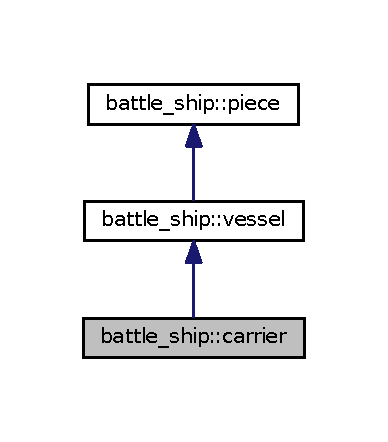
\includegraphics[width=186pt]{classbattle__ship_1_1carrier__inherit__graph}
\end{center}
\end{figure}


Collaboration diagram for battle\+\_\+ship\+:\+:carrier\+:
\nopagebreak
\begin{figure}[H]
\begin{center}
\leavevmode
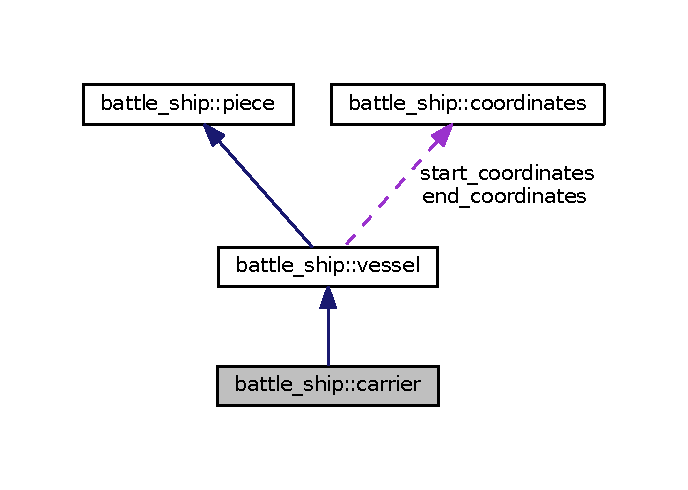
\includegraphics[width=330pt]{classbattle__ship_1_1carrier__coll__graph}
\end{center}
\end{figure}
\subsection*{Public Member Functions}
\begin{DoxyCompactItemize}
\item 
\hyperlink{classbattle__ship_1_1carrier_a9eaaa54c8884c25a1f99c397df789ca0}{carrier} ()=default
\item 
\hyperlink{classbattle__ship_1_1carrier_a3bb443575cd2f35ab21981b984c0fa02}{carrier} (\hyperlink{structbattle__ship_1_1coordinates}{coordinates} p, \hyperlink{namespacebattle__ship_aed87488f0a73f0d0679fe343fb61c784}{orientation} o)
\item 
\hyperlink{classbattle__ship_1_1carrier_a3642e56afffedbe7e20af863d0dde697}{$\sim$carrier} ()=default
\end{DoxyCompactItemize}
\subsection*{Additional Inherited Members}


\subsection{Detailed Description}


Definition at line 8 of file carrier.\+h.



\subsection{Constructor \& Destructor Documentation}
\mbox{\Hypertarget{classbattle__ship_1_1carrier_a9eaaa54c8884c25a1f99c397df789ca0}\label{classbattle__ship_1_1carrier_a9eaaa54c8884c25a1f99c397df789ca0}} 
\index{battle\+\_\+ship\+::carrier@{battle\+\_\+ship\+::carrier}!carrier@{carrier}}
\index{carrier@{carrier}!battle\+\_\+ship\+::carrier@{battle\+\_\+ship\+::carrier}}
\subsubsection{\texorpdfstring{carrier()}{carrier()}\hspace{0.1cm}{\footnotesize\ttfamily [1/2]}}
{\footnotesize\ttfamily battle\+\_\+ship\+::carrier\+::carrier (\begin{DoxyParamCaption}{ }\end{DoxyParamCaption})\hspace{0.3cm}{\ttfamily [default]}}

\mbox{\Hypertarget{classbattle__ship_1_1carrier_a3bb443575cd2f35ab21981b984c0fa02}\label{classbattle__ship_1_1carrier_a3bb443575cd2f35ab21981b984c0fa02}} 
\index{battle\+\_\+ship\+::carrier@{battle\+\_\+ship\+::carrier}!carrier@{carrier}}
\index{carrier@{carrier}!battle\+\_\+ship\+::carrier@{battle\+\_\+ship\+::carrier}}
\subsubsection{\texorpdfstring{carrier()}{carrier()}\hspace{0.1cm}{\footnotesize\ttfamily [2/2]}}
{\footnotesize\ttfamily battle\+\_\+ship\+::carrier\+::carrier (\begin{DoxyParamCaption}\item[{\hyperlink{structbattle__ship_1_1coordinates}{coordinates}}]{p,  }\item[{\hyperlink{namespacebattle__ship_aed87488f0a73f0d0679fe343fb61c784}{orientation}}]{o }\end{DoxyParamCaption})\hspace{0.3cm}{\ttfamily [inline]}}



Definition at line 12 of file carrier.\+h.

\mbox{\Hypertarget{classbattle__ship_1_1carrier_a3642e56afffedbe7e20af863d0dde697}\label{classbattle__ship_1_1carrier_a3642e56afffedbe7e20af863d0dde697}} 
\index{battle\+\_\+ship\+::carrier@{battle\+\_\+ship\+::carrier}!````~carrier@{$\sim$carrier}}
\index{````~carrier@{$\sim$carrier}!battle\+\_\+ship\+::carrier@{battle\+\_\+ship\+::carrier}}
\subsubsection{\texorpdfstring{$\sim$carrier()}{~carrier()}}
{\footnotesize\ttfamily battle\+\_\+ship\+::carrier\+::$\sim$carrier (\begin{DoxyParamCaption}{ }\end{DoxyParamCaption})\hspace{0.3cm}{\ttfamily [default]}}



The documentation for this class was generated from the following file\+:\begin{DoxyCompactItemize}
\item 
include/\hyperlink{carrier_8h}{carrier.\+h}\end{DoxyCompactItemize}

\hypertarget{structbattle__ship_1_1coordinates}{}\section{battle\+\_\+ship\+:\+:coordinates Struct Reference}
\label{structbattle__ship_1_1coordinates}\index{battle\+\_\+ship\+::coordinates@{battle\+\_\+ship\+::coordinates}}


{\ttfamily \#include $<$coordinates.\+h$>$}

\subsection*{Public Member Functions}
\begin{DoxyCompactItemize}
\item 
\hyperlink{structbattle__ship_1_1coordinates}{coordinates} \hyperlink{structbattle__ship_1_1coordinates_a2ab2b70ad53571e339c4c509547419c7}{boosted\+\_\+x} (std\+::size\+\_\+t length) const
\item 
\hyperlink{structbattle__ship_1_1coordinates}{coordinates} \hyperlink{structbattle__ship_1_1coordinates_af45f6a271dd7c5c97556d2593d455313}{boosted\+\_\+y} (std\+::size\+\_\+t width) const
\end{DoxyCompactItemize}
\subsection*{Public Attributes}
\begin{DoxyCompactItemize}
\item 
\hyperlink{namespacebattle__ship_ab3bfa90e413692dac2d4463364f80561}{x\+\_\+axis} \hyperlink{structbattle__ship_1_1coordinates_acda28ed24b163de319f6431762db3a72}{col}
\item 
std\+::size\+\_\+t \hyperlink{structbattle__ship_1_1coordinates_a436b0722a4b7244c5cbdcaefb2a76f0f}{row}
\end{DoxyCompactItemize}
\subsection*{Friends}
\begin{DoxyCompactItemize}
\item 
std\+::ostream \& \hyperlink{structbattle__ship_1_1coordinates_a3addd697b39df26c1807d744c30e65b5}{operator$<$$<$} (std\+::ostream \&os, const \hyperlink{structbattle__ship_1_1coordinates}{coordinates} \&p)
\item 
bool \hyperlink{structbattle__ship_1_1coordinates_afd9a944ba3ab08355a0ae36d35e57d85}{operator$>$$>$} (std\+::istream \&is, \hyperlink{structbattle__ship_1_1coordinates}{coordinates} \&p)
\end{DoxyCompactItemize}


\subsection{Detailed Description}


Definition at line 18 of file coordinates.\+h.



\subsection{Member Function Documentation}
\mbox{\Hypertarget{structbattle__ship_1_1coordinates_a2ab2b70ad53571e339c4c509547419c7}\label{structbattle__ship_1_1coordinates_a2ab2b70ad53571e339c4c509547419c7}} 
\index{battle\+\_\+ship\+::coordinates@{battle\+\_\+ship\+::coordinates}!boosted\+\_\+x@{boosted\+\_\+x}}
\index{boosted\+\_\+x@{boosted\+\_\+x}!battle\+\_\+ship\+::coordinates@{battle\+\_\+ship\+::coordinates}}
\subsubsection{\texorpdfstring{boosted\+\_\+x()}{boosted\_x()}}
{\footnotesize\ttfamily \hyperlink{structbattle__ship_1_1coordinates}{battle\+\_\+ship\+::coordinates} battle\+\_\+ship\+::coordinates\+::boosted\+\_\+x (\begin{DoxyParamCaption}\item[{std\+::size\+\_\+t}]{length }\end{DoxyParamCaption}) const}



Definition at line 46 of file coordinates.\+cpp.

\mbox{\Hypertarget{structbattle__ship_1_1coordinates_af45f6a271dd7c5c97556d2593d455313}\label{structbattle__ship_1_1coordinates_af45f6a271dd7c5c97556d2593d455313}} 
\index{battle\+\_\+ship\+::coordinates@{battle\+\_\+ship\+::coordinates}!boosted\+\_\+y@{boosted\+\_\+y}}
\index{boosted\+\_\+y@{boosted\+\_\+y}!battle\+\_\+ship\+::coordinates@{battle\+\_\+ship\+::coordinates}}
\subsubsection{\texorpdfstring{boosted\+\_\+y()}{boosted\_y()}}
{\footnotesize\ttfamily \hyperlink{structbattle__ship_1_1coordinates}{battle\+\_\+ship\+::coordinates} battle\+\_\+ship\+::coordinates\+::boosted\+\_\+y (\begin{DoxyParamCaption}\item[{std\+::size\+\_\+t}]{width }\end{DoxyParamCaption}) const}



Definition at line 51 of file coordinates.\+cpp.



\subsection{Friends And Related Function Documentation}
\mbox{\Hypertarget{structbattle__ship_1_1coordinates_a3addd697b39df26c1807d744c30e65b5}\label{structbattle__ship_1_1coordinates_a3addd697b39df26c1807d744c30e65b5}} 
\index{battle\+\_\+ship\+::coordinates@{battle\+\_\+ship\+::coordinates}!operator$<$$<$@{operator$<$$<$}}
\index{operator$<$$<$@{operator$<$$<$}!battle\+\_\+ship\+::coordinates@{battle\+\_\+ship\+::coordinates}}
\subsubsection{\texorpdfstring{operator$<$$<$}{operator<<}}
{\footnotesize\ttfamily std\+::ostream\& operator$<$$<$ (\begin{DoxyParamCaption}\item[{std\+::ostream \&}]{os,  }\item[{const \hyperlink{structbattle__ship_1_1coordinates}{coordinates} \&}]{p }\end{DoxyParamCaption})\hspace{0.3cm}{\ttfamily [friend]}}



Definition at line 8 of file coordinates.\+cpp.

\mbox{\Hypertarget{structbattle__ship_1_1coordinates_afd9a944ba3ab08355a0ae36d35e57d85}\label{structbattle__ship_1_1coordinates_afd9a944ba3ab08355a0ae36d35e57d85}} 
\index{battle\+\_\+ship\+::coordinates@{battle\+\_\+ship\+::coordinates}!operator$>$$>$@{operator$>$$>$}}
\index{operator$>$$>$@{operator$>$$>$}!battle\+\_\+ship\+::coordinates@{battle\+\_\+ship\+::coordinates}}
\subsubsection{\texorpdfstring{operator$>$$>$}{operator>>}}
{\footnotesize\ttfamily bool operator$>$$>$ (\begin{DoxyParamCaption}\item[{std\+::istream \&}]{is,  }\item[{\hyperlink{structbattle__ship_1_1coordinates}{coordinates} \&}]{p }\end{DoxyParamCaption})\hspace{0.3cm}{\ttfamily [friend]}}



Definition at line 15 of file coordinates.\+cpp.



\subsection{Member Data Documentation}
\mbox{\Hypertarget{structbattle__ship_1_1coordinates_acda28ed24b163de319f6431762db3a72}\label{structbattle__ship_1_1coordinates_acda28ed24b163de319f6431762db3a72}} 
\index{battle\+\_\+ship\+::coordinates@{battle\+\_\+ship\+::coordinates}!col@{col}}
\index{col@{col}!battle\+\_\+ship\+::coordinates@{battle\+\_\+ship\+::coordinates}}
\subsubsection{\texorpdfstring{col}{col}}
{\footnotesize\ttfamily \hyperlink{namespacebattle__ship_ab3bfa90e413692dac2d4463364f80561}{x\+\_\+axis} battle\+\_\+ship\+::coordinates\+::col}



Definition at line 21 of file coordinates.\+h.

\mbox{\Hypertarget{structbattle__ship_1_1coordinates_a436b0722a4b7244c5cbdcaefb2a76f0f}\label{structbattle__ship_1_1coordinates_a436b0722a4b7244c5cbdcaefb2a76f0f}} 
\index{battle\+\_\+ship\+::coordinates@{battle\+\_\+ship\+::coordinates}!row@{row}}
\index{row@{row}!battle\+\_\+ship\+::coordinates@{battle\+\_\+ship\+::coordinates}}
\subsubsection{\texorpdfstring{row}{row}}
{\footnotesize\ttfamily std\+::size\+\_\+t battle\+\_\+ship\+::coordinates\+::row}



Definition at line 22 of file coordinates.\+h.



The documentation for this struct was generated from the following files\+:\begin{DoxyCompactItemize}
\item 
include/\hyperlink{coordinates_8h}{coordinates.\+h}\item 
src/\hyperlink{coordinates_8cpp}{coordinates.\+cpp}\end{DoxyCompactItemize}

\hypertarget{classbattle__ship_1_1cruiser}{}\section{battle\+\_\+ship\+:\+:cruiser Class Reference}
\label{classbattle__ship_1_1cruiser}\index{battle\+\_\+ship\+::cruiser@{battle\+\_\+ship\+::cruiser}}


{\ttfamily \#include $<$cruiser.\+h$>$}



Inheritance diagram for battle\+\_\+ship\+:\+:cruiser\+:
\nopagebreak
\begin{figure}[H]
\begin{center}
\leavevmode
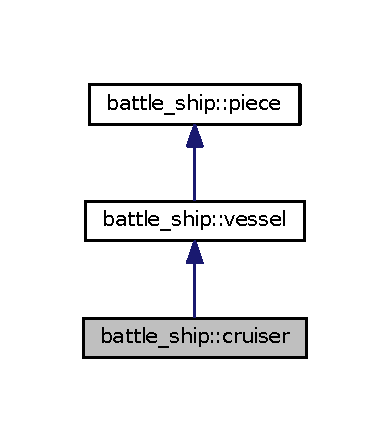
\includegraphics[width=187pt]{classbattle__ship_1_1cruiser__inherit__graph}
\end{center}
\end{figure}


Collaboration diagram for battle\+\_\+ship\+:\+:cruiser\+:
\nopagebreak
\begin{figure}[H]
\begin{center}
\leavevmode
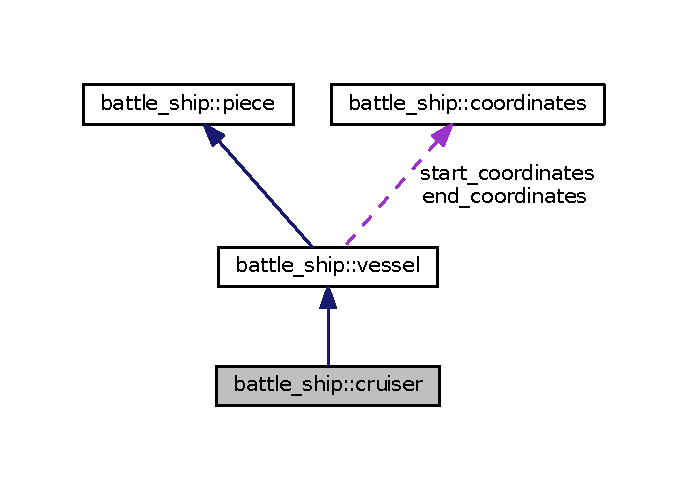
\includegraphics[width=330pt]{classbattle__ship_1_1cruiser__coll__graph}
\end{center}
\end{figure}
\subsection*{Public Member Functions}
\begin{DoxyCompactItemize}
\item 
\hyperlink{classbattle__ship_1_1cruiser_aa8fad74fb5caf3fd0cec5429b97fb46a}{cruiser} ()=default
\item 
\hyperlink{classbattle__ship_1_1cruiser_a3460b4b49152a6653122e30224114115}{cruiser} (\hyperlink{structbattle__ship_1_1coordinates}{coordinates} p, \hyperlink{namespacebattle__ship_aed87488f0a73f0d0679fe343fb61c784}{orientation} o)
\item 
\hyperlink{classbattle__ship_1_1cruiser_a78e3074b6331c963a2ba3200a14a85c3}{$\sim$cruiser} ()=default
\end{DoxyCompactItemize}
\subsection*{Additional Inherited Members}


\subsection{Detailed Description}


Definition at line 8 of file cruiser.\+h.



\subsection{Constructor \& Destructor Documentation}
\mbox{\Hypertarget{classbattle__ship_1_1cruiser_aa8fad74fb5caf3fd0cec5429b97fb46a}\label{classbattle__ship_1_1cruiser_aa8fad74fb5caf3fd0cec5429b97fb46a}} 
\index{battle\+\_\+ship\+::cruiser@{battle\+\_\+ship\+::cruiser}!cruiser@{cruiser}}
\index{cruiser@{cruiser}!battle\+\_\+ship\+::cruiser@{battle\+\_\+ship\+::cruiser}}
\subsubsection{\texorpdfstring{cruiser()}{cruiser()}\hspace{0.1cm}{\footnotesize\ttfamily [1/2]}}
{\footnotesize\ttfamily battle\+\_\+ship\+::cruiser\+::cruiser (\begin{DoxyParamCaption}{ }\end{DoxyParamCaption})\hspace{0.3cm}{\ttfamily [default]}}

\mbox{\Hypertarget{classbattle__ship_1_1cruiser_a3460b4b49152a6653122e30224114115}\label{classbattle__ship_1_1cruiser_a3460b4b49152a6653122e30224114115}} 
\index{battle\+\_\+ship\+::cruiser@{battle\+\_\+ship\+::cruiser}!cruiser@{cruiser}}
\index{cruiser@{cruiser}!battle\+\_\+ship\+::cruiser@{battle\+\_\+ship\+::cruiser}}
\subsubsection{\texorpdfstring{cruiser()}{cruiser()}\hspace{0.1cm}{\footnotesize\ttfamily [2/2]}}
{\footnotesize\ttfamily battle\+\_\+ship\+::cruiser\+::cruiser (\begin{DoxyParamCaption}\item[{\hyperlink{structbattle__ship_1_1coordinates}{coordinates}}]{p,  }\item[{\hyperlink{namespacebattle__ship_aed87488f0a73f0d0679fe343fb61c784}{orientation}}]{o }\end{DoxyParamCaption})\hspace{0.3cm}{\ttfamily [inline]}}



Definition at line 12 of file cruiser.\+h.

\mbox{\Hypertarget{classbattle__ship_1_1cruiser_a78e3074b6331c963a2ba3200a14a85c3}\label{classbattle__ship_1_1cruiser_a78e3074b6331c963a2ba3200a14a85c3}} 
\index{battle\+\_\+ship\+::cruiser@{battle\+\_\+ship\+::cruiser}!````~cruiser@{$\sim$cruiser}}
\index{````~cruiser@{$\sim$cruiser}!battle\+\_\+ship\+::cruiser@{battle\+\_\+ship\+::cruiser}}
\subsubsection{\texorpdfstring{$\sim$cruiser()}{~cruiser()}}
{\footnotesize\ttfamily battle\+\_\+ship\+::cruiser\+::$\sim$cruiser (\begin{DoxyParamCaption}{ }\end{DoxyParamCaption})\hspace{0.3cm}{\ttfamily [default]}}



The documentation for this class was generated from the following file\+:\begin{DoxyCompactItemize}
\item 
include/\hyperlink{cruiser_8h}{cruiser.\+h}\end{DoxyCompactItemize}

\hypertarget{classbattle__ship_1_1destroyer}{}\section{battle\+\_\+ship\+:\+:destroyer Class Reference}
\label{classbattle__ship_1_1destroyer}\index{battle\+\_\+ship\+::destroyer@{battle\+\_\+ship\+::destroyer}}


{\ttfamily \#include $<$destroyer.\+h$>$}



Inheritance diagram for battle\+\_\+ship\+:\+:destroyer\+:
\nopagebreak
\begin{figure}[H]
\begin{center}
\leavevmode
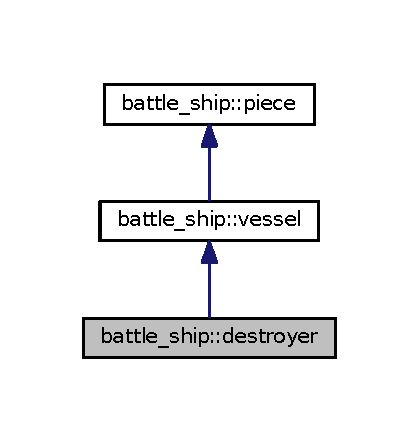
\includegraphics[width=201pt]{classbattle__ship_1_1destroyer__inherit__graph}
\end{center}
\end{figure}


Collaboration diagram for battle\+\_\+ship\+:\+:destroyer\+:
\nopagebreak
\begin{figure}[H]
\begin{center}
\leavevmode
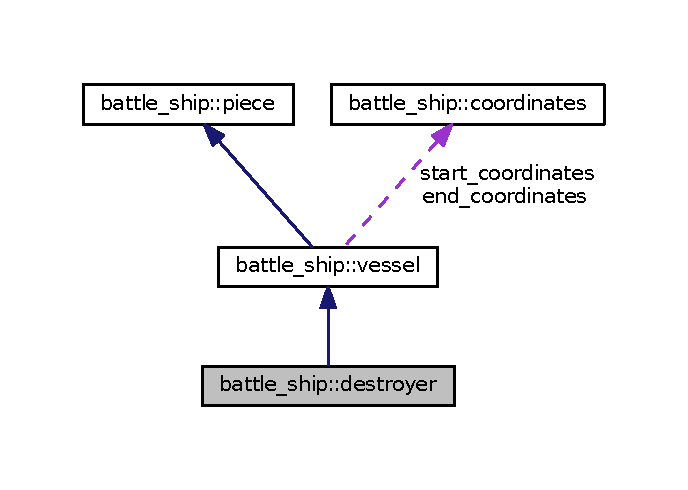
\includegraphics[width=330pt]{classbattle__ship_1_1destroyer__coll__graph}
\end{center}
\end{figure}
\subsection*{Public Member Functions}
\begin{DoxyCompactItemize}
\item 
\hyperlink{classbattle__ship_1_1destroyer_ae26647f7b12b2dc4cc1ef6951734a08b}{destroyer} ()=default
\item 
\hyperlink{classbattle__ship_1_1destroyer_af0f630a4ecc4d6667b6adf021633da83}{destroyer} (\hyperlink{structbattle__ship_1_1coordinates}{coordinates} p, \hyperlink{namespacebattle__ship_aed87488f0a73f0d0679fe343fb61c784}{orientation} o)
\item 
\hyperlink{classbattle__ship_1_1destroyer_a6abbf5c8970c69703ae57786e2247f9a}{$\sim$destroyer} ()=default
\end{DoxyCompactItemize}
\subsection*{Additional Inherited Members}


\subsection{Detailed Description}


Definition at line 8 of file destroyer.\+h.



\subsection{Constructor \& Destructor Documentation}
\mbox{\Hypertarget{classbattle__ship_1_1destroyer_ae26647f7b12b2dc4cc1ef6951734a08b}\label{classbattle__ship_1_1destroyer_ae26647f7b12b2dc4cc1ef6951734a08b}} 
\index{battle\+\_\+ship\+::destroyer@{battle\+\_\+ship\+::destroyer}!destroyer@{destroyer}}
\index{destroyer@{destroyer}!battle\+\_\+ship\+::destroyer@{battle\+\_\+ship\+::destroyer}}
\subsubsection{\texorpdfstring{destroyer()}{destroyer()}\hspace{0.1cm}{\footnotesize\ttfamily [1/2]}}
{\footnotesize\ttfamily battle\+\_\+ship\+::destroyer\+::destroyer (\begin{DoxyParamCaption}{ }\end{DoxyParamCaption})\hspace{0.3cm}{\ttfamily [default]}}

\mbox{\Hypertarget{classbattle__ship_1_1destroyer_af0f630a4ecc4d6667b6adf021633da83}\label{classbattle__ship_1_1destroyer_af0f630a4ecc4d6667b6adf021633da83}} 
\index{battle\+\_\+ship\+::destroyer@{battle\+\_\+ship\+::destroyer}!destroyer@{destroyer}}
\index{destroyer@{destroyer}!battle\+\_\+ship\+::destroyer@{battle\+\_\+ship\+::destroyer}}
\subsubsection{\texorpdfstring{destroyer()}{destroyer()}\hspace{0.1cm}{\footnotesize\ttfamily [2/2]}}
{\footnotesize\ttfamily battle\+\_\+ship\+::destroyer\+::destroyer (\begin{DoxyParamCaption}\item[{\hyperlink{structbattle__ship_1_1coordinates}{coordinates}}]{p,  }\item[{\hyperlink{namespacebattle__ship_aed87488f0a73f0d0679fe343fb61c784}{orientation}}]{o }\end{DoxyParamCaption})\hspace{0.3cm}{\ttfamily [inline]}}



Definition at line 12 of file destroyer.\+h.

\mbox{\Hypertarget{classbattle__ship_1_1destroyer_a6abbf5c8970c69703ae57786e2247f9a}\label{classbattle__ship_1_1destroyer_a6abbf5c8970c69703ae57786e2247f9a}} 
\index{battle\+\_\+ship\+::destroyer@{battle\+\_\+ship\+::destroyer}!````~destroyer@{$\sim$destroyer}}
\index{````~destroyer@{$\sim$destroyer}!battle\+\_\+ship\+::destroyer@{battle\+\_\+ship\+::destroyer}}
\subsubsection{\texorpdfstring{$\sim$destroyer()}{~destroyer()}}
{\footnotesize\ttfamily battle\+\_\+ship\+::destroyer\+::$\sim$destroyer (\begin{DoxyParamCaption}{ }\end{DoxyParamCaption})\hspace{0.3cm}{\ttfamily [default]}}



The documentation for this class was generated from the following file\+:\begin{DoxyCompactItemize}
\item 
include/\hyperlink{destroyer_8h}{destroyer.\+h}\end{DoxyCompactItemize}

\hypertarget{classbattle__ship_1_1game}{}\section{battle\+\_\+ship\+:\+:game Class Reference}
\label{classbattle__ship_1_1game}\index{battle\+\_\+ship\+::game@{battle\+\_\+ship\+::game}}


Holds the current battle state.  




{\ttfamily \#include $<$game.\+h$>$}

\subsection*{Public Member Functions}
\begin{DoxyCompactItemize}
\item 
\hyperlink{classbattle__ship_1_1game_a3a98cd01dec3c29d91d057049c421c89}{game} ()=default
\item 
\hyperlink{classbattle__ship_1_1game_a932962ce40fffb1c8008a353971afa4c}{game} (size\+\_\+t starting\+\_\+turn, std\+::shared\+\_\+ptr$<$ \hyperlink{classbattle__ship_1_1player}{player} $>$ p1, std\+::shared\+\_\+ptr$<$ \hyperlink{classbattle__ship_1_1player}{player} $>$ p2)
\item 
\hyperlink{classbattle__ship_1_1player}{player} \& \hyperlink{classbattle__ship_1_1game_a6a93475d1fae5c83ae58182376f1292c}{get\+\_\+player} (size\+\_\+t p)
\item 
void \hyperlink{classbattle__ship_1_1game_a0e5a85f6c1f0cff5e1104545b5222026}{toggle\+\_\+turn} ()
\item 
void \hyperlink{classbattle__ship_1_1game_a8bd311ac1aaab0a16c06b4f1b9664af4}{play} (std\+::shared\+\_\+ptr$<$ \hyperlink{classbattle__ship_1_1player}{player} $>$ \&winner)
\item 
bool \hyperlink{classbattle__ship_1_1game_a2f6eceb02db97507f52e08c1dafcf5e4}{has\+\_\+player\+\_\+lost} (\hyperlink{classbattle__ship_1_1player}{player} \&p)
\item 
\hyperlink{classbattle__ship_1_1game_aa95dac5c30c567ae407a3b67ceae324d}{$\sim$game} ()=default
\end{DoxyCompactItemize}


\subsection{Detailed Description}
Holds the current battle state. 

\begin{DoxyAuthor}{Author}
Enrico Zammit Lonardelli
\end{DoxyAuthor}
This class controls the logic of taking turns and holds state about each player. Also holds the logic to check whether end game conditions have been met

Contact\+: \href{mailto:enrico.zammitl@gmail.com}{\tt enrico.\+zammitl@gmail.\+com}

Created on\+: Sat, 11 Apr 2020 09\+:49\+:03 

Definition at line 20 of file game.\+h.



\subsection{Constructor \& Destructor Documentation}
\mbox{\Hypertarget{classbattle__ship_1_1game_a3a98cd01dec3c29d91d057049c421c89}\label{classbattle__ship_1_1game_a3a98cd01dec3c29d91d057049c421c89}} 
\index{battle\+\_\+ship\+::game@{battle\+\_\+ship\+::game}!game@{game}}
\index{game@{game}!battle\+\_\+ship\+::game@{battle\+\_\+ship\+::game}}
\subsubsection{\texorpdfstring{game()}{game()}\hspace{0.1cm}{\footnotesize\ttfamily [1/2]}}
{\footnotesize\ttfamily battle\+\_\+ship\+::game\+::game (\begin{DoxyParamCaption}{ }\end{DoxyParamCaption})\hspace{0.3cm}{\ttfamily [default]}}

\mbox{\Hypertarget{classbattle__ship_1_1game_a932962ce40fffb1c8008a353971afa4c}\label{classbattle__ship_1_1game_a932962ce40fffb1c8008a353971afa4c}} 
\index{battle\+\_\+ship\+::game@{battle\+\_\+ship\+::game}!game@{game}}
\index{game@{game}!battle\+\_\+ship\+::game@{battle\+\_\+ship\+::game}}
\subsubsection{\texorpdfstring{game()}{game()}\hspace{0.1cm}{\footnotesize\ttfamily [2/2]}}
{\footnotesize\ttfamily battle\+\_\+ship\+::game\+::game (\begin{DoxyParamCaption}\item[{size\+\_\+t}]{starting\+\_\+turn,  }\item[{std\+::shared\+\_\+ptr$<$ \hyperlink{classbattle__ship_1_1player}{player} $>$}]{p1,  }\item[{std\+::shared\+\_\+ptr$<$ \hyperlink{classbattle__ship_1_1player}{player} $>$}]{p2 }\end{DoxyParamCaption})\hspace{0.3cm}{\ttfamily [inline]}}



Definition at line 28 of file game.\+h.

\mbox{\Hypertarget{classbattle__ship_1_1game_aa95dac5c30c567ae407a3b67ceae324d}\label{classbattle__ship_1_1game_aa95dac5c30c567ae407a3b67ceae324d}} 
\index{battle\+\_\+ship\+::game@{battle\+\_\+ship\+::game}!````~game@{$\sim$game}}
\index{````~game@{$\sim$game}!battle\+\_\+ship\+::game@{battle\+\_\+ship\+::game}}
\subsubsection{\texorpdfstring{$\sim$game()}{~game()}}
{\footnotesize\ttfamily battle\+\_\+ship\+::game\+::$\sim$game (\begin{DoxyParamCaption}{ }\end{DoxyParamCaption})\hspace{0.3cm}{\ttfamily [default]}}



\subsection{Member Function Documentation}
\mbox{\Hypertarget{classbattle__ship_1_1game_a6a93475d1fae5c83ae58182376f1292c}\label{classbattle__ship_1_1game_a6a93475d1fae5c83ae58182376f1292c}} 
\index{battle\+\_\+ship\+::game@{battle\+\_\+ship\+::game}!get\+\_\+player@{get\+\_\+player}}
\index{get\+\_\+player@{get\+\_\+player}!battle\+\_\+ship\+::game@{battle\+\_\+ship\+::game}}
\subsubsection{\texorpdfstring{get\+\_\+player()}{get\_player()}}
{\footnotesize\ttfamily \hyperlink{classbattle__ship_1_1player}{battle\+\_\+ship\+::player} \& battle\+\_\+ship\+::game\+::get\+\_\+player (\begin{DoxyParamCaption}\item[{size\+\_\+t}]{p }\end{DoxyParamCaption})}



Definition at line 8 of file game.\+cpp.

\mbox{\Hypertarget{classbattle__ship_1_1game_a2f6eceb02db97507f52e08c1dafcf5e4}\label{classbattle__ship_1_1game_a2f6eceb02db97507f52e08c1dafcf5e4}} 
\index{battle\+\_\+ship\+::game@{battle\+\_\+ship\+::game}!has\+\_\+player\+\_\+lost@{has\+\_\+player\+\_\+lost}}
\index{has\+\_\+player\+\_\+lost@{has\+\_\+player\+\_\+lost}!battle\+\_\+ship\+::game@{battle\+\_\+ship\+::game}}
\subsubsection{\texorpdfstring{has\+\_\+player\+\_\+lost()}{has\_player\_lost()}}
{\footnotesize\ttfamily bool battle\+\_\+ship\+::game\+::has\+\_\+player\+\_\+lost (\begin{DoxyParamCaption}\item[{\hyperlink{classbattle__ship_1_1player}{battle\+\_\+ship\+::player} \&}]{p }\end{DoxyParamCaption})}



Definition at line 63 of file game.\+cpp.

\mbox{\Hypertarget{classbattle__ship_1_1game_a8bd311ac1aaab0a16c06b4f1b9664af4}\label{classbattle__ship_1_1game_a8bd311ac1aaab0a16c06b4f1b9664af4}} 
\index{battle\+\_\+ship\+::game@{battle\+\_\+ship\+::game}!play@{play}}
\index{play@{play}!battle\+\_\+ship\+::game@{battle\+\_\+ship\+::game}}
\subsubsection{\texorpdfstring{play()}{play()}}
{\footnotesize\ttfamily void battle\+\_\+ship\+::game\+::play (\begin{DoxyParamCaption}\item[{std\+::shared\+\_\+ptr$<$ \hyperlink{classbattle__ship_1_1player}{player} $>$ \&}]{winner }\end{DoxyParamCaption})}



Definition at line 20 of file game.\+cpp.

\mbox{\Hypertarget{classbattle__ship_1_1game_a0e5a85f6c1f0cff5e1104545b5222026}\label{classbattle__ship_1_1game_a0e5a85f6c1f0cff5e1104545b5222026}} 
\index{battle\+\_\+ship\+::game@{battle\+\_\+ship\+::game}!toggle\+\_\+turn@{toggle\+\_\+turn}}
\index{toggle\+\_\+turn@{toggle\+\_\+turn}!battle\+\_\+ship\+::game@{battle\+\_\+ship\+::game}}
\subsubsection{\texorpdfstring{toggle\+\_\+turn()}{toggle\_turn()}}
{\footnotesize\ttfamily void battle\+\_\+ship\+::game\+::toggle\+\_\+turn (\begin{DoxyParamCaption}{ }\end{DoxyParamCaption})\hspace{0.3cm}{\ttfamily [inline]}}



Definition at line 35 of file game.\+h.



The documentation for this class was generated from the following files\+:\begin{DoxyCompactItemize}
\item 
include/\hyperlink{game_8h}{game.\+h}\item 
src/\hyperlink{game_8cpp}{game.\+cpp}\end{DoxyCompactItemize}

\hypertarget{classbattle__ship_1_1geometry}{}\section{battle\+\_\+ship\+:\+:geometry Class Reference}
\label{classbattle__ship_1_1geometry}\index{battle\+\_\+ship\+::geometry@{battle\+\_\+ship\+::geometry}}


{\ttfamily \#include $<$geometry.\+h$>$}

\subsection*{Static Public Member Functions}
\begin{DoxyCompactItemize}
\item 
static int \hyperlink{classbattle__ship_1_1geometry_abe15f3d75f562cb7f67f0facfad73628}{orientation} (\hyperlink{structbattle__ship_1_1coordinates}{battle\+\_\+ship\+::coordinates} p, \hyperlink{structbattle__ship_1_1coordinates}{battle\+\_\+ship\+::coordinates} q, \hyperlink{structbattle__ship_1_1coordinates}{battle\+\_\+ship\+::coordinates} r)
\item 
static bool \hyperlink{classbattle__ship_1_1geometry_ac6ab7fe7ccaeca7e7c0df8c0ebdbbce4}{on\+\_\+segment} (\hyperlink{structbattle__ship_1_1coordinates}{battle\+\_\+ship\+::coordinates} p, \hyperlink{structbattle__ship_1_1coordinates}{battle\+\_\+ship\+::coordinates} q, \hyperlink{structbattle__ship_1_1coordinates}{battle\+\_\+ship\+::coordinates} r)
\item 
static bool \hyperlink{classbattle__ship_1_1geometry_a8ed3083520abd281bf2c36568affb245}{do\+\_\+intersect} (\hyperlink{structbattle__ship_1_1coordinates}{battle\+\_\+ship\+::coordinates} start\+\_\+1, \hyperlink{structbattle__ship_1_1coordinates}{battle\+\_\+ship\+::coordinates} end\+\_\+1, \hyperlink{structbattle__ship_1_1coordinates}{battle\+\_\+ship\+::coordinates} start\+\_\+2, \hyperlink{structbattle__ship_1_1coordinates}{battle\+\_\+ship\+::coordinates} end\+\_\+2)
\end{DoxyCompactItemize}


\subsection{Detailed Description}


Definition at line 6 of file geometry.\+h.



\subsection{Member Function Documentation}
\mbox{\Hypertarget{classbattle__ship_1_1geometry_a8ed3083520abd281bf2c36568affb245}\label{classbattle__ship_1_1geometry_a8ed3083520abd281bf2c36568affb245}} 
\index{battle\+\_\+ship\+::geometry@{battle\+\_\+ship\+::geometry}!do\+\_\+intersect@{do\+\_\+intersect}}
\index{do\+\_\+intersect@{do\+\_\+intersect}!battle\+\_\+ship\+::geometry@{battle\+\_\+ship\+::geometry}}
\subsubsection{\texorpdfstring{do\+\_\+intersect()}{do\_intersect()}}
{\footnotesize\ttfamily bool battle\+\_\+ship\+::geometry\+::do\+\_\+intersect (\begin{DoxyParamCaption}\item[{\hyperlink{structbattle__ship_1_1coordinates}{battle\+\_\+ship\+::coordinates}}]{start\+\_\+1,  }\item[{\hyperlink{structbattle__ship_1_1coordinates}{battle\+\_\+ship\+::coordinates}}]{end\+\_\+1,  }\item[{\hyperlink{structbattle__ship_1_1coordinates}{battle\+\_\+ship\+::coordinates}}]{start\+\_\+2,  }\item[{\hyperlink{structbattle__ship_1_1coordinates}{battle\+\_\+ship\+::coordinates}}]{end\+\_\+2 }\end{DoxyParamCaption})\hspace{0.3cm}{\ttfamily [static]}}



Definition at line 31 of file geometry.\+cpp.

\mbox{\Hypertarget{classbattle__ship_1_1geometry_ac6ab7fe7ccaeca7e7c0df8c0ebdbbce4}\label{classbattle__ship_1_1geometry_ac6ab7fe7ccaeca7e7c0df8c0ebdbbce4}} 
\index{battle\+\_\+ship\+::geometry@{battle\+\_\+ship\+::geometry}!on\+\_\+segment@{on\+\_\+segment}}
\index{on\+\_\+segment@{on\+\_\+segment}!battle\+\_\+ship\+::geometry@{battle\+\_\+ship\+::geometry}}
\subsubsection{\texorpdfstring{on\+\_\+segment()}{on\_segment()}}
{\footnotesize\ttfamily bool battle\+\_\+ship\+::geometry\+::on\+\_\+segment (\begin{DoxyParamCaption}\item[{\hyperlink{structbattle__ship_1_1coordinates}{battle\+\_\+ship\+::coordinates}}]{p,  }\item[{\hyperlink{structbattle__ship_1_1coordinates}{battle\+\_\+ship\+::coordinates}}]{q,  }\item[{\hyperlink{structbattle__ship_1_1coordinates}{battle\+\_\+ship\+::coordinates}}]{r }\end{DoxyParamCaption})\hspace{0.3cm}{\ttfamily [static]}}



Definition at line 5 of file geometry.\+cpp.

\mbox{\Hypertarget{classbattle__ship_1_1geometry_abe15f3d75f562cb7f67f0facfad73628}\label{classbattle__ship_1_1geometry_abe15f3d75f562cb7f67f0facfad73628}} 
\index{battle\+\_\+ship\+::geometry@{battle\+\_\+ship\+::geometry}!orientation@{orientation}}
\index{orientation@{orientation}!battle\+\_\+ship\+::geometry@{battle\+\_\+ship\+::geometry}}
\subsubsection{\texorpdfstring{orientation()}{orientation()}}
{\footnotesize\ttfamily int battle\+\_\+ship\+::geometry\+::orientation (\begin{DoxyParamCaption}\item[{\hyperlink{structbattle__ship_1_1coordinates}{battle\+\_\+ship\+::coordinates}}]{p,  }\item[{\hyperlink{structbattle__ship_1_1coordinates}{battle\+\_\+ship\+::coordinates}}]{q,  }\item[{\hyperlink{structbattle__ship_1_1coordinates}{battle\+\_\+ship\+::coordinates}}]{r }\end{DoxyParamCaption})\hspace{0.3cm}{\ttfamily [static]}}



Definition at line 16 of file geometry.\+cpp.



The documentation for this class was generated from the following files\+:\begin{DoxyCompactItemize}
\item 
include/\hyperlink{geometry_8h}{geometry.\+h}\item 
src/\hyperlink{geometry_8cpp}{geometry.\+cpp}\end{DoxyCompactItemize}

\hypertarget{classbattle__ship_1_1highscore__manager}{}\section{battle\+\_\+ship\+:\+:highscore\+\_\+manager Class Reference}
\label{classbattle__ship_1_1highscore__manager}\index{battle\+\_\+ship\+::highscore\+\_\+manager@{battle\+\_\+ship\+::highscore\+\_\+manager}}


{\ttfamily \#include $<$highscore\+\_\+manager.\+h$>$}

\subsection*{Static Public Member Functions}
\begin{DoxyCompactItemize}
\item 
static void \hyperlink{classbattle__ship_1_1highscore__manager_a7fcb9a8ba8457ee9d66349d3f4c51fee}{add\+\_\+highscore} (std\+::tuple$<$ std\+::string, int $>$ h)
\item 
static void \hyperlink{classbattle__ship_1_1highscore__manager_a404a994ea85111522a7a4f571bcbacdc}{initialise\+\_\+highscores} ()
\end{DoxyCompactItemize}
\subsection*{Static Public Attributes}
\begin{DoxyCompactItemize}
\item 
static std\+::vector$<$ std\+::tuple$<$ std\+::string, int $>$ $>$ \hyperlink{classbattle__ship_1_1highscore__manager_a53bb0aa2445ba4caa4cfe7c4b0fef663}{all\+\_\+highscores}
\end{DoxyCompactItemize}


\subsection{Detailed Description}


Definition at line 8 of file highscore\+\_\+manager.\+h.



\subsection{Member Function Documentation}
\mbox{\Hypertarget{classbattle__ship_1_1highscore__manager_a7fcb9a8ba8457ee9d66349d3f4c51fee}\label{classbattle__ship_1_1highscore__manager_a7fcb9a8ba8457ee9d66349d3f4c51fee}} 
\index{battle\+\_\+ship\+::highscore\+\_\+manager@{battle\+\_\+ship\+::highscore\+\_\+manager}!add\+\_\+highscore@{add\+\_\+highscore}}
\index{add\+\_\+highscore@{add\+\_\+highscore}!battle\+\_\+ship\+::highscore\+\_\+manager@{battle\+\_\+ship\+::highscore\+\_\+manager}}
\subsubsection{\texorpdfstring{add\+\_\+highscore()}{add\_highscore()}}
{\footnotesize\ttfamily void battle\+\_\+ship\+::highscore\+\_\+manager\+::add\+\_\+highscore (\begin{DoxyParamCaption}\item[{std\+::tuple$<$ std\+::string, int $>$}]{h }\end{DoxyParamCaption})\hspace{0.3cm}{\ttfamily [static]}}



Definition at line 24 of file highscore\+\_\+manager.\+cpp.

\mbox{\Hypertarget{classbattle__ship_1_1highscore__manager_a404a994ea85111522a7a4f571bcbacdc}\label{classbattle__ship_1_1highscore__manager_a404a994ea85111522a7a4f571bcbacdc}} 
\index{battle\+\_\+ship\+::highscore\+\_\+manager@{battle\+\_\+ship\+::highscore\+\_\+manager}!initialise\+\_\+highscores@{initialise\+\_\+highscores}}
\index{initialise\+\_\+highscores@{initialise\+\_\+highscores}!battle\+\_\+ship\+::highscore\+\_\+manager@{battle\+\_\+ship\+::highscore\+\_\+manager}}
\subsubsection{\texorpdfstring{initialise\+\_\+highscores()}{initialise\_highscores()}}
{\footnotesize\ttfamily void battle\+\_\+ship\+::highscore\+\_\+manager\+::initialise\+\_\+highscores (\begin{DoxyParamCaption}{ }\end{DoxyParamCaption})\hspace{0.3cm}{\ttfamily [static]}}



Definition at line 11 of file highscore\+\_\+manager.\+cpp.



\subsection{Member Data Documentation}
\mbox{\Hypertarget{classbattle__ship_1_1highscore__manager_a53bb0aa2445ba4caa4cfe7c4b0fef663}\label{classbattle__ship_1_1highscore__manager_a53bb0aa2445ba4caa4cfe7c4b0fef663}} 
\index{battle\+\_\+ship\+::highscore\+\_\+manager@{battle\+\_\+ship\+::highscore\+\_\+manager}!all\+\_\+highscores@{all\+\_\+highscores}}
\index{all\+\_\+highscores@{all\+\_\+highscores}!battle\+\_\+ship\+::highscore\+\_\+manager@{battle\+\_\+ship\+::highscore\+\_\+manager}}
\subsubsection{\texorpdfstring{all\+\_\+highscores}{all\_highscores}}
{\footnotesize\ttfamily std\+::vector$<$ std\+::tuple$<$ std\+::string, int $>$ $>$ battle\+\_\+ship\+::highscore\+\_\+manager\+::all\+\_\+highscores\hspace{0.3cm}{\ttfamily [static]}}



Definition at line 10 of file highscore\+\_\+manager.\+h.



The documentation for this class was generated from the following files\+:\begin{DoxyCompactItemize}
\item 
include/\hyperlink{highscore__manager_8h}{highscore\+\_\+manager.\+h}\item 
src/\hyperlink{highscore__manager_8cpp}{highscore\+\_\+manager.\+cpp}\end{DoxyCompactItemize}

\hypertarget{classbattle__ship_1_1human}{}\section{battle\+\_\+ship\+:\+:human Class Reference}
\label{classbattle__ship_1_1human}\index{battle\+\_\+ship\+::human@{battle\+\_\+ship\+::human}}


A type of player Implements methods targeted for playable characters (human controlled)  




{\ttfamily \#include $<$human.\+h$>$}



Inheritance diagram for battle\+\_\+ship\+:\+:human\+:
\nopagebreak
\begin{figure}[H]
\begin{center}
\leavevmode
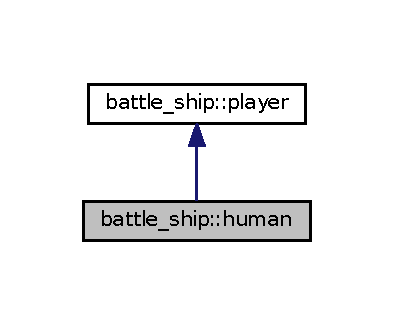
\includegraphics[width=179pt]{classbattle__ship_1_1human__inherit__graph}
\end{center}
\end{figure}


Collaboration diagram for battle\+\_\+ship\+:\+:human\+:
\nopagebreak
\begin{figure}[H]
\begin{center}
\leavevmode
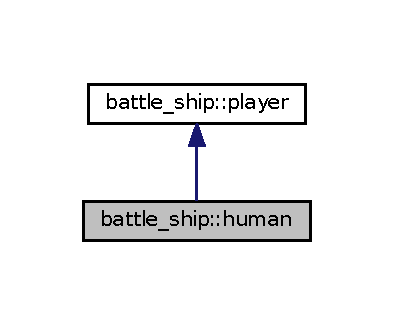
\includegraphics[width=179pt]{classbattle__ship_1_1human__coll__graph}
\end{center}
\end{figure}
\subsection*{Public Member Functions}
\begin{DoxyCompactItemize}
\item 
\hyperlink{classbattle__ship_1_1human_abf9adbf70e2b5cec288c900f337f4c56}{human} ()=default
\item 
\hyperlink{classbattle__ship_1_1human_a9d8abd36c22aeddad8c57a5b1e74b4cd}{human} (std\+::string uname, size\+\_\+t high, size\+\_\+t pass=0)
\item 
size\+\_\+t \hyperlink{classbattle__ship_1_1human_ac3529c252376938ce6b62ac40f8df3b3}{get\+\_\+highscore} ()
\item 
void \hyperlink{classbattle__ship_1_1human_a5b7e6cad4d1f187907a205b767a2fd7d}{save\+\_\+highscore} (size\+\_\+t h)
\item 
void \hyperlink{classbattle__ship_1_1human_ab6e8f18828d7671bbc7645f38369d370}{modify\+\_\+fleet} ()
\item 
void \hyperlink{classbattle__ship_1_1human_a3d14bca9009f7cfb8d4501d428524416}{save\+\_\+fleet} ()
\item 
bool \hyperlink{classbattle__ship_1_1human_adaea883b2eb5fa5932a9d7239c90bfd6}{add\+\_\+piece} ()
\item 
bool \hyperlink{classbattle__ship_1_1human_a2638497165f4a593b3b597a785fc3ee0}{remove\+\_\+piece} ()
\item 
bool \hyperlink{classbattle__ship_1_1human_a8f0addc975b597a92d4c82849c2fff5d}{edit\+\_\+piece} ()
\item 
void \hyperlink{classbattle__ship_1_1human_a583d0a9dd05c16f700d0d1825916faa3}{winning\+\_\+line} ()
\item 
void \hyperlink{classbattle__ship_1_1human_ad89701f0c4dd688c564b14a015059386}{attack} (\hyperlink{classbattle__ship_1_1piece}{piece} \&attacking\+\_\+piece, \hyperlink{classbattle__ship_1_1player}{player} \&\hyperlink{classbattle__ship_1_1player_af01292346caaf209039b6490ae18d8aa}{enemy})
\item 
\hyperlink{classbattle__ship_1_1human_ad1c94c01291be1e1908301cffc41497d}{$\sim$human} ()=default
\end{DoxyCompactItemize}
\subsection*{Additional Inherited Members}


\subsection{Detailed Description}
A type of player Implements methods targeted for playable characters (human controlled) 

\begin{DoxyAuthor}{Author}
Enrico Zammit Lonardelli
\end{DoxyAuthor}
Contact\+: \href{mailto:enrico.zammitl@gmail.com}{\tt enrico.\+zammitl@gmail.\+com}

Created on\+: Wed, 15 Apr 2020 17\+:55\+:28 

Definition at line 17 of file human.\+h.



\subsection{Constructor \& Destructor Documentation}
\mbox{\Hypertarget{classbattle__ship_1_1human_abf9adbf70e2b5cec288c900f337f4c56}\label{classbattle__ship_1_1human_abf9adbf70e2b5cec288c900f337f4c56}} 
\index{battle\+\_\+ship\+::human@{battle\+\_\+ship\+::human}!human@{human}}
\index{human@{human}!battle\+\_\+ship\+::human@{battle\+\_\+ship\+::human}}
\subsubsection{\texorpdfstring{human()}{human()}\hspace{0.1cm}{\footnotesize\ttfamily [1/2]}}
{\footnotesize\ttfamily battle\+\_\+ship\+::human\+::human (\begin{DoxyParamCaption}{ }\end{DoxyParamCaption})\hspace{0.3cm}{\ttfamily [default]}}

\mbox{\Hypertarget{classbattle__ship_1_1human_a9d8abd36c22aeddad8c57a5b1e74b4cd}\label{classbattle__ship_1_1human_a9d8abd36c22aeddad8c57a5b1e74b4cd}} 
\index{battle\+\_\+ship\+::human@{battle\+\_\+ship\+::human}!human@{human}}
\index{human@{human}!battle\+\_\+ship\+::human@{battle\+\_\+ship\+::human}}
\subsubsection{\texorpdfstring{human()}{human()}\hspace{0.1cm}{\footnotesize\ttfamily [2/2]}}
{\footnotesize\ttfamily battle\+\_\+ship\+::human\+::human (\begin{DoxyParamCaption}\item[{std\+::string}]{uname,  }\item[{size\+\_\+t}]{high,  }\item[{size\+\_\+t}]{pass = {\ttfamily 0} }\end{DoxyParamCaption})\hspace{0.3cm}{\ttfamily [inline]}}



Definition at line 24 of file human.\+h.

\mbox{\Hypertarget{classbattle__ship_1_1human_ad1c94c01291be1e1908301cffc41497d}\label{classbattle__ship_1_1human_ad1c94c01291be1e1908301cffc41497d}} 
\index{battle\+\_\+ship\+::human@{battle\+\_\+ship\+::human}!````~human@{$\sim$human}}
\index{````~human@{$\sim$human}!battle\+\_\+ship\+::human@{battle\+\_\+ship\+::human}}
\subsubsection{\texorpdfstring{$\sim$human()}{~human()}}
{\footnotesize\ttfamily battle\+\_\+ship\+::human\+::$\sim$human (\begin{DoxyParamCaption}{ }\end{DoxyParamCaption})\hspace{0.3cm}{\ttfamily [default]}}



\subsection{Member Function Documentation}
\mbox{\Hypertarget{classbattle__ship_1_1human_adaea883b2eb5fa5932a9d7239c90bfd6}\label{classbattle__ship_1_1human_adaea883b2eb5fa5932a9d7239c90bfd6}} 
\index{battle\+\_\+ship\+::human@{battle\+\_\+ship\+::human}!add\+\_\+piece@{add\+\_\+piece}}
\index{add\+\_\+piece@{add\+\_\+piece}!battle\+\_\+ship\+::human@{battle\+\_\+ship\+::human}}
\subsubsection{\texorpdfstring{add\+\_\+piece()}{add\_piece()}}
{\footnotesize\ttfamily bool battle\+\_\+ship\+::human\+::add\+\_\+piece (\begin{DoxyParamCaption}{ }\end{DoxyParamCaption})}



Definition at line 78 of file human.\+cpp.

\mbox{\Hypertarget{classbattle__ship_1_1human_ad89701f0c4dd688c564b14a015059386}\label{classbattle__ship_1_1human_ad89701f0c4dd688c564b14a015059386}} 
\index{battle\+\_\+ship\+::human@{battle\+\_\+ship\+::human}!attack@{attack}}
\index{attack@{attack}!battle\+\_\+ship\+::human@{battle\+\_\+ship\+::human}}
\subsubsection{\texorpdfstring{attack()}{attack()}}
{\footnotesize\ttfamily void battle\+\_\+ship\+::human\+::attack (\begin{DoxyParamCaption}\item[{\hyperlink{classbattle__ship_1_1piece}{battle\+\_\+ship\+::piece} \&}]{attacking\+\_\+piece,  }\item[{\hyperlink{classbattle__ship_1_1player}{battle\+\_\+ship\+::player} \&}]{enemy }\end{DoxyParamCaption})\hspace{0.3cm}{\ttfamily [virtual]}}



Implements \hyperlink{classbattle__ship_1_1player_a86be2256620cd5e20da6db7be8afdbc8}{battle\+\_\+ship\+::player}.



Definition at line 195 of file human.\+cpp.

\mbox{\Hypertarget{classbattle__ship_1_1human_a8f0addc975b597a92d4c82849c2fff5d}\label{classbattle__ship_1_1human_a8f0addc975b597a92d4c82849c2fff5d}} 
\index{battle\+\_\+ship\+::human@{battle\+\_\+ship\+::human}!edit\+\_\+piece@{edit\+\_\+piece}}
\index{edit\+\_\+piece@{edit\+\_\+piece}!battle\+\_\+ship\+::human@{battle\+\_\+ship\+::human}}
\subsubsection{\texorpdfstring{edit\+\_\+piece()}{edit\_piece()}}
{\footnotesize\ttfamily bool battle\+\_\+ship\+::human\+::edit\+\_\+piece (\begin{DoxyParamCaption}{ }\end{DoxyParamCaption})}



Definition at line 132 of file human.\+cpp.

\mbox{\Hypertarget{classbattle__ship_1_1human_ac3529c252376938ce6b62ac40f8df3b3}\label{classbattle__ship_1_1human_ac3529c252376938ce6b62ac40f8df3b3}} 
\index{battle\+\_\+ship\+::human@{battle\+\_\+ship\+::human}!get\+\_\+highscore@{get\+\_\+highscore}}
\index{get\+\_\+highscore@{get\+\_\+highscore}!battle\+\_\+ship\+::human@{battle\+\_\+ship\+::human}}
\subsubsection{\texorpdfstring{get\+\_\+highscore()}{get\_highscore()}}
{\footnotesize\ttfamily size\+\_\+t battle\+\_\+ship\+::human\+::get\+\_\+highscore (\begin{DoxyParamCaption}{ }\end{DoxyParamCaption})\hspace{0.3cm}{\ttfamily [inline]}, {\ttfamily [virtual]}}



Implements \hyperlink{classbattle__ship_1_1player_a9b74e59f4b120d38ad591dba6a1d1ba7}{battle\+\_\+ship\+::player}.



Definition at line 26 of file human.\+h.

\mbox{\Hypertarget{classbattle__ship_1_1human_ab6e8f18828d7671bbc7645f38369d370}\label{classbattle__ship_1_1human_ab6e8f18828d7671bbc7645f38369d370}} 
\index{battle\+\_\+ship\+::human@{battle\+\_\+ship\+::human}!modify\+\_\+fleet@{modify\+\_\+fleet}}
\index{modify\+\_\+fleet@{modify\+\_\+fleet}!battle\+\_\+ship\+::human@{battle\+\_\+ship\+::human}}
\subsubsection{\texorpdfstring{modify\+\_\+fleet()}{modify\_fleet()}}
{\footnotesize\ttfamily void battle\+\_\+ship\+::human\+::modify\+\_\+fleet (\begin{DoxyParamCaption}{ }\end{DoxyParamCaption})}



Definition at line 13 of file human.\+cpp.

\mbox{\Hypertarget{classbattle__ship_1_1human_a2638497165f4a593b3b597a785fc3ee0}\label{classbattle__ship_1_1human_a2638497165f4a593b3b597a785fc3ee0}} 
\index{battle\+\_\+ship\+::human@{battle\+\_\+ship\+::human}!remove\+\_\+piece@{remove\+\_\+piece}}
\index{remove\+\_\+piece@{remove\+\_\+piece}!battle\+\_\+ship\+::human@{battle\+\_\+ship\+::human}}
\subsubsection{\texorpdfstring{remove\+\_\+piece()}{remove\_piece()}}
{\footnotesize\ttfamily bool battle\+\_\+ship\+::human\+::remove\+\_\+piece (\begin{DoxyParamCaption}{ }\end{DoxyParamCaption})}



Definition at line 114 of file human.\+cpp.

\mbox{\Hypertarget{classbattle__ship_1_1human_a3d14bca9009f7cfb8d4501d428524416}\label{classbattle__ship_1_1human_a3d14bca9009f7cfb8d4501d428524416}} 
\index{battle\+\_\+ship\+::human@{battle\+\_\+ship\+::human}!save\+\_\+fleet@{save\+\_\+fleet}}
\index{save\+\_\+fleet@{save\+\_\+fleet}!battle\+\_\+ship\+::human@{battle\+\_\+ship\+::human}}
\subsubsection{\texorpdfstring{save\+\_\+fleet()}{save\_fleet()}}
{\footnotesize\ttfamily void battle\+\_\+ship\+::human\+::save\+\_\+fleet (\begin{DoxyParamCaption}{ }\end{DoxyParamCaption})}



Definition at line 254 of file human.\+cpp.

\mbox{\Hypertarget{classbattle__ship_1_1human_a5b7e6cad4d1f187907a205b767a2fd7d}\label{classbattle__ship_1_1human_a5b7e6cad4d1f187907a205b767a2fd7d}} 
\index{battle\+\_\+ship\+::human@{battle\+\_\+ship\+::human}!save\+\_\+highscore@{save\+\_\+highscore}}
\index{save\+\_\+highscore@{save\+\_\+highscore}!battle\+\_\+ship\+::human@{battle\+\_\+ship\+::human}}
\subsubsection{\texorpdfstring{save\+\_\+highscore()}{save\_highscore()}}
{\footnotesize\ttfamily void battle\+\_\+ship\+::human\+::save\+\_\+highscore (\begin{DoxyParamCaption}\item[{size\+\_\+t}]{h }\end{DoxyParamCaption})\hspace{0.3cm}{\ttfamily [virtual]}}



Implements \hyperlink{classbattle__ship_1_1player_a928538249678aea5402f8c673671e995}{battle\+\_\+ship\+::player}.



Definition at line 244 of file human.\+cpp.

\mbox{\Hypertarget{classbattle__ship_1_1human_a583d0a9dd05c16f700d0d1825916faa3}\label{classbattle__ship_1_1human_a583d0a9dd05c16f700d0d1825916faa3}} 
\index{battle\+\_\+ship\+::human@{battle\+\_\+ship\+::human}!winning\+\_\+line@{winning\+\_\+line}}
\index{winning\+\_\+line@{winning\+\_\+line}!battle\+\_\+ship\+::human@{battle\+\_\+ship\+::human}}
\subsubsection{\texorpdfstring{winning\+\_\+line()}{winning\_line()}}
{\footnotesize\ttfamily void battle\+\_\+ship\+::human\+::winning\+\_\+line (\begin{DoxyParamCaption}{ }\end{DoxyParamCaption})\hspace{0.3cm}{\ttfamily [virtual]}}



Implements \hyperlink{classbattle__ship_1_1player_a3110ec708fd8fc7e02a6e88a63d57d2f}{battle\+\_\+ship\+::player}.



Definition at line 273 of file human.\+cpp.



The documentation for this class was generated from the following files\+:\begin{DoxyCompactItemize}
\item 
include/\hyperlink{human_8h}{human.\+h}\item 
src/\hyperlink{human_8cpp}{human.\+cpp}\end{DoxyCompactItemize}

\hypertarget{classbattle__ship_1_1market__manager}{}\section{battle\+\_\+ship\+:\+:market\+\_\+manager Class Reference}
\label{classbattle__ship_1_1market__manager}\index{battle\+\_\+ship\+::market\+\_\+manager@{battle\+\_\+ship\+::market\+\_\+manager}}


Used to manage available vessels and transactions via budget checking.  




{\ttfamily \#include $<$market\+\_\+manager.\+h$>$}

\subsection*{Static Public Member Functions}
\begin{DoxyCompactItemize}
\item 
static std\+::vector$<$ std\+::string $>$ \hyperlink{classbattle__ship_1_1market__manager_a7f0c8f8ddbf6f2e49b9004ea1f05bfe7}{get\+\_\+available\+\_\+pieces} (\hyperlink{classbattle__ship_1_1player}{player} \&p)
\item 
static std\+::tuple$<$ bool, std\+::string $>$ \hyperlink{classbattle__ship_1_1market__manager_afc7b9ed406cf2f728e658cec16232408}{buy\+\_\+piece} (\hyperlink{classbattle__ship_1_1player}{player} \&p, std\+::string piece\+\_\+name, \hyperlink{structbattle__ship_1_1coordinates}{coordinates} coors, \hyperlink{namespacebattle__ship_aed87488f0a73f0d0679fe343fb61c784}{orientation} \hyperlink{namespacebattle__ship_aed87488f0a73f0d0679fe343fb61c784}{orientation})
\begin{DoxyCompactList}\small\item\em Here the returned tuple contains (Success in transaction?,Reason) \end{DoxyCompactList}\item 
static std\+::tuple$<$ bool, std\+::string $>$ \hyperlink{classbattle__ship_1_1market__manager_abfdff8ba2f4098656d9c53140c34876c}{sell\+\_\+piece} (\hyperlink{classbattle__ship_1_1player}{player} \&p, std\+::string piece\+\_\+name)
\begin{DoxyCompactList}\small\item\em Here the returned tuple contains (Success in transaction?,Reason) \end{DoxyCompactList}\end{DoxyCompactItemize}
\subsection*{Static Public Attributes}
\begin{DoxyCompactItemize}
\item 
static std\+::vector$<$ std\+::string $>$ \hyperlink{classbattle__ship_1_1market__manager_aa3d94799ba18b9a14edc9b2edc0ffd8d}{all\+\_\+pieces}
\end{DoxyCompactItemize}


\subsection{Detailed Description}
Used to manage available vessels and transactions via budget checking. 

\begin{DoxyAuthor}{Author}
Enrico Zammit Lonardelli
\end{DoxyAuthor}
Contact\+: \href{mailto:enrico.zammitl@gmail.com}{\tt enrico.\+zammitl@gmail.\+com}

Created on\+: Mon, 13 Apr 2020 09\+:04\+:33 

Definition at line 20 of file market\+\_\+manager.\+h.



\subsection{Member Function Documentation}
\mbox{\Hypertarget{classbattle__ship_1_1market__manager_afc7b9ed406cf2f728e658cec16232408}\label{classbattle__ship_1_1market__manager_afc7b9ed406cf2f728e658cec16232408}} 
\index{battle\+\_\+ship\+::market\+\_\+manager@{battle\+\_\+ship\+::market\+\_\+manager}!buy\+\_\+piece@{buy\+\_\+piece}}
\index{buy\+\_\+piece@{buy\+\_\+piece}!battle\+\_\+ship\+::market\+\_\+manager@{battle\+\_\+ship\+::market\+\_\+manager}}
\subsubsection{\texorpdfstring{buy\+\_\+piece()}{buy\_piece()}}
{\footnotesize\ttfamily std\+::tuple$<$ bool, std\+::string $>$ battle\+\_\+ship\+::market\+\_\+manager\+::buy\+\_\+piece (\begin{DoxyParamCaption}\item[{\hyperlink{classbattle__ship_1_1player}{battle\+\_\+ship\+::player} \&}]{p,  }\item[{std\+::string}]{piece\+\_\+name,  }\item[{\hyperlink{structbattle__ship_1_1coordinates}{battle\+\_\+ship\+::coordinates}}]{coors,  }\item[{\hyperlink{namespacebattle__ship_aed87488f0a73f0d0679fe343fb61c784}{battle\+\_\+ship\+::orientation}}]{orientation }\end{DoxyParamCaption})\hspace{0.3cm}{\ttfamily [static]}}



Here the returned tuple contains (Success in transaction?,Reason) 



Definition at line 42 of file market\+\_\+manager.\+cpp.

\mbox{\Hypertarget{classbattle__ship_1_1market__manager_a7f0c8f8ddbf6f2e49b9004ea1f05bfe7}\label{classbattle__ship_1_1market__manager_a7f0c8f8ddbf6f2e49b9004ea1f05bfe7}} 
\index{battle\+\_\+ship\+::market\+\_\+manager@{battle\+\_\+ship\+::market\+\_\+manager}!get\+\_\+available\+\_\+pieces@{get\+\_\+available\+\_\+pieces}}
\index{get\+\_\+available\+\_\+pieces@{get\+\_\+available\+\_\+pieces}!battle\+\_\+ship\+::market\+\_\+manager@{battle\+\_\+ship\+::market\+\_\+manager}}
\subsubsection{\texorpdfstring{get\+\_\+available\+\_\+pieces()}{get\_available\_pieces()}}
{\footnotesize\ttfamily std\+::vector$<$ std\+::string $>$ battle\+\_\+ship\+::market\+\_\+manager\+::get\+\_\+available\+\_\+pieces (\begin{DoxyParamCaption}\item[{\hyperlink{classbattle__ship_1_1player}{battle\+\_\+ship\+::player} \&}]{p }\end{DoxyParamCaption})\hspace{0.3cm}{\ttfamily [static]}}

This will return the subset of all the pieces which the player has not yet in their fleet

Return the subset of all the available pieces, which includes pieces the player does not have already and are affordable given their budget 

Definition at line 19 of file market\+\_\+manager.\+cpp.

\mbox{\Hypertarget{classbattle__ship_1_1market__manager_abfdff8ba2f4098656d9c53140c34876c}\label{classbattle__ship_1_1market__manager_abfdff8ba2f4098656d9c53140c34876c}} 
\index{battle\+\_\+ship\+::market\+\_\+manager@{battle\+\_\+ship\+::market\+\_\+manager}!sell\+\_\+piece@{sell\+\_\+piece}}
\index{sell\+\_\+piece@{sell\+\_\+piece}!battle\+\_\+ship\+::market\+\_\+manager@{battle\+\_\+ship\+::market\+\_\+manager}}
\subsubsection{\texorpdfstring{sell\+\_\+piece()}{sell\_piece()}}
{\footnotesize\ttfamily std\+::tuple$<$ bool, std\+::string $>$ battle\+\_\+ship\+::market\+\_\+manager\+::sell\+\_\+piece (\begin{DoxyParamCaption}\item[{\hyperlink{classbattle__ship_1_1player}{battle\+\_\+ship\+::player} \&}]{p,  }\item[{std\+::string}]{piece\+\_\+name }\end{DoxyParamCaption})\hspace{0.3cm}{\ttfamily [static]}}



Here the returned tuple contains (Success in transaction?,Reason) 



Definition at line 69 of file market\+\_\+manager.\+cpp.



\subsection{Member Data Documentation}
\mbox{\Hypertarget{classbattle__ship_1_1market__manager_aa3d94799ba18b9a14edc9b2edc0ffd8d}\label{classbattle__ship_1_1market__manager_aa3d94799ba18b9a14edc9b2edc0ffd8d}} 
\index{battle\+\_\+ship\+::market\+\_\+manager@{battle\+\_\+ship\+::market\+\_\+manager}!all\+\_\+pieces@{all\+\_\+pieces}}
\index{all\+\_\+pieces@{all\+\_\+pieces}!battle\+\_\+ship\+::market\+\_\+manager@{battle\+\_\+ship\+::market\+\_\+manager}}
\subsubsection{\texorpdfstring{all\+\_\+pieces}{all\_pieces}}
{\footnotesize\ttfamily std\+::vector$<$ std\+::string $>$ battle\+\_\+ship\+::market\+\_\+manager\+::all\+\_\+pieces\hspace{0.3cm}{\ttfamily [static]}}

{\bfseries Initial value\+:}
\begin{DoxyCode}
= \{
    \textcolor{stringliteral}{"Submarine"}, \textcolor{stringliteral}{"Carrier"}, \textcolor{stringliteral}{"Raft"}, \textcolor{stringliteral}{"Cruiser"}, \textcolor{stringliteral}{"Destroyer"}\}
\end{DoxyCode}


Definition at line 22 of file market\+\_\+manager.\+h.



The documentation for this class was generated from the following files\+:\begin{DoxyCompactItemize}
\item 
include/\hyperlink{market__manager_8h}{market\+\_\+manager.\+h}\item 
src/\hyperlink{market__manager_8cpp}{market\+\_\+manager.\+cpp}\end{DoxyCompactItemize}

\hypertarget{classbattle__ship_1_1notification__manager}{}\section{battle\+\_\+ship\+:\+:notification\+\_\+manager Class Reference}
\label{classbattle__ship_1_1notification__manager}\index{battle\+\_\+ship\+::notification\+\_\+manager@{battle\+\_\+ship\+::notification\+\_\+manager}}


{\ttfamily \#include $<$notification\+\_\+manager.\+h$>$}

\subsection*{Public Member Functions}
\begin{DoxyCompactItemize}
\item 
\hyperlink{classbattle__ship_1_1notification__manager_a87ccb2f8410219be087e216ae0dd0512}{notification\+\_\+manager} ()=default
\item 
\hyperlink{classbattle__ship_1_1notification__manager_ac6581333d9b6fb0fd4d66432bab5e1f4}{$\sim$notification\+\_\+manager} ()=default
\end{DoxyCompactItemize}
\subsection*{Static Public Member Functions}
\begin{DoxyCompactItemize}
\item 
static void \hyperlink{classbattle__ship_1_1notification__manager_abb17bb5ac063b9ba4e7d0aa8a15e3628}{add\+\_\+notification} (std\+::string turn, std\+::string notification)
\item 
static void \hyperlink{classbattle__ship_1_1notification__manager_ad5b73a016f63f919695dd8387c895d50}{reset\+\_\+notifiations} ()
\end{DoxyCompactItemize}
\subsection*{Friends}
\begin{DoxyCompactItemize}
\item 
std\+::ostream \& \hyperlink{classbattle__ship_1_1notification__manager_ae88cf18d6c7447486803aa949db9b667}{operator$<$$<$} (std\+::ostream \&os, const \hyperlink{classbattle__ship_1_1notification__manager}{notification\+\_\+manager} \&n)
\end{DoxyCompactItemize}


\subsection{Detailed Description}


Definition at line 8 of file notification\+\_\+manager.\+h.



\subsection{Constructor \& Destructor Documentation}
\mbox{\Hypertarget{classbattle__ship_1_1notification__manager_a87ccb2f8410219be087e216ae0dd0512}\label{classbattle__ship_1_1notification__manager_a87ccb2f8410219be087e216ae0dd0512}} 
\index{battle\+\_\+ship\+::notification\+\_\+manager@{battle\+\_\+ship\+::notification\+\_\+manager}!notification\+\_\+manager@{notification\+\_\+manager}}
\index{notification\+\_\+manager@{notification\+\_\+manager}!battle\+\_\+ship\+::notification\+\_\+manager@{battle\+\_\+ship\+::notification\+\_\+manager}}
\subsubsection{\texorpdfstring{notification\+\_\+manager()}{notification\_manager()}}
{\footnotesize\ttfamily battle\+\_\+ship\+::notification\+\_\+manager\+::notification\+\_\+manager (\begin{DoxyParamCaption}{ }\end{DoxyParamCaption})\hspace{0.3cm}{\ttfamily [default]}}

\mbox{\Hypertarget{classbattle__ship_1_1notification__manager_ac6581333d9b6fb0fd4d66432bab5e1f4}\label{classbattle__ship_1_1notification__manager_ac6581333d9b6fb0fd4d66432bab5e1f4}} 
\index{battle\+\_\+ship\+::notification\+\_\+manager@{battle\+\_\+ship\+::notification\+\_\+manager}!````~notification\+\_\+manager@{$\sim$notification\+\_\+manager}}
\index{````~notification\+\_\+manager@{$\sim$notification\+\_\+manager}!battle\+\_\+ship\+::notification\+\_\+manager@{battle\+\_\+ship\+::notification\+\_\+manager}}
\subsubsection{\texorpdfstring{$\sim$notification\+\_\+manager()}{~notification\_manager()}}
{\footnotesize\ttfamily battle\+\_\+ship\+::notification\+\_\+manager\+::$\sim$notification\+\_\+manager (\begin{DoxyParamCaption}{ }\end{DoxyParamCaption})\hspace{0.3cm}{\ttfamily [default]}}



\subsection{Member Function Documentation}
\mbox{\Hypertarget{classbattle__ship_1_1notification__manager_abb17bb5ac063b9ba4e7d0aa8a15e3628}\label{classbattle__ship_1_1notification__manager_abb17bb5ac063b9ba4e7d0aa8a15e3628}} 
\index{battle\+\_\+ship\+::notification\+\_\+manager@{battle\+\_\+ship\+::notification\+\_\+manager}!add\+\_\+notification@{add\+\_\+notification}}
\index{add\+\_\+notification@{add\+\_\+notification}!battle\+\_\+ship\+::notification\+\_\+manager@{battle\+\_\+ship\+::notification\+\_\+manager}}
\subsubsection{\texorpdfstring{add\+\_\+notification()}{add\_notification()}}
{\footnotesize\ttfamily void battle\+\_\+ship\+::notification\+\_\+manager\+::add\+\_\+notification (\begin{DoxyParamCaption}\item[{std\+::string}]{turn,  }\item[{std\+::string}]{notification }\end{DoxyParamCaption})\hspace{0.3cm}{\ttfamily [static]}}



Definition at line 25 of file notification\+\_\+manager.\+cpp.

\mbox{\Hypertarget{classbattle__ship_1_1notification__manager_ad5b73a016f63f919695dd8387c895d50}\label{classbattle__ship_1_1notification__manager_ad5b73a016f63f919695dd8387c895d50}} 
\index{battle\+\_\+ship\+::notification\+\_\+manager@{battle\+\_\+ship\+::notification\+\_\+manager}!reset\+\_\+notifiations@{reset\+\_\+notifiations}}
\index{reset\+\_\+notifiations@{reset\+\_\+notifiations}!battle\+\_\+ship\+::notification\+\_\+manager@{battle\+\_\+ship\+::notification\+\_\+manager}}
\subsubsection{\texorpdfstring{reset\+\_\+notifiations()}{reset\_notifiations()}}
{\footnotesize\ttfamily static void battle\+\_\+ship\+::notification\+\_\+manager\+::reset\+\_\+notifiations (\begin{DoxyParamCaption}{ }\end{DoxyParamCaption})\hspace{0.3cm}{\ttfamily [inline]}, {\ttfamily [static]}}



Definition at line 18 of file notification\+\_\+manager.\+h.



\subsection{Friends And Related Function Documentation}
\mbox{\Hypertarget{classbattle__ship_1_1notification__manager_ae88cf18d6c7447486803aa949db9b667}\label{classbattle__ship_1_1notification__manager_ae88cf18d6c7447486803aa949db9b667}} 
\index{battle\+\_\+ship\+::notification\+\_\+manager@{battle\+\_\+ship\+::notification\+\_\+manager}!operator$<$$<$@{operator$<$$<$}}
\index{operator$<$$<$@{operator$<$$<$}!battle\+\_\+ship\+::notification\+\_\+manager@{battle\+\_\+ship\+::notification\+\_\+manager}}
\subsubsection{\texorpdfstring{operator$<$$<$}{operator<<}}
{\footnotesize\ttfamily std\+::ostream\& operator$<$$<$ (\begin{DoxyParamCaption}\item[{std\+::ostream \&}]{os,  }\item[{const \hyperlink{classbattle__ship_1_1notification__manager}{notification\+\_\+manager} \&}]{n }\end{DoxyParamCaption})\hspace{0.3cm}{\ttfamily [friend]}}



Definition at line 10 of file notification\+\_\+manager.\+cpp.



The documentation for this class was generated from the following files\+:\begin{DoxyCompactItemize}
\item 
include/\hyperlink{notification__manager_8h}{notification\+\_\+manager.\+h}\item 
src/\hyperlink{notification__manager_8cpp}{notification\+\_\+manager.\+cpp}\end{DoxyCompactItemize}

\hypertarget{classbattle__ship_1_1npc}{}\section{battle\+\_\+ship\+:\+:npc Class Reference}
\label{classbattle__ship_1_1npc}\index{battle\+\_\+ship\+::npc@{battle\+\_\+ship\+::npc}}


A type of player, implements methods targeted for non-\/playable characters (computer controlled)  




{\ttfamily \#include $<$npc.\+h$>$}



Inheritance diagram for battle\+\_\+ship\+:\+:npc\+:
\nopagebreak
\begin{figure}[H]
\begin{center}
\leavevmode
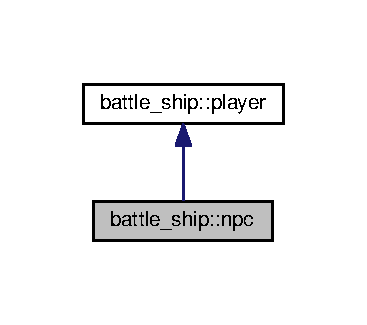
\includegraphics[width=176pt]{classbattle__ship_1_1npc__inherit__graph}
\end{center}
\end{figure}


Collaboration diagram for battle\+\_\+ship\+:\+:npc\+:
\nopagebreak
\begin{figure}[H]
\begin{center}
\leavevmode
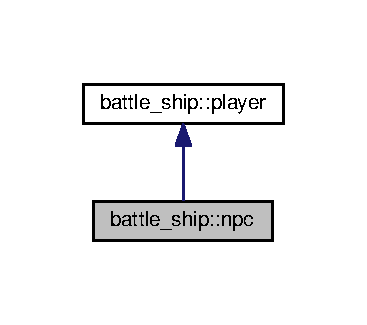
\includegraphics[width=176pt]{classbattle__ship_1_1npc__coll__graph}
\end{center}
\end{figure}
\subsection*{Public Member Functions}
\begin{DoxyCompactItemize}
\item 
\hyperlink{classbattle__ship_1_1npc_ab92a83aba6dbf1060ebdb666087790b8}{npc} ()=default
\item 
\hyperlink{classbattle__ship_1_1npc_a6a5c77aa108694177865edb9c2d06947}{npc} (std\+::string uname, size\+\_\+t diff)
\item 
void \hyperlink{classbattle__ship_1_1npc_a10c65edd38e75ac6be91ecd2dc9c9866}{winning\+\_\+line} ()
\begin{DoxyCompactList}\small\item\em Returns a line to be outputted when the user effectively loses. \end{DoxyCompactList}\item 
size\+\_\+t \hyperlink{classbattle__ship_1_1npc_acb3ad1c27c948ae968697c795f10a6b9}{get\+\_\+highscore} ()
\begin{DoxyCompactList}\small\item\em The N\+PC should not be saved in the all time highscores. \end{DoxyCompactList}\item 
void \hyperlink{classbattle__ship_1_1npc_ab81843d30e5f8801a8fe479d44ead157}{save\+\_\+highscore} (size\+\_\+t h)
\begin{DoxyCompactList}\small\item\em The N\+PC should not be saved in the all time highscores. \end{DoxyCompactList}\item 
void \hyperlink{classbattle__ship_1_1npc_abe6ec844c73c5410c2c4887fd50fac06}{attack} (\hyperlink{classbattle__ship_1_1piece}{piece} \&attacking\+\_\+piece, \hyperlink{classbattle__ship_1_1player}{player} \&\hyperlink{classbattle__ship_1_1player_af01292346caaf209039b6490ae18d8aa}{enemy})
\item 
\hyperlink{classbattle__ship_1_1npc_ab548776b810769c0af009f1db0df4ede}{$\sim$npc} ()=default
\end{DoxyCompactItemize}
\subsection*{Additional Inherited Members}


\subsection{Detailed Description}
A type of player, implements methods targeted for non-\/playable characters (computer controlled) 

\begin{DoxyAuthor}{Author}
Enrico Zammit Lonardelli
\end{DoxyAuthor}
Contact\+: \href{mailto:enrico.zammitl@gmail.com}{\tt enrico.\+zammitl@gmail.\+com}

Created on\+: Wed, 15 Apr 2020 17\+:55\+:28 

Definition at line 19 of file npc.\+h.



\subsection{Constructor \& Destructor Documentation}
\mbox{\Hypertarget{classbattle__ship_1_1npc_ab92a83aba6dbf1060ebdb666087790b8}\label{classbattle__ship_1_1npc_ab92a83aba6dbf1060ebdb666087790b8}} 
\index{battle\+\_\+ship\+::npc@{battle\+\_\+ship\+::npc}!npc@{npc}}
\index{npc@{npc}!battle\+\_\+ship\+::npc@{battle\+\_\+ship\+::npc}}
\subsubsection{\texorpdfstring{npc()}{npc()}\hspace{0.1cm}{\footnotesize\ttfamily [1/2]}}
{\footnotesize\ttfamily battle\+\_\+ship\+::npc\+::npc (\begin{DoxyParamCaption}{ }\end{DoxyParamCaption})\hspace{0.3cm}{\ttfamily [default]}}

\mbox{\Hypertarget{classbattle__ship_1_1npc_a6a5c77aa108694177865edb9c2d06947}\label{classbattle__ship_1_1npc_a6a5c77aa108694177865edb9c2d06947}} 
\index{battle\+\_\+ship\+::npc@{battle\+\_\+ship\+::npc}!npc@{npc}}
\index{npc@{npc}!battle\+\_\+ship\+::npc@{battle\+\_\+ship\+::npc}}
\subsubsection{\texorpdfstring{npc()}{npc()}\hspace{0.1cm}{\footnotesize\ttfamily [2/2]}}
{\footnotesize\ttfamily battle\+\_\+ship\+::npc\+::npc (\begin{DoxyParamCaption}\item[{std\+::string}]{uname,  }\item[{size\+\_\+t}]{diff }\end{DoxyParamCaption})\hspace{0.3cm}{\ttfamily [inline]}}



Definition at line 26 of file npc.\+h.

\mbox{\Hypertarget{classbattle__ship_1_1npc_ab548776b810769c0af009f1db0df4ede}\label{classbattle__ship_1_1npc_ab548776b810769c0af009f1db0df4ede}} 
\index{battle\+\_\+ship\+::npc@{battle\+\_\+ship\+::npc}!````~npc@{$\sim$npc}}
\index{````~npc@{$\sim$npc}!battle\+\_\+ship\+::npc@{battle\+\_\+ship\+::npc}}
\subsubsection{\texorpdfstring{$\sim$npc()}{~npc()}}
{\footnotesize\ttfamily battle\+\_\+ship\+::npc\+::$\sim$npc (\begin{DoxyParamCaption}{ }\end{DoxyParamCaption})\hspace{0.3cm}{\ttfamily [default]}}



\subsection{Member Function Documentation}
\mbox{\Hypertarget{classbattle__ship_1_1npc_abe6ec844c73c5410c2c4887fd50fac06}\label{classbattle__ship_1_1npc_abe6ec844c73c5410c2c4887fd50fac06}} 
\index{battle\+\_\+ship\+::npc@{battle\+\_\+ship\+::npc}!attack@{attack}}
\index{attack@{attack}!battle\+\_\+ship\+::npc@{battle\+\_\+ship\+::npc}}
\subsubsection{\texorpdfstring{attack()}{attack()}}
{\footnotesize\ttfamily void battle\+\_\+ship\+::npc\+::attack (\begin{DoxyParamCaption}\item[{\hyperlink{classbattle__ship_1_1piece}{battle\+\_\+ship\+::piece} \&}]{attacking\+\_\+piece,  }\item[{\hyperlink{classbattle__ship_1_1player}{battle\+\_\+ship\+::player} \&}]{enemy }\end{DoxyParamCaption})\hspace{0.3cm}{\ttfamily [virtual]}}



Implements \hyperlink{classbattle__ship_1_1player_a86be2256620cd5e20da6db7be8afdbc8}{battle\+\_\+ship\+::player}.



Definition at line 15 of file npc.\+cpp.

\mbox{\Hypertarget{classbattle__ship_1_1npc_acb3ad1c27c948ae968697c795f10a6b9}\label{classbattle__ship_1_1npc_acb3ad1c27c948ae968697c795f10a6b9}} 
\index{battle\+\_\+ship\+::npc@{battle\+\_\+ship\+::npc}!get\+\_\+highscore@{get\+\_\+highscore}}
\index{get\+\_\+highscore@{get\+\_\+highscore}!battle\+\_\+ship\+::npc@{battle\+\_\+ship\+::npc}}
\subsubsection{\texorpdfstring{get\+\_\+highscore()}{get\_highscore()}}
{\footnotesize\ttfamily size\+\_\+t battle\+\_\+ship\+::npc\+::get\+\_\+highscore (\begin{DoxyParamCaption}{ }\end{DoxyParamCaption})\hspace{0.3cm}{\ttfamily [inline]}, {\ttfamily [virtual]}}



The N\+PC should not be saved in the all time highscores. 



Implements \hyperlink{classbattle__ship_1_1player_a9b74e59f4b120d38ad591dba6a1d1ba7}{battle\+\_\+ship\+::player}.



Definition at line 31 of file npc.\+h.

\mbox{\Hypertarget{classbattle__ship_1_1npc_ab81843d30e5f8801a8fe479d44ead157}\label{classbattle__ship_1_1npc_ab81843d30e5f8801a8fe479d44ead157}} 
\index{battle\+\_\+ship\+::npc@{battle\+\_\+ship\+::npc}!save\+\_\+highscore@{save\+\_\+highscore}}
\index{save\+\_\+highscore@{save\+\_\+highscore}!battle\+\_\+ship\+::npc@{battle\+\_\+ship\+::npc}}
\subsubsection{\texorpdfstring{save\+\_\+highscore()}{save\_highscore()}}
{\footnotesize\ttfamily void battle\+\_\+ship\+::npc\+::save\+\_\+highscore (\begin{DoxyParamCaption}\item[{size\+\_\+t}]{h }\end{DoxyParamCaption})\hspace{0.3cm}{\ttfamily [inline]}, {\ttfamily [virtual]}}



The N\+PC should not be saved in the all time highscores. 



Implements \hyperlink{classbattle__ship_1_1player_a928538249678aea5402f8c673671e995}{battle\+\_\+ship\+::player}.



Definition at line 33 of file npc.\+h.

\mbox{\Hypertarget{classbattle__ship_1_1npc_a10c65edd38e75ac6be91ecd2dc9c9866}\label{classbattle__ship_1_1npc_a10c65edd38e75ac6be91ecd2dc9c9866}} 
\index{battle\+\_\+ship\+::npc@{battle\+\_\+ship\+::npc}!winning\+\_\+line@{winning\+\_\+line}}
\index{winning\+\_\+line@{winning\+\_\+line}!battle\+\_\+ship\+::npc@{battle\+\_\+ship\+::npc}}
\subsubsection{\texorpdfstring{winning\+\_\+line()}{winning\_line()}}
{\footnotesize\ttfamily void battle\+\_\+ship\+::npc\+::winning\+\_\+line (\begin{DoxyParamCaption}{ }\end{DoxyParamCaption})\hspace{0.3cm}{\ttfamily [virtual]}}



Returns a line to be outputted when the user effectively loses. 

The notifications are always addressing the user so npc winning is a negative message 

Implements \hyperlink{classbattle__ship_1_1player_a3110ec708fd8fc7e02a6e88a63d57d2f}{battle\+\_\+ship\+::player}.



Definition at line 11 of file npc.\+cpp.



The documentation for this class was generated from the following files\+:\begin{DoxyCompactItemize}
\item 
include/\hyperlink{npc_8h}{npc.\+h}\item 
src/\hyperlink{npc_8cpp}{npc.\+cpp}\end{DoxyCompactItemize}

\hypertarget{classbattle__ship_1_1piece}{}\section{battle\+\_\+ship\+:\+:piece Class Reference}
\label{classbattle__ship_1_1piece}\index{battle\+\_\+ship\+::piece@{battle\+\_\+ship\+::piece}}


{\ttfamily \#include $<$piece.\+h$>$}



Inheritance diagram for battle\+\_\+ship\+:\+:piece\+:
\nopagebreak
\begin{figure}[H]
\begin{center}
\leavevmode
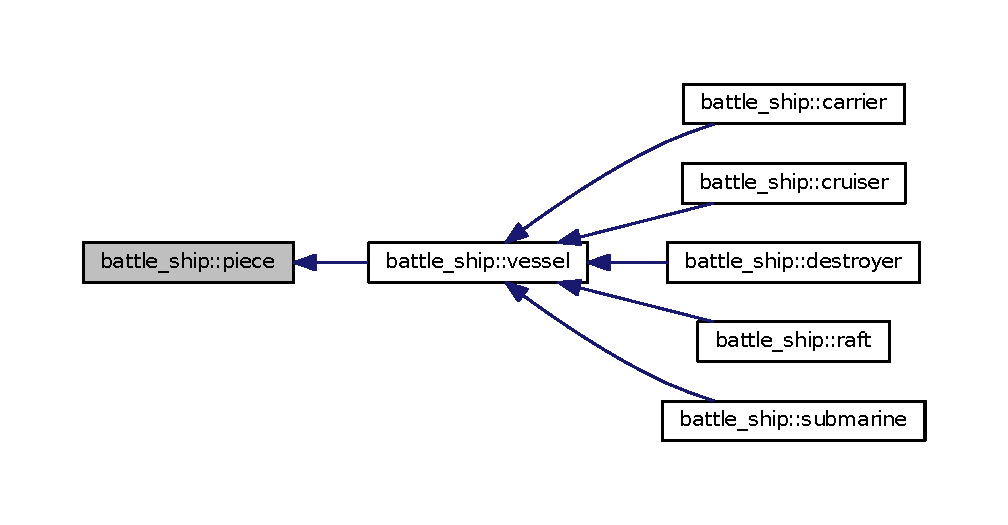
\includegraphics[width=350pt]{classbattle__ship_1_1piece__inherit__graph}
\end{center}
\end{figure}
\subsection*{Public Member Functions}
\begin{DoxyCompactItemize}
\item 
virtual std\+::vector$<$ std\+::string $>$ \hyperlink{classbattle__ship_1_1piece_aad848540970833ae5eadd115cc531b6b}{load\+\_\+image} () const =0
\item 
virtual \hyperlink{structbattle__ship_1_1coordinates}{coordinates} \hyperlink{classbattle__ship_1_1piece_a58092f7b1d663471204d7e51e68bbb2d}{calculate\+\_\+end} (\hyperlink{structbattle__ship_1_1coordinates}{coordinates} start, size\+\_\+t distance, \hyperlink{namespacebattle__ship_aed87488f0a73f0d0679fe343fb61c784}{orientation} o)=0
\item 
virtual void \hyperlink{classbattle__ship_1_1piece_a052305c855625732d3e5ba96d0fca5f9}{modify\+\_\+pose} (\hyperlink{structbattle__ship_1_1coordinates}{coordinates} new\+\_\+coors, \hyperlink{namespacebattle__ship_aed87488f0a73f0d0679fe343fb61c784}{orientation} new\+\_\+orientation)=0
\item 
virtual bool \hyperlink{classbattle__ship_1_1piece_af22bd781f4206decd0beed89b014d1cc}{has\+\_\+sunk} () const =0
\item 
virtual void \hyperlink{classbattle__ship_1_1piece_a77642906503e12eb22fcfbc3eab98cb5}{take\+\_\+hit} ()=0
\item 
virtual void \hyperlink{classbattle__ship_1_1piece_ad46ddc76d6e682a4f1fc8965a0c7813c}{display\+\_\+yz} ()=0
\item 
virtual void \hyperlink{classbattle__ship_1_1piece_a0f900b13641277ae9e809e4baa5c8c10}{display\+\_\+xy} ()=0
\item 
virtual std\+::size\+\_\+t \hyperlink{classbattle__ship_1_1piece_a08cfb1d99d1804f42f87878bef19e7ff}{get\+\_\+length} () const =0
\item 
virtual std\+::size\+\_\+t \hyperlink{classbattle__ship_1_1piece_a680897abc6ae9c5e187003a1c24fc9a1}{get\+\_\+width} () const =0
\item 
virtual std\+::string \hyperlink{classbattle__ship_1_1piece_aeba6c5083cb05200850cee7578a81d09}{get\+\_\+uri} () const =0
\item 
virtual std\+::size\+\_\+t \hyperlink{classbattle__ship_1_1piece_a27116e62c4ee91796349bbcb284e446d}{get\+\_\+hits} () const =0
\item 
virtual \hyperlink{namespacebattle__ship_aed87488f0a73f0d0679fe343fb61c784}{orientation} \hyperlink{classbattle__ship_1_1piece_a2cc01b1ec66bfb91df048401233e9618}{get\+\_\+orientation} () const =0
\item 
virtual std\+::string \hyperlink{classbattle__ship_1_1piece_ad589faff3ce07b5130bfdd89da4269c1}{get\+\_\+xy\+\_\+representation} () const =0
\item 
virtual std\+::string \hyperlink{classbattle__ship_1_1piece_a95531d660360ffc403a742db1b4f6413}{get\+\_\+name} () const =0
\item 
virtual int \hyperlink{classbattle__ship_1_1piece_a9193782bce8a697bd5d3cb391d5f1623}{get\+\_\+cost} () const =0
\item 
virtual \hyperlink{structbattle__ship_1_1coordinates}{coordinates} \hyperlink{classbattle__ship_1_1piece_ab5010cea30b96f5afc758b2a9d0d43bc}{get\+\_\+start} () const =0
\item 
virtual \hyperlink{structbattle__ship_1_1coordinates}{coordinates} \hyperlink{classbattle__ship_1_1piece_a4f7ac17a3ba66f104d2c5110e0fe51d4}{get\+\_\+end} () const =0
\item 
virtual size\+\_\+t \hyperlink{classbattle__ship_1_1piece_a63f00d666a65cd41a11b592d55411b7f}{get\+\_\+action\+\_\+points} ()=0
\end{DoxyCompactItemize}


\subsection{Detailed Description}


Definition at line 8 of file piece.\+h.



\subsection{Member Function Documentation}
\mbox{\Hypertarget{classbattle__ship_1_1piece_a58092f7b1d663471204d7e51e68bbb2d}\label{classbattle__ship_1_1piece_a58092f7b1d663471204d7e51e68bbb2d}} 
\index{battle\+\_\+ship\+::piece@{battle\+\_\+ship\+::piece}!calculate\+\_\+end@{calculate\+\_\+end}}
\index{calculate\+\_\+end@{calculate\+\_\+end}!battle\+\_\+ship\+::piece@{battle\+\_\+ship\+::piece}}
\subsubsection{\texorpdfstring{calculate\+\_\+end()}{calculate\_end()}}
{\footnotesize\ttfamily virtual \hyperlink{structbattle__ship_1_1coordinates}{coordinates} battle\+\_\+ship\+::piece\+::calculate\+\_\+end (\begin{DoxyParamCaption}\item[{\hyperlink{structbattle__ship_1_1coordinates}{coordinates}}]{start,  }\item[{size\+\_\+t}]{distance,  }\item[{\hyperlink{namespacebattle__ship_aed87488f0a73f0d0679fe343fb61c784}{orientation}}]{o }\end{DoxyParamCaption})\hspace{0.3cm}{\ttfamily [pure virtual]}}



Implemented in \hyperlink{classbattle__ship_1_1vessel_a9b99c5ed2629203985b25338df585234}{battle\+\_\+ship\+::vessel}.

\mbox{\Hypertarget{classbattle__ship_1_1piece_a0f900b13641277ae9e809e4baa5c8c10}\label{classbattle__ship_1_1piece_a0f900b13641277ae9e809e4baa5c8c10}} 
\index{battle\+\_\+ship\+::piece@{battle\+\_\+ship\+::piece}!display\+\_\+xy@{display\+\_\+xy}}
\index{display\+\_\+xy@{display\+\_\+xy}!battle\+\_\+ship\+::piece@{battle\+\_\+ship\+::piece}}
\subsubsection{\texorpdfstring{display\+\_\+xy()}{display\_xy()}}
{\footnotesize\ttfamily virtual void battle\+\_\+ship\+::piece\+::display\+\_\+xy (\begin{DoxyParamCaption}{ }\end{DoxyParamCaption})\hspace{0.3cm}{\ttfamily [pure virtual]}}



Implemented in \hyperlink{classbattle__ship_1_1vessel_a60924b058d686ebf545ae8f4d9f42d76}{battle\+\_\+ship\+::vessel}.

\mbox{\Hypertarget{classbattle__ship_1_1piece_ad46ddc76d6e682a4f1fc8965a0c7813c}\label{classbattle__ship_1_1piece_ad46ddc76d6e682a4f1fc8965a0c7813c}} 
\index{battle\+\_\+ship\+::piece@{battle\+\_\+ship\+::piece}!display\+\_\+yz@{display\+\_\+yz}}
\index{display\+\_\+yz@{display\+\_\+yz}!battle\+\_\+ship\+::piece@{battle\+\_\+ship\+::piece}}
\subsubsection{\texorpdfstring{display\+\_\+yz()}{display\_yz()}}
{\footnotesize\ttfamily virtual void battle\+\_\+ship\+::piece\+::display\+\_\+yz (\begin{DoxyParamCaption}{ }\end{DoxyParamCaption})\hspace{0.3cm}{\ttfamily [pure virtual]}}



Implemented in \hyperlink{classbattle__ship_1_1vessel_aa4f50939cb109b09c6b300313e193198}{battle\+\_\+ship\+::vessel}.

\mbox{\Hypertarget{classbattle__ship_1_1piece_a63f00d666a65cd41a11b592d55411b7f}\label{classbattle__ship_1_1piece_a63f00d666a65cd41a11b592d55411b7f}} 
\index{battle\+\_\+ship\+::piece@{battle\+\_\+ship\+::piece}!get\+\_\+action\+\_\+points@{get\+\_\+action\+\_\+points}}
\index{get\+\_\+action\+\_\+points@{get\+\_\+action\+\_\+points}!battle\+\_\+ship\+::piece@{battle\+\_\+ship\+::piece}}
\subsubsection{\texorpdfstring{get\+\_\+action\+\_\+points()}{get\_action\_points()}}
{\footnotesize\ttfamily virtual size\+\_\+t battle\+\_\+ship\+::piece\+::get\+\_\+action\+\_\+points (\begin{DoxyParamCaption}{ }\end{DoxyParamCaption})\hspace{0.3cm}{\ttfamily [pure virtual]}}



Implemented in \hyperlink{classbattle__ship_1_1vessel_a398b4134137d9e11c13e6aee548e1802}{battle\+\_\+ship\+::vessel}.

\mbox{\Hypertarget{classbattle__ship_1_1piece_a9193782bce8a697bd5d3cb391d5f1623}\label{classbattle__ship_1_1piece_a9193782bce8a697bd5d3cb391d5f1623}} 
\index{battle\+\_\+ship\+::piece@{battle\+\_\+ship\+::piece}!get\+\_\+cost@{get\+\_\+cost}}
\index{get\+\_\+cost@{get\+\_\+cost}!battle\+\_\+ship\+::piece@{battle\+\_\+ship\+::piece}}
\subsubsection{\texorpdfstring{get\+\_\+cost()}{get\_cost()}}
{\footnotesize\ttfamily virtual int battle\+\_\+ship\+::piece\+::get\+\_\+cost (\begin{DoxyParamCaption}{ }\end{DoxyParamCaption}) const\hspace{0.3cm}{\ttfamily [pure virtual]}}



Implemented in \hyperlink{classbattle__ship_1_1vessel_aadca1fe2ac265ed9f22e68490b6b22eb}{battle\+\_\+ship\+::vessel}.

\mbox{\Hypertarget{classbattle__ship_1_1piece_a4f7ac17a3ba66f104d2c5110e0fe51d4}\label{classbattle__ship_1_1piece_a4f7ac17a3ba66f104d2c5110e0fe51d4}} 
\index{battle\+\_\+ship\+::piece@{battle\+\_\+ship\+::piece}!get\+\_\+end@{get\+\_\+end}}
\index{get\+\_\+end@{get\+\_\+end}!battle\+\_\+ship\+::piece@{battle\+\_\+ship\+::piece}}
\subsubsection{\texorpdfstring{get\+\_\+end()}{get\_end()}}
{\footnotesize\ttfamily virtual \hyperlink{structbattle__ship_1_1coordinates}{coordinates} battle\+\_\+ship\+::piece\+::get\+\_\+end (\begin{DoxyParamCaption}{ }\end{DoxyParamCaption}) const\hspace{0.3cm}{\ttfamily [pure virtual]}}



Implemented in \hyperlink{classbattle__ship_1_1vessel_ab24ee1fe21632b510833c8369ef3560a}{battle\+\_\+ship\+::vessel}.

\mbox{\Hypertarget{classbattle__ship_1_1piece_a27116e62c4ee91796349bbcb284e446d}\label{classbattle__ship_1_1piece_a27116e62c4ee91796349bbcb284e446d}} 
\index{battle\+\_\+ship\+::piece@{battle\+\_\+ship\+::piece}!get\+\_\+hits@{get\+\_\+hits}}
\index{get\+\_\+hits@{get\+\_\+hits}!battle\+\_\+ship\+::piece@{battle\+\_\+ship\+::piece}}
\subsubsection{\texorpdfstring{get\+\_\+hits()}{get\_hits()}}
{\footnotesize\ttfamily virtual std\+::size\+\_\+t battle\+\_\+ship\+::piece\+::get\+\_\+hits (\begin{DoxyParamCaption}{ }\end{DoxyParamCaption}) const\hspace{0.3cm}{\ttfamily [pure virtual]}}



Implemented in \hyperlink{classbattle__ship_1_1vessel_a1d7fb8fe8e4454850c1cd7dbb4c70d49}{battle\+\_\+ship\+::vessel}.

\mbox{\Hypertarget{classbattle__ship_1_1piece_a08cfb1d99d1804f42f87878bef19e7ff}\label{classbattle__ship_1_1piece_a08cfb1d99d1804f42f87878bef19e7ff}} 
\index{battle\+\_\+ship\+::piece@{battle\+\_\+ship\+::piece}!get\+\_\+length@{get\+\_\+length}}
\index{get\+\_\+length@{get\+\_\+length}!battle\+\_\+ship\+::piece@{battle\+\_\+ship\+::piece}}
\subsubsection{\texorpdfstring{get\+\_\+length()}{get\_length()}}
{\footnotesize\ttfamily virtual std\+::size\+\_\+t battle\+\_\+ship\+::piece\+::get\+\_\+length (\begin{DoxyParamCaption}{ }\end{DoxyParamCaption}) const\hspace{0.3cm}{\ttfamily [pure virtual]}}



Implemented in \hyperlink{classbattle__ship_1_1vessel_a96d84d8ad107db77ae601d4e29471dde}{battle\+\_\+ship\+::vessel}.

\mbox{\Hypertarget{classbattle__ship_1_1piece_a95531d660360ffc403a742db1b4f6413}\label{classbattle__ship_1_1piece_a95531d660360ffc403a742db1b4f6413}} 
\index{battle\+\_\+ship\+::piece@{battle\+\_\+ship\+::piece}!get\+\_\+name@{get\+\_\+name}}
\index{get\+\_\+name@{get\+\_\+name}!battle\+\_\+ship\+::piece@{battle\+\_\+ship\+::piece}}
\subsubsection{\texorpdfstring{get\+\_\+name()}{get\_name()}}
{\footnotesize\ttfamily virtual std\+::string battle\+\_\+ship\+::piece\+::get\+\_\+name (\begin{DoxyParamCaption}{ }\end{DoxyParamCaption}) const\hspace{0.3cm}{\ttfamily [pure virtual]}}



Implemented in \hyperlink{classbattle__ship_1_1vessel_a623a1b35355db117b5381a3a0f5774eb}{battle\+\_\+ship\+::vessel}.

\mbox{\Hypertarget{classbattle__ship_1_1piece_a2cc01b1ec66bfb91df048401233e9618}\label{classbattle__ship_1_1piece_a2cc01b1ec66bfb91df048401233e9618}} 
\index{battle\+\_\+ship\+::piece@{battle\+\_\+ship\+::piece}!get\+\_\+orientation@{get\+\_\+orientation}}
\index{get\+\_\+orientation@{get\+\_\+orientation}!battle\+\_\+ship\+::piece@{battle\+\_\+ship\+::piece}}
\subsubsection{\texorpdfstring{get\+\_\+orientation()}{get\_orientation()}}
{\footnotesize\ttfamily virtual \hyperlink{namespacebattle__ship_aed87488f0a73f0d0679fe343fb61c784}{orientation} battle\+\_\+ship\+::piece\+::get\+\_\+orientation (\begin{DoxyParamCaption}{ }\end{DoxyParamCaption}) const\hspace{0.3cm}{\ttfamily [pure virtual]}}



Implemented in \hyperlink{classbattle__ship_1_1vessel_a698c7811878e56b7ba7eb6d88e6ac13f}{battle\+\_\+ship\+::vessel}.

\mbox{\Hypertarget{classbattle__ship_1_1piece_ab5010cea30b96f5afc758b2a9d0d43bc}\label{classbattle__ship_1_1piece_ab5010cea30b96f5afc758b2a9d0d43bc}} 
\index{battle\+\_\+ship\+::piece@{battle\+\_\+ship\+::piece}!get\+\_\+start@{get\+\_\+start}}
\index{get\+\_\+start@{get\+\_\+start}!battle\+\_\+ship\+::piece@{battle\+\_\+ship\+::piece}}
\subsubsection{\texorpdfstring{get\+\_\+start()}{get\_start()}}
{\footnotesize\ttfamily virtual \hyperlink{structbattle__ship_1_1coordinates}{coordinates} battle\+\_\+ship\+::piece\+::get\+\_\+start (\begin{DoxyParamCaption}{ }\end{DoxyParamCaption}) const\hspace{0.3cm}{\ttfamily [pure virtual]}}



Implemented in \hyperlink{classbattle__ship_1_1vessel_aba133e1debe50caa9cbbae5e867b5995}{battle\+\_\+ship\+::vessel}.

\mbox{\Hypertarget{classbattle__ship_1_1piece_aeba6c5083cb05200850cee7578a81d09}\label{classbattle__ship_1_1piece_aeba6c5083cb05200850cee7578a81d09}} 
\index{battle\+\_\+ship\+::piece@{battle\+\_\+ship\+::piece}!get\+\_\+uri@{get\+\_\+uri}}
\index{get\+\_\+uri@{get\+\_\+uri}!battle\+\_\+ship\+::piece@{battle\+\_\+ship\+::piece}}
\subsubsection{\texorpdfstring{get\+\_\+uri()}{get\_uri()}}
{\footnotesize\ttfamily virtual std\+::string battle\+\_\+ship\+::piece\+::get\+\_\+uri (\begin{DoxyParamCaption}{ }\end{DoxyParamCaption}) const\hspace{0.3cm}{\ttfamily [pure virtual]}}



Implemented in \hyperlink{classbattle__ship_1_1vessel_a3ab0850a3ccedf7e6083c7b494284289}{battle\+\_\+ship\+::vessel}.

\mbox{\Hypertarget{classbattle__ship_1_1piece_a680897abc6ae9c5e187003a1c24fc9a1}\label{classbattle__ship_1_1piece_a680897abc6ae9c5e187003a1c24fc9a1}} 
\index{battle\+\_\+ship\+::piece@{battle\+\_\+ship\+::piece}!get\+\_\+width@{get\+\_\+width}}
\index{get\+\_\+width@{get\+\_\+width}!battle\+\_\+ship\+::piece@{battle\+\_\+ship\+::piece}}
\subsubsection{\texorpdfstring{get\+\_\+width()}{get\_width()}}
{\footnotesize\ttfamily virtual std\+::size\+\_\+t battle\+\_\+ship\+::piece\+::get\+\_\+width (\begin{DoxyParamCaption}{ }\end{DoxyParamCaption}) const\hspace{0.3cm}{\ttfamily [pure virtual]}}



Implemented in \hyperlink{classbattle__ship_1_1vessel_a625d8f457a7afdafea7422ad89648123}{battle\+\_\+ship\+::vessel}.

\mbox{\Hypertarget{classbattle__ship_1_1piece_ad589faff3ce07b5130bfdd89da4269c1}\label{classbattle__ship_1_1piece_ad589faff3ce07b5130bfdd89da4269c1}} 
\index{battle\+\_\+ship\+::piece@{battle\+\_\+ship\+::piece}!get\+\_\+xy\+\_\+representation@{get\+\_\+xy\+\_\+representation}}
\index{get\+\_\+xy\+\_\+representation@{get\+\_\+xy\+\_\+representation}!battle\+\_\+ship\+::piece@{battle\+\_\+ship\+::piece}}
\subsubsection{\texorpdfstring{get\+\_\+xy\+\_\+representation()}{get\_xy\_representation()}}
{\footnotesize\ttfamily virtual std\+::string battle\+\_\+ship\+::piece\+::get\+\_\+xy\+\_\+representation (\begin{DoxyParamCaption}{ }\end{DoxyParamCaption}) const\hspace{0.3cm}{\ttfamily [pure virtual]}}



Implemented in \hyperlink{classbattle__ship_1_1vessel_a84bfaba9be4f15f6ec934c925d11967d}{battle\+\_\+ship\+::vessel}.

\mbox{\Hypertarget{classbattle__ship_1_1piece_af22bd781f4206decd0beed89b014d1cc}\label{classbattle__ship_1_1piece_af22bd781f4206decd0beed89b014d1cc}} 
\index{battle\+\_\+ship\+::piece@{battle\+\_\+ship\+::piece}!has\+\_\+sunk@{has\+\_\+sunk}}
\index{has\+\_\+sunk@{has\+\_\+sunk}!battle\+\_\+ship\+::piece@{battle\+\_\+ship\+::piece}}
\subsubsection{\texorpdfstring{has\+\_\+sunk()}{has\_sunk()}}
{\footnotesize\ttfamily virtual bool battle\+\_\+ship\+::piece\+::has\+\_\+sunk (\begin{DoxyParamCaption}{ }\end{DoxyParamCaption}) const\hspace{0.3cm}{\ttfamily [pure virtual]}}



Implemented in \hyperlink{classbattle__ship_1_1vessel_a5f36d687fbb87ced436d2d88847a1d5c}{battle\+\_\+ship\+::vessel}.

\mbox{\Hypertarget{classbattle__ship_1_1piece_aad848540970833ae5eadd115cc531b6b}\label{classbattle__ship_1_1piece_aad848540970833ae5eadd115cc531b6b}} 
\index{battle\+\_\+ship\+::piece@{battle\+\_\+ship\+::piece}!load\+\_\+image@{load\+\_\+image}}
\index{load\+\_\+image@{load\+\_\+image}!battle\+\_\+ship\+::piece@{battle\+\_\+ship\+::piece}}
\subsubsection{\texorpdfstring{load\+\_\+image()}{load\_image()}}
{\footnotesize\ttfamily virtual std\+::vector$<$std\+::string$>$ battle\+\_\+ship\+::piece\+::load\+\_\+image (\begin{DoxyParamCaption}{ }\end{DoxyParamCaption}) const\hspace{0.3cm}{\ttfamily [pure virtual]}}



Implemented in \hyperlink{classbattle__ship_1_1vessel_a36278b899be319a57cb728e8ecd2f340}{battle\+\_\+ship\+::vessel}.

\mbox{\Hypertarget{classbattle__ship_1_1piece_a052305c855625732d3e5ba96d0fca5f9}\label{classbattle__ship_1_1piece_a052305c855625732d3e5ba96d0fca5f9}} 
\index{battle\+\_\+ship\+::piece@{battle\+\_\+ship\+::piece}!modify\+\_\+pose@{modify\+\_\+pose}}
\index{modify\+\_\+pose@{modify\+\_\+pose}!battle\+\_\+ship\+::piece@{battle\+\_\+ship\+::piece}}
\subsubsection{\texorpdfstring{modify\+\_\+pose()}{modify\_pose()}}
{\footnotesize\ttfamily virtual void battle\+\_\+ship\+::piece\+::modify\+\_\+pose (\begin{DoxyParamCaption}\item[{\hyperlink{structbattle__ship_1_1coordinates}{coordinates}}]{new\+\_\+coors,  }\item[{\hyperlink{namespacebattle__ship_aed87488f0a73f0d0679fe343fb61c784}{orientation}}]{new\+\_\+orientation }\end{DoxyParamCaption})\hspace{0.3cm}{\ttfamily [pure virtual]}}



Implemented in \hyperlink{classbattle__ship_1_1vessel_ace0ec527147243b1fa6fa920d5a32a1f}{battle\+\_\+ship\+::vessel}.

\mbox{\Hypertarget{classbattle__ship_1_1piece_a77642906503e12eb22fcfbc3eab98cb5}\label{classbattle__ship_1_1piece_a77642906503e12eb22fcfbc3eab98cb5}} 
\index{battle\+\_\+ship\+::piece@{battle\+\_\+ship\+::piece}!take\+\_\+hit@{take\+\_\+hit}}
\index{take\+\_\+hit@{take\+\_\+hit}!battle\+\_\+ship\+::piece@{battle\+\_\+ship\+::piece}}
\subsubsection{\texorpdfstring{take\+\_\+hit()}{take\_hit()}}
{\footnotesize\ttfamily virtual void battle\+\_\+ship\+::piece\+::take\+\_\+hit (\begin{DoxyParamCaption}{ }\end{DoxyParamCaption})\hspace{0.3cm}{\ttfamily [pure virtual]}}



Implemented in \hyperlink{classbattle__ship_1_1vessel_ab0da3c305902d55594b7aa5d20b69509}{battle\+\_\+ship\+::vessel}.



The documentation for this class was generated from the following file\+:\begin{DoxyCompactItemize}
\item 
include/\hyperlink{piece_8h}{piece.\+h}\end{DoxyCompactItemize}

\hypertarget{classbattle__ship_1_1player}{}\section{battle\+\_\+ship\+:\+:player Class Reference}
\label{classbattle__ship_1_1player}\index{battle\+\_\+ship\+::player@{battle\+\_\+ship\+::player}}


{\ttfamily \#include $<$player.\+h$>$}



Inheritance diagram for battle\+\_\+ship\+:\+:player\+:
\nopagebreak
\begin{figure}[H]
\begin{center}
\leavevmode
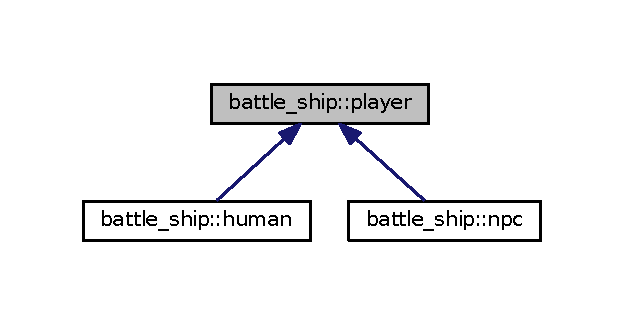
\includegraphics[width=300pt]{classbattle__ship_1_1player__inherit__graph}
\end{center}
\end{figure}
\subsection*{Public Member Functions}
\begin{DoxyCompactItemize}
\item 
\hyperlink{classbattle__ship_1_1player_a54df3c03653a24049b9629ce5c55fafa}{player} ()=default
\item 
\hyperlink{classbattle__ship_1_1player_a9c5da318ece63c6bdd3825cfa6ea9b4f}{player} (std\+::string uname, bool ready, std\+::string sub)
\item 
std\+::string \hyperlink{classbattle__ship_1_1player_a4a5406b436812664cb706c31b745239b}{get\+\_\+uname} ()
\item 
void \hyperlink{classbattle__ship_1_1player_a3525c2934ea6a4bd7600385cb5fa6bfa}{assign\+\_\+enemy} (std\+::shared\+\_\+ptr$<$ \hyperlink{classbattle__ship_1_1player}{player} $>$ e)
\item 
\hyperlink{classbattle__ship_1_1player}{player} \& \hyperlink{classbattle__ship_1_1player_a5224958feae654d622f56523dc45ab83}{get\+\_\+enemy} ()
\item 
void \hyperlink{classbattle__ship_1_1player_ade02279db7265558659c40f16c482df7}{modify\+\_\+budget} (int money)
\item 
void \hyperlink{classbattle__ship_1_1player_ae21fefa953f6a3a0476cabfae7084bbf}{reset} ()
\item 
bool \hyperlink{classbattle__ship_1_1player_af5373e08a637e9c21b3751eb02e07540}{is\+\_\+ready\+\_\+to\+\_\+play} ()
\item 
int \hyperlink{classbattle__ship_1_1player_ac2e25657d2330845c3770a75d107fef5}{get\+\_\+budget} ()
\item 
virtual void \hyperlink{classbattle__ship_1_1player_a3110ec708fd8fc7e02a6e88a63d57d2f}{winning\+\_\+line} ()=0
\item 
virtual void \hyperlink{classbattle__ship_1_1player_a86be2256620cd5e20da6db7be8afdbc8}{attack} (\hyperlink{classbattle__ship_1_1piece}{piece} \&attacking\+\_\+piece, \hyperlink{classbattle__ship_1_1player}{player} \&\hyperlink{classbattle__ship_1_1player_af01292346caaf209039b6490ae18d8aa}{enemy})=0
\item 
virtual size\+\_\+t \hyperlink{classbattle__ship_1_1player_a9b74e59f4b120d38ad591dba6a1d1ba7}{get\+\_\+highscore} ()=0
\item 
virtual void \hyperlink{classbattle__ship_1_1player_a928538249678aea5402f8c673671e995}{save\+\_\+highscore} (size\+\_\+t h)=0
\item 
\hyperlink{classbattle__ship_1_1board}{board} \& \hyperlink{classbattle__ship_1_1player_a57dacb55b2c506191d3d8426097c3c6a}{get\+\_\+board} ()
\item 
\hyperlink{classbattle__ship_1_1player_afbb6b6e880864bf7a36f21a95665a6c7}{$\sim$player} ()=default
\end{DoxyCompactItemize}
\subsection*{Protected Attributes}
\begin{DoxyCompactItemize}
\item 
std\+::string \hyperlink{classbattle__ship_1_1player_aed786567891bcafecb8610e12fb5d413}{username}
\item 
std\+::unique\+\_\+ptr$<$ \hyperlink{classbattle__ship_1_1board}{board} $>$ \hyperlink{classbattle__ship_1_1player_a7a463dddbc0cd8e9dfa3d2c41687e59e}{player\+\_\+board}
\item 
std\+::weak\+\_\+ptr$<$ \hyperlink{classbattle__ship_1_1player}{player} $>$ \hyperlink{classbattle__ship_1_1player_af01292346caaf209039b6490ae18d8aa}{enemy}
\item 
int \hyperlink{classbattle__ship_1_1player_a01f047aac5fcca92ff1e42d4d1e398c9}{budget} \{500\}
\item 
std\+::vector$<$ \hyperlink{structbattle__ship_1_1coordinates}{coordinates} $>$ \hyperlink{classbattle__ship_1_1player_ac0905b76a660cd06e5fd45f4960d48f9}{already\+\_\+targeted}
\item 
bool \hyperlink{classbattle__ship_1_1player_a48a3f8c692c7ea1def384c39b9b65e85}{ready\+\_\+to\+\_\+play}
\item 
std\+::string \hyperlink{classbattle__ship_1_1player_a5cb155ee3d722244c44bf71e5e2440c4}{subdir}
\end{DoxyCompactItemize}


\subsection{Detailed Description}


Definition at line 7 of file player.\+h.



\subsection{Constructor \& Destructor Documentation}
\mbox{\Hypertarget{classbattle__ship_1_1player_a54df3c03653a24049b9629ce5c55fafa}\label{classbattle__ship_1_1player_a54df3c03653a24049b9629ce5c55fafa}} 
\index{battle\+\_\+ship\+::player@{battle\+\_\+ship\+::player}!player@{player}}
\index{player@{player}!battle\+\_\+ship\+::player@{battle\+\_\+ship\+::player}}
\subsubsection{\texorpdfstring{player()}{player()}\hspace{0.1cm}{\footnotesize\ttfamily [1/2]}}
{\footnotesize\ttfamily battle\+\_\+ship\+::player\+::player (\begin{DoxyParamCaption}{ }\end{DoxyParamCaption})\hspace{0.3cm}{\ttfamily [default]}}

\mbox{\Hypertarget{classbattle__ship_1_1player_a9c5da318ece63c6bdd3825cfa6ea9b4f}\label{classbattle__ship_1_1player_a9c5da318ece63c6bdd3825cfa6ea9b4f}} 
\index{battle\+\_\+ship\+::player@{battle\+\_\+ship\+::player}!player@{player}}
\index{player@{player}!battle\+\_\+ship\+::player@{battle\+\_\+ship\+::player}}
\subsubsection{\texorpdfstring{player()}{player()}\hspace{0.1cm}{\footnotesize\ttfamily [2/2]}}
{\footnotesize\ttfamily battle\+\_\+ship\+::player\+::player (\begin{DoxyParamCaption}\item[{std\+::string}]{uname,  }\item[{bool}]{ready,  }\item[{std\+::string}]{sub }\end{DoxyParamCaption})\hspace{0.3cm}{\ttfamily [inline]}}



Definition at line 19 of file player.\+h.

\mbox{\Hypertarget{classbattle__ship_1_1player_afbb6b6e880864bf7a36f21a95665a6c7}\label{classbattle__ship_1_1player_afbb6b6e880864bf7a36f21a95665a6c7}} 
\index{battle\+\_\+ship\+::player@{battle\+\_\+ship\+::player}!````~player@{$\sim$player}}
\index{````~player@{$\sim$player}!battle\+\_\+ship\+::player@{battle\+\_\+ship\+::player}}
\subsubsection{\texorpdfstring{$\sim$player()}{~player()}}
{\footnotesize\ttfamily battle\+\_\+ship\+::player\+::$\sim$player (\begin{DoxyParamCaption}{ }\end{DoxyParamCaption})\hspace{0.3cm}{\ttfamily [default]}}



\subsection{Member Function Documentation}
\mbox{\Hypertarget{classbattle__ship_1_1player_a3525c2934ea6a4bd7600385cb5fa6bfa}\label{classbattle__ship_1_1player_a3525c2934ea6a4bd7600385cb5fa6bfa}} 
\index{battle\+\_\+ship\+::player@{battle\+\_\+ship\+::player}!assign\+\_\+enemy@{assign\+\_\+enemy}}
\index{assign\+\_\+enemy@{assign\+\_\+enemy}!battle\+\_\+ship\+::player@{battle\+\_\+ship\+::player}}
\subsubsection{\texorpdfstring{assign\+\_\+enemy()}{assign\_enemy()}}
{\footnotesize\ttfamily void battle\+\_\+ship\+::player\+::assign\+\_\+enemy (\begin{DoxyParamCaption}\item[{std\+::shared\+\_\+ptr$<$ \hyperlink{classbattle__ship_1_1player}{player} $>$}]{e }\end{DoxyParamCaption})\hspace{0.3cm}{\ttfamily [inline]}}



Definition at line 24 of file player.\+h.

\mbox{\Hypertarget{classbattle__ship_1_1player_a86be2256620cd5e20da6db7be8afdbc8}\label{classbattle__ship_1_1player_a86be2256620cd5e20da6db7be8afdbc8}} 
\index{battle\+\_\+ship\+::player@{battle\+\_\+ship\+::player}!attack@{attack}}
\index{attack@{attack}!battle\+\_\+ship\+::player@{battle\+\_\+ship\+::player}}
\subsubsection{\texorpdfstring{attack()}{attack()}}
{\footnotesize\ttfamily virtual void battle\+\_\+ship\+::player\+::attack (\begin{DoxyParamCaption}\item[{\hyperlink{classbattle__ship_1_1piece}{piece} \&}]{attacking\+\_\+piece,  }\item[{\hyperlink{classbattle__ship_1_1player}{player} \&}]{enemy }\end{DoxyParamCaption})\hspace{0.3cm}{\ttfamily [pure virtual]}}



Implemented in \hyperlink{classbattle__ship_1_1human_ad89701f0c4dd688c564b14a015059386}{battle\+\_\+ship\+::human}, and \hyperlink{classbattle__ship_1_1npc_abe6ec844c73c5410c2c4887fd50fac06}{battle\+\_\+ship\+::npc}.

\mbox{\Hypertarget{classbattle__ship_1_1player_a57dacb55b2c506191d3d8426097c3c6a}\label{classbattle__ship_1_1player_a57dacb55b2c506191d3d8426097c3c6a}} 
\index{battle\+\_\+ship\+::player@{battle\+\_\+ship\+::player}!get\+\_\+board@{get\+\_\+board}}
\index{get\+\_\+board@{get\+\_\+board}!battle\+\_\+ship\+::player@{battle\+\_\+ship\+::player}}
\subsubsection{\texorpdfstring{get\+\_\+board()}{get\_board()}}
{\footnotesize\ttfamily \hyperlink{classbattle__ship_1_1board}{board}\& battle\+\_\+ship\+::player\+::get\+\_\+board (\begin{DoxyParamCaption}{ }\end{DoxyParamCaption})\hspace{0.3cm}{\ttfamily [inline]}}



Definition at line 34 of file player.\+h.

\mbox{\Hypertarget{classbattle__ship_1_1player_ac2e25657d2330845c3770a75d107fef5}\label{classbattle__ship_1_1player_ac2e25657d2330845c3770a75d107fef5}} 
\index{battle\+\_\+ship\+::player@{battle\+\_\+ship\+::player}!get\+\_\+budget@{get\+\_\+budget}}
\index{get\+\_\+budget@{get\+\_\+budget}!battle\+\_\+ship\+::player@{battle\+\_\+ship\+::player}}
\subsubsection{\texorpdfstring{get\+\_\+budget()}{get\_budget()}}
{\footnotesize\ttfamily int battle\+\_\+ship\+::player\+::get\+\_\+budget (\begin{DoxyParamCaption}{ }\end{DoxyParamCaption})\hspace{0.3cm}{\ttfamily [inline]}}



Definition at line 29 of file player.\+h.

\mbox{\Hypertarget{classbattle__ship_1_1player_a5224958feae654d622f56523dc45ab83}\label{classbattle__ship_1_1player_a5224958feae654d622f56523dc45ab83}} 
\index{battle\+\_\+ship\+::player@{battle\+\_\+ship\+::player}!get\+\_\+enemy@{get\+\_\+enemy}}
\index{get\+\_\+enemy@{get\+\_\+enemy}!battle\+\_\+ship\+::player@{battle\+\_\+ship\+::player}}
\subsubsection{\texorpdfstring{get\+\_\+enemy()}{get\_enemy()}}
{\footnotesize\ttfamily \hyperlink{classbattle__ship_1_1player}{player}\& battle\+\_\+ship\+::player\+::get\+\_\+enemy (\begin{DoxyParamCaption}{ }\end{DoxyParamCaption})\hspace{0.3cm}{\ttfamily [inline]}}



Definition at line 25 of file player.\+h.

\mbox{\Hypertarget{classbattle__ship_1_1player_a9b74e59f4b120d38ad591dba6a1d1ba7}\label{classbattle__ship_1_1player_a9b74e59f4b120d38ad591dba6a1d1ba7}} 
\index{battle\+\_\+ship\+::player@{battle\+\_\+ship\+::player}!get\+\_\+highscore@{get\+\_\+highscore}}
\index{get\+\_\+highscore@{get\+\_\+highscore}!battle\+\_\+ship\+::player@{battle\+\_\+ship\+::player}}
\subsubsection{\texorpdfstring{get\+\_\+highscore()}{get\_highscore()}}
{\footnotesize\ttfamily virtual size\+\_\+t battle\+\_\+ship\+::player\+::get\+\_\+highscore (\begin{DoxyParamCaption}{ }\end{DoxyParamCaption})\hspace{0.3cm}{\ttfamily [pure virtual]}}



Implemented in \hyperlink{classbattle__ship_1_1npc_acb3ad1c27c948ae968697c795f10a6b9}{battle\+\_\+ship\+::npc}, and \hyperlink{classbattle__ship_1_1human_ac3529c252376938ce6b62ac40f8df3b3}{battle\+\_\+ship\+::human}.

\mbox{\Hypertarget{classbattle__ship_1_1player_a4a5406b436812664cb706c31b745239b}\label{classbattle__ship_1_1player_a4a5406b436812664cb706c31b745239b}} 
\index{battle\+\_\+ship\+::player@{battle\+\_\+ship\+::player}!get\+\_\+uname@{get\+\_\+uname}}
\index{get\+\_\+uname@{get\+\_\+uname}!battle\+\_\+ship\+::player@{battle\+\_\+ship\+::player}}
\subsubsection{\texorpdfstring{get\+\_\+uname()}{get\_uname()}}
{\footnotesize\ttfamily std\+::string battle\+\_\+ship\+::player\+::get\+\_\+uname (\begin{DoxyParamCaption}{ }\end{DoxyParamCaption})\hspace{0.3cm}{\ttfamily [inline]}}



Definition at line 23 of file player.\+h.

\mbox{\Hypertarget{classbattle__ship_1_1player_af5373e08a637e9c21b3751eb02e07540}\label{classbattle__ship_1_1player_af5373e08a637e9c21b3751eb02e07540}} 
\index{battle\+\_\+ship\+::player@{battle\+\_\+ship\+::player}!is\+\_\+ready\+\_\+to\+\_\+play@{is\+\_\+ready\+\_\+to\+\_\+play}}
\index{is\+\_\+ready\+\_\+to\+\_\+play@{is\+\_\+ready\+\_\+to\+\_\+play}!battle\+\_\+ship\+::player@{battle\+\_\+ship\+::player}}
\subsubsection{\texorpdfstring{is\+\_\+ready\+\_\+to\+\_\+play()}{is\_ready\_to\_play()}}
{\footnotesize\ttfamily bool battle\+\_\+ship\+::player\+::is\+\_\+ready\+\_\+to\+\_\+play (\begin{DoxyParamCaption}{ }\end{DoxyParamCaption})\hspace{0.3cm}{\ttfamily [inline]}}



Definition at line 28 of file player.\+h.

\mbox{\Hypertarget{classbattle__ship_1_1player_ade02279db7265558659c40f16c482df7}\label{classbattle__ship_1_1player_ade02279db7265558659c40f16c482df7}} 
\index{battle\+\_\+ship\+::player@{battle\+\_\+ship\+::player}!modify\+\_\+budget@{modify\+\_\+budget}}
\index{modify\+\_\+budget@{modify\+\_\+budget}!battle\+\_\+ship\+::player@{battle\+\_\+ship\+::player}}
\subsubsection{\texorpdfstring{modify\+\_\+budget()}{modify\_budget()}}
{\footnotesize\ttfamily void battle\+\_\+ship\+::player\+::modify\+\_\+budget (\begin{DoxyParamCaption}\item[{int}]{money }\end{DoxyParamCaption})\hspace{0.3cm}{\ttfamily [inline]}}



Definition at line 26 of file player.\+h.

\mbox{\Hypertarget{classbattle__ship_1_1player_ae21fefa953f6a3a0476cabfae7084bbf}\label{classbattle__ship_1_1player_ae21fefa953f6a3a0476cabfae7084bbf}} 
\index{battle\+\_\+ship\+::player@{battle\+\_\+ship\+::player}!reset@{reset}}
\index{reset@{reset}!battle\+\_\+ship\+::player@{battle\+\_\+ship\+::player}}
\subsubsection{\texorpdfstring{reset()}{reset()}}
{\footnotesize\ttfamily void battle\+\_\+ship\+::player\+::reset (\begin{DoxyParamCaption}{ }\end{DoxyParamCaption})}



Definition at line 7 of file player.\+cpp.

\mbox{\Hypertarget{classbattle__ship_1_1player_a928538249678aea5402f8c673671e995}\label{classbattle__ship_1_1player_a928538249678aea5402f8c673671e995}} 
\index{battle\+\_\+ship\+::player@{battle\+\_\+ship\+::player}!save\+\_\+highscore@{save\+\_\+highscore}}
\index{save\+\_\+highscore@{save\+\_\+highscore}!battle\+\_\+ship\+::player@{battle\+\_\+ship\+::player}}
\subsubsection{\texorpdfstring{save\+\_\+highscore()}{save\_highscore()}}
{\footnotesize\ttfamily virtual void battle\+\_\+ship\+::player\+::save\+\_\+highscore (\begin{DoxyParamCaption}\item[{size\+\_\+t}]{h }\end{DoxyParamCaption})\hspace{0.3cm}{\ttfamily [pure virtual]}}



Implemented in \hyperlink{classbattle__ship_1_1npc_ab81843d30e5f8801a8fe479d44ead157}{battle\+\_\+ship\+::npc}, and \hyperlink{classbattle__ship_1_1human_a5b7e6cad4d1f187907a205b767a2fd7d}{battle\+\_\+ship\+::human}.

\mbox{\Hypertarget{classbattle__ship_1_1player_a3110ec708fd8fc7e02a6e88a63d57d2f}\label{classbattle__ship_1_1player_a3110ec708fd8fc7e02a6e88a63d57d2f}} 
\index{battle\+\_\+ship\+::player@{battle\+\_\+ship\+::player}!winning\+\_\+line@{winning\+\_\+line}}
\index{winning\+\_\+line@{winning\+\_\+line}!battle\+\_\+ship\+::player@{battle\+\_\+ship\+::player}}
\subsubsection{\texorpdfstring{winning\+\_\+line()}{winning\_line()}}
{\footnotesize\ttfamily virtual void battle\+\_\+ship\+::player\+::winning\+\_\+line (\begin{DoxyParamCaption}{ }\end{DoxyParamCaption})\hspace{0.3cm}{\ttfamily [pure virtual]}}



Implemented in \hyperlink{classbattle__ship_1_1human_a583d0a9dd05c16f700d0d1825916faa3}{battle\+\_\+ship\+::human}, and \hyperlink{classbattle__ship_1_1npc_a10c65edd38e75ac6be91ecd2dc9c9866}{battle\+\_\+ship\+::npc}.



\subsection{Member Data Documentation}
\mbox{\Hypertarget{classbattle__ship_1_1player_ac0905b76a660cd06e5fd45f4960d48f9}\label{classbattle__ship_1_1player_ac0905b76a660cd06e5fd45f4960d48f9}} 
\index{battle\+\_\+ship\+::player@{battle\+\_\+ship\+::player}!already\+\_\+targeted@{already\+\_\+targeted}}
\index{already\+\_\+targeted@{already\+\_\+targeted}!battle\+\_\+ship\+::player@{battle\+\_\+ship\+::player}}
\subsubsection{\texorpdfstring{already\+\_\+targeted}{already\_targeted}}
{\footnotesize\ttfamily std\+::vector$<$\hyperlink{structbattle__ship_1_1coordinates}{coordinates}$>$ battle\+\_\+ship\+::player\+::already\+\_\+targeted\hspace{0.3cm}{\ttfamily [protected]}}



Definition at line 13 of file player.\+h.

\mbox{\Hypertarget{classbattle__ship_1_1player_a01f047aac5fcca92ff1e42d4d1e398c9}\label{classbattle__ship_1_1player_a01f047aac5fcca92ff1e42d4d1e398c9}} 
\index{battle\+\_\+ship\+::player@{battle\+\_\+ship\+::player}!budget@{budget}}
\index{budget@{budget}!battle\+\_\+ship\+::player@{battle\+\_\+ship\+::player}}
\subsubsection{\texorpdfstring{budget}{budget}}
{\footnotesize\ttfamily int battle\+\_\+ship\+::player\+::budget \{500\}\hspace{0.3cm}{\ttfamily [protected]}}



Definition at line 12 of file player.\+h.

\mbox{\Hypertarget{classbattle__ship_1_1player_af01292346caaf209039b6490ae18d8aa}\label{classbattle__ship_1_1player_af01292346caaf209039b6490ae18d8aa}} 
\index{battle\+\_\+ship\+::player@{battle\+\_\+ship\+::player}!enemy@{enemy}}
\index{enemy@{enemy}!battle\+\_\+ship\+::player@{battle\+\_\+ship\+::player}}
\subsubsection{\texorpdfstring{enemy}{enemy}}
{\footnotesize\ttfamily std\+::weak\+\_\+ptr$<$\hyperlink{classbattle__ship_1_1player}{player}$>$ battle\+\_\+ship\+::player\+::enemy\hspace{0.3cm}{\ttfamily [protected]}}



Definition at line 11 of file player.\+h.

\mbox{\Hypertarget{classbattle__ship_1_1player_a7a463dddbc0cd8e9dfa3d2c41687e59e}\label{classbattle__ship_1_1player_a7a463dddbc0cd8e9dfa3d2c41687e59e}} 
\index{battle\+\_\+ship\+::player@{battle\+\_\+ship\+::player}!player\+\_\+board@{player\+\_\+board}}
\index{player\+\_\+board@{player\+\_\+board}!battle\+\_\+ship\+::player@{battle\+\_\+ship\+::player}}
\subsubsection{\texorpdfstring{player\+\_\+board}{player\_board}}
{\footnotesize\ttfamily std\+::unique\+\_\+ptr$<$\hyperlink{classbattle__ship_1_1board}{board}$>$ battle\+\_\+ship\+::player\+::player\+\_\+board\hspace{0.3cm}{\ttfamily [protected]}}



Definition at line 10 of file player.\+h.

\mbox{\Hypertarget{classbattle__ship_1_1player_a48a3f8c692c7ea1def384c39b9b65e85}\label{classbattle__ship_1_1player_a48a3f8c692c7ea1def384c39b9b65e85}} 
\index{battle\+\_\+ship\+::player@{battle\+\_\+ship\+::player}!ready\+\_\+to\+\_\+play@{ready\+\_\+to\+\_\+play}}
\index{ready\+\_\+to\+\_\+play@{ready\+\_\+to\+\_\+play}!battle\+\_\+ship\+::player@{battle\+\_\+ship\+::player}}
\subsubsection{\texorpdfstring{ready\+\_\+to\+\_\+play}{ready\_to\_play}}
{\footnotesize\ttfamily bool battle\+\_\+ship\+::player\+::ready\+\_\+to\+\_\+play\hspace{0.3cm}{\ttfamily [protected]}}



Definition at line 14 of file player.\+h.

\mbox{\Hypertarget{classbattle__ship_1_1player_a5cb155ee3d722244c44bf71e5e2440c4}\label{classbattle__ship_1_1player_a5cb155ee3d722244c44bf71e5e2440c4}} 
\index{battle\+\_\+ship\+::player@{battle\+\_\+ship\+::player}!subdir@{subdir}}
\index{subdir@{subdir}!battle\+\_\+ship\+::player@{battle\+\_\+ship\+::player}}
\subsubsection{\texorpdfstring{subdir}{subdir}}
{\footnotesize\ttfamily std\+::string battle\+\_\+ship\+::player\+::subdir\hspace{0.3cm}{\ttfamily [protected]}}



Definition at line 15 of file player.\+h.

\mbox{\Hypertarget{classbattle__ship_1_1player_aed786567891bcafecb8610e12fb5d413}\label{classbattle__ship_1_1player_aed786567891bcafecb8610e12fb5d413}} 
\index{battle\+\_\+ship\+::player@{battle\+\_\+ship\+::player}!username@{username}}
\index{username@{username}!battle\+\_\+ship\+::player@{battle\+\_\+ship\+::player}}
\subsubsection{\texorpdfstring{username}{username}}
{\footnotesize\ttfamily std\+::string battle\+\_\+ship\+::player\+::username\hspace{0.3cm}{\ttfamily [protected]}}



Definition at line 9 of file player.\+h.



The documentation for this class was generated from the following files\+:\begin{DoxyCompactItemize}
\item 
include/\hyperlink{player_8h}{player.\+h}\item 
src/\hyperlink{player_8cpp}{player.\+cpp}\end{DoxyCompactItemize}

\hypertarget{classbattle__ship_1_1raft}{}\section{battle\+\_\+ship\+:\+:raft Class Reference}
\label{classbattle__ship_1_1raft}\index{battle\+\_\+ship\+::raft@{battle\+\_\+ship\+::raft}}


A type of vessel.  




{\ttfamily \#include $<$raft.\+h$>$}



Inheritance diagram for battle\+\_\+ship\+:\+:raft\+:
\nopagebreak
\begin{figure}[H]
\begin{center}
\leavevmode
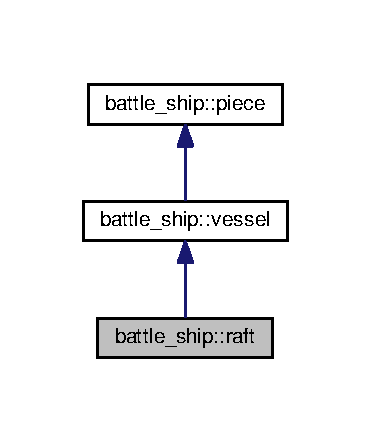
\includegraphics[width=178pt]{classbattle__ship_1_1raft__inherit__graph}
\end{center}
\end{figure}


Collaboration diagram for battle\+\_\+ship\+:\+:raft\+:
\nopagebreak
\begin{figure}[H]
\begin{center}
\leavevmode
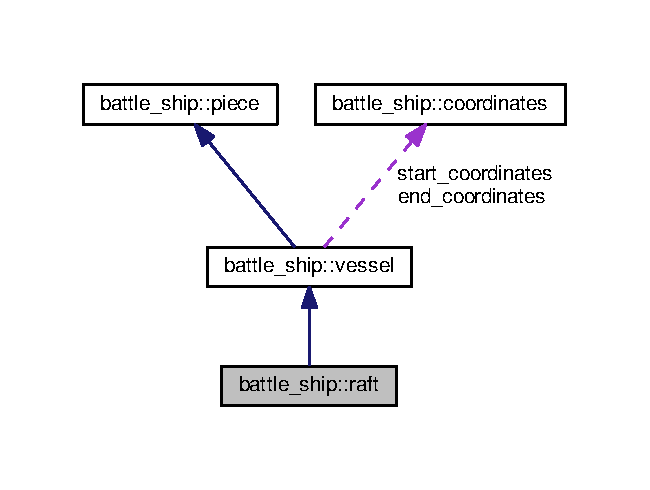
\includegraphics[width=312pt]{classbattle__ship_1_1raft__coll__graph}
\end{center}
\end{figure}
\subsection*{Public Member Functions}
\begin{DoxyCompactItemize}
\item 
\hyperlink{classbattle__ship_1_1raft_acde3f010cdf8cb639c6c9996c4a31656}{raft} ()=default
\item 
\hyperlink{classbattle__ship_1_1raft_ab76a787da1c470907eb7e166af6e0db8}{raft} (\hyperlink{structbattle__ship_1_1coordinates}{coordinates} p, \hyperlink{namespacebattle__ship_aed87488f0a73f0d0679fe343fb61c784}{orientation} o)
\item 
\hyperlink{classbattle__ship_1_1raft_a4b381ef568f95e3fe097eeef75d2ac51}{$\sim$raft} ()=default
\end{DoxyCompactItemize}
\subsection*{Additional Inherited Members}


\subsection{Detailed Description}
A type of vessel. 

\begin{DoxyAuthor}{Author}
Enrico Zammit Lonardelli
\end{DoxyAuthor}
Contact\+: \href{mailto:enrico.zammitl@gmail.com}{\tt enrico.\+zammitl@gmail.\+com}

Created on\+: Wed, 15 Apr 2020 21\+:32\+:31 

Definition at line 19 of file raft.\+h.



\subsection{Constructor \& Destructor Documentation}
\mbox{\Hypertarget{classbattle__ship_1_1raft_acde3f010cdf8cb639c6c9996c4a31656}\label{classbattle__ship_1_1raft_acde3f010cdf8cb639c6c9996c4a31656}} 
\index{battle\+\_\+ship\+::raft@{battle\+\_\+ship\+::raft}!raft@{raft}}
\index{raft@{raft}!battle\+\_\+ship\+::raft@{battle\+\_\+ship\+::raft}}
\subsubsection{\texorpdfstring{raft()}{raft()}\hspace{0.1cm}{\footnotesize\ttfamily [1/2]}}
{\footnotesize\ttfamily battle\+\_\+ship\+::raft\+::raft (\begin{DoxyParamCaption}{ }\end{DoxyParamCaption})\hspace{0.3cm}{\ttfamily [default]}}

\mbox{\Hypertarget{classbattle__ship_1_1raft_ab76a787da1c470907eb7e166af6e0db8}\label{classbattle__ship_1_1raft_ab76a787da1c470907eb7e166af6e0db8}} 
\index{battle\+\_\+ship\+::raft@{battle\+\_\+ship\+::raft}!raft@{raft}}
\index{raft@{raft}!battle\+\_\+ship\+::raft@{battle\+\_\+ship\+::raft}}
\subsubsection{\texorpdfstring{raft()}{raft()}\hspace{0.1cm}{\footnotesize\ttfamily [2/2]}}
{\footnotesize\ttfamily battle\+\_\+ship\+::raft\+::raft (\begin{DoxyParamCaption}\item[{\hyperlink{structbattle__ship_1_1coordinates}{coordinates}}]{p,  }\item[{\hyperlink{namespacebattle__ship_aed87488f0a73f0d0679fe343fb61c784}{orientation}}]{o }\end{DoxyParamCaption})\hspace{0.3cm}{\ttfamily [inline]}}



Definition at line 22 of file raft.\+h.

\mbox{\Hypertarget{classbattle__ship_1_1raft_a4b381ef568f95e3fe097eeef75d2ac51}\label{classbattle__ship_1_1raft_a4b381ef568f95e3fe097eeef75d2ac51}} 
\index{battle\+\_\+ship\+::raft@{battle\+\_\+ship\+::raft}!````~raft@{$\sim$raft}}
\index{````~raft@{$\sim$raft}!battle\+\_\+ship\+::raft@{battle\+\_\+ship\+::raft}}
\subsubsection{\texorpdfstring{$\sim$raft()}{~raft()}}
{\footnotesize\ttfamily battle\+\_\+ship\+::raft\+::$\sim$raft (\begin{DoxyParamCaption}{ }\end{DoxyParamCaption})\hspace{0.3cm}{\ttfamily [default]}}



The documentation for this class was generated from the following file\+:\begin{DoxyCompactItemize}
\item 
include/\hyperlink{raft_8h}{raft.\+h}\end{DoxyCompactItemize}

\hypertarget{classbattle__ship_1_1screen__manager}{}\section{battle\+\_\+ship\+:\+:screen\+\_\+manager Class Reference}
\label{classbattle__ship_1_1screen__manager}\index{battle\+\_\+ship\+::screen\+\_\+manager@{battle\+\_\+ship\+::screen\+\_\+manager}}


{\ttfamily \#include $<$screen\+\_\+manager.\+h$>$}

\subsection*{Static Public Member Functions}
\begin{DoxyCompactItemize}
\item 
static void \hyperlink{classbattle__ship_1_1screen__manager_a7463dbc1f9adcd2a2ee15d9874b01b01}{side\+\_\+by\+\_\+side} (\hyperlink{classbattle__ship_1_1game}{battle\+\_\+ship\+::game} \&\hyperlink{classbattle__ship_1_1game}{game}, std\+::size\+\_\+t width=5)
\end{DoxyCompactItemize}


\subsection{Detailed Description}


Definition at line 7 of file screen\+\_\+manager.\+h.



\subsection{Member Function Documentation}
\mbox{\Hypertarget{classbattle__ship_1_1screen__manager_a7463dbc1f9adcd2a2ee15d9874b01b01}\label{classbattle__ship_1_1screen__manager_a7463dbc1f9adcd2a2ee15d9874b01b01}} 
\index{battle\+\_\+ship\+::screen\+\_\+manager@{battle\+\_\+ship\+::screen\+\_\+manager}!side\+\_\+by\+\_\+side@{side\+\_\+by\+\_\+side}}
\index{side\+\_\+by\+\_\+side@{side\+\_\+by\+\_\+side}!battle\+\_\+ship\+::screen\+\_\+manager@{battle\+\_\+ship\+::screen\+\_\+manager}}
\subsubsection{\texorpdfstring{side\+\_\+by\+\_\+side()}{side\_by\_side()}}
{\footnotesize\ttfamily void battle\+\_\+ship\+::screen\+\_\+manager\+::side\+\_\+by\+\_\+side (\begin{DoxyParamCaption}\item[{\hyperlink{classbattle__ship_1_1game}{battle\+\_\+ship\+::game} \&}]{game,  }\item[{std\+::size\+\_\+t}]{width = {\ttfamily 5} }\end{DoxyParamCaption})\hspace{0.3cm}{\ttfamily [static]}}



Definition at line 9 of file screen\+\_\+manager.\+cpp.



The documentation for this class was generated from the following files\+:\begin{DoxyCompactItemize}
\item 
include/\hyperlink{screen__manager_8h}{screen\+\_\+manager.\+h}\item 
src/\hyperlink{screen__manager_8cpp}{screen\+\_\+manager.\+cpp}\end{DoxyCompactItemize}

\hypertarget{classbattle__ship_1_1submarine}{}\section{battle\+\_\+ship\+:\+:submarine Class Reference}
\label{classbattle__ship_1_1submarine}\index{battle\+\_\+ship\+::submarine@{battle\+\_\+ship\+::submarine}}


A type of vessel.  




{\ttfamily \#include $<$submarine.\+h$>$}



Inheritance diagram for battle\+\_\+ship\+:\+:submarine\+:
\nopagebreak
\begin{figure}[H]
\begin{center}
\leavevmode
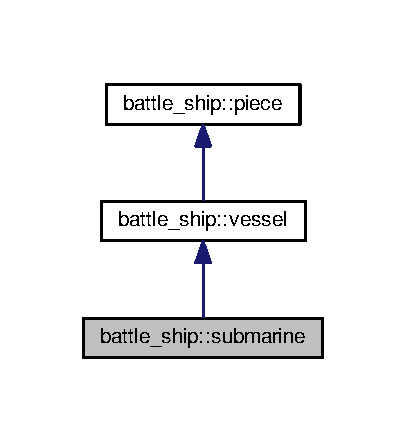
\includegraphics[width=195pt]{classbattle__ship_1_1submarine__inherit__graph}
\end{center}
\end{figure}


Collaboration diagram for battle\+\_\+ship\+:\+:submarine\+:
\nopagebreak
\begin{figure}[H]
\begin{center}
\leavevmode
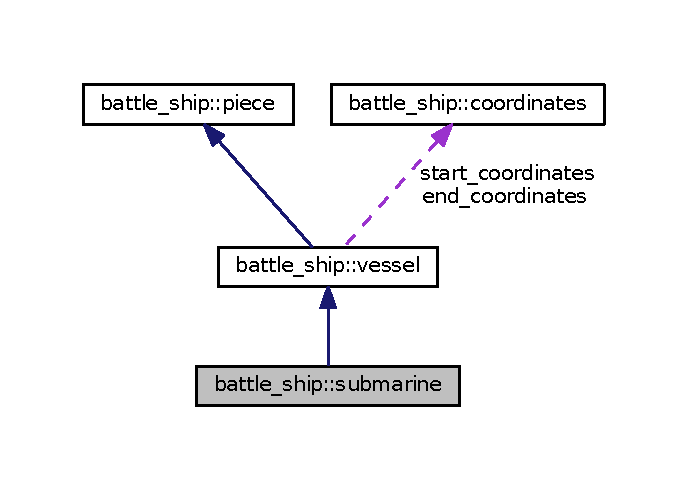
\includegraphics[width=312pt]{classbattle__ship_1_1submarine__coll__graph}
\end{center}
\end{figure}
\subsection*{Public Member Functions}
\begin{DoxyCompactItemize}
\item 
\hyperlink{classbattle__ship_1_1submarine_a52a8062290d2f36e162fc033a3917c5a}{submarine} ()=default
\item 
\hyperlink{classbattle__ship_1_1submarine_a229d0577e45bd964f4d32b50506c9504}{submarine} (\hyperlink{structbattle__ship_1_1coordinates}{coordinates} p, \hyperlink{namespacebattle__ship_aed87488f0a73f0d0679fe343fb61c784}{orientation} o)
\item 
\hyperlink{classbattle__ship_1_1submarine_a03b3a1b0c62de507e2b3a4d9ec1de06f}{$\sim$submarine} ()=default
\end{DoxyCompactItemize}
\subsection*{Additional Inherited Members}


\subsection{Detailed Description}
A type of vessel. 

\begin{DoxyAuthor}{Author}
Enrico Zammit Lonardelli
\end{DoxyAuthor}
Contact\+: \href{mailto:enrico.zammitl@gmail.com}{\tt enrico.\+zammitl@gmail.\+com}

Created on\+: Wed, 15 Apr 2020 21\+:32\+:31 

Definition at line 19 of file submarine.\+h.



\subsection{Constructor \& Destructor Documentation}
\mbox{\Hypertarget{classbattle__ship_1_1submarine_a52a8062290d2f36e162fc033a3917c5a}\label{classbattle__ship_1_1submarine_a52a8062290d2f36e162fc033a3917c5a}} 
\index{battle\+\_\+ship\+::submarine@{battle\+\_\+ship\+::submarine}!submarine@{submarine}}
\index{submarine@{submarine}!battle\+\_\+ship\+::submarine@{battle\+\_\+ship\+::submarine}}
\subsubsection{\texorpdfstring{submarine()}{submarine()}\hspace{0.1cm}{\footnotesize\ttfamily [1/2]}}
{\footnotesize\ttfamily battle\+\_\+ship\+::submarine\+::submarine (\begin{DoxyParamCaption}{ }\end{DoxyParamCaption})\hspace{0.3cm}{\ttfamily [default]}}

\mbox{\Hypertarget{classbattle__ship_1_1submarine_a229d0577e45bd964f4d32b50506c9504}\label{classbattle__ship_1_1submarine_a229d0577e45bd964f4d32b50506c9504}} 
\index{battle\+\_\+ship\+::submarine@{battle\+\_\+ship\+::submarine}!submarine@{submarine}}
\index{submarine@{submarine}!battle\+\_\+ship\+::submarine@{battle\+\_\+ship\+::submarine}}
\subsubsection{\texorpdfstring{submarine()}{submarine()}\hspace{0.1cm}{\footnotesize\ttfamily [2/2]}}
{\footnotesize\ttfamily battle\+\_\+ship\+::submarine\+::submarine (\begin{DoxyParamCaption}\item[{\hyperlink{structbattle__ship_1_1coordinates}{coordinates}}]{p,  }\item[{\hyperlink{namespacebattle__ship_aed87488f0a73f0d0679fe343fb61c784}{orientation}}]{o }\end{DoxyParamCaption})\hspace{0.3cm}{\ttfamily [inline]}}



Definition at line 22 of file submarine.\+h.

\mbox{\Hypertarget{classbattle__ship_1_1submarine_a03b3a1b0c62de507e2b3a4d9ec1de06f}\label{classbattle__ship_1_1submarine_a03b3a1b0c62de507e2b3a4d9ec1de06f}} 
\index{battle\+\_\+ship\+::submarine@{battle\+\_\+ship\+::submarine}!````~submarine@{$\sim$submarine}}
\index{````~submarine@{$\sim$submarine}!battle\+\_\+ship\+::submarine@{battle\+\_\+ship\+::submarine}}
\subsubsection{\texorpdfstring{$\sim$submarine()}{~submarine()}}
{\footnotesize\ttfamily battle\+\_\+ship\+::submarine\+::$\sim$submarine (\begin{DoxyParamCaption}{ }\end{DoxyParamCaption})\hspace{0.3cm}{\ttfamily [default]}}



The documentation for this class was generated from the following file\+:\begin{DoxyCompactItemize}
\item 
include/\hyperlink{submarine_8h}{submarine.\+h}\end{DoxyCompactItemize}

\hypertarget{classbattle__ship_1_1vessel}{}\section{battle\+\_\+ship\+:\+:vessel Class Reference}
\label{classbattle__ship_1_1vessel}\index{battle\+\_\+ship\+::vessel@{battle\+\_\+ship\+::vessel}}


Implements the methods for the abstract piece class.  




{\ttfamily \#include $<$vessel.\+h$>$}



Inheritance diagram for battle\+\_\+ship\+:\+:vessel\+:
\nopagebreak
\begin{figure}[H]
\begin{center}
\leavevmode
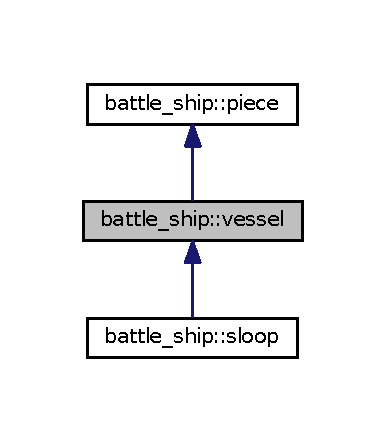
\includegraphics[width=350pt]{classbattle__ship_1_1vessel__inherit__graph}
\end{center}
\end{figure}


Collaboration diagram for battle\+\_\+ship\+:\+:vessel\+:
\nopagebreak
\begin{figure}[H]
\begin{center}
\leavevmode
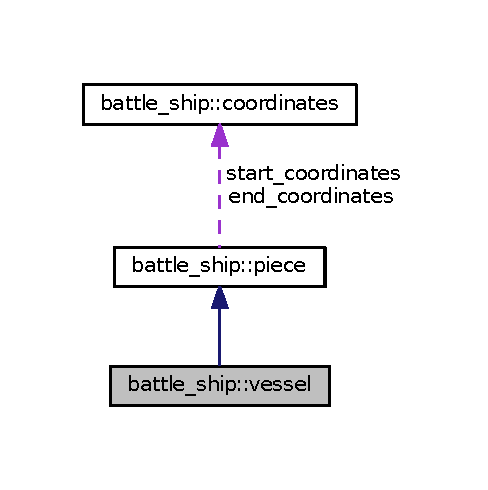
\includegraphics[width=312pt]{classbattle__ship_1_1vessel__coll__graph}
\end{center}
\end{figure}
\subsection*{Public Member Functions}
\begin{DoxyCompactItemize}
\item 
\hyperlink{classbattle__ship_1_1vessel_a6f3be9c2343940c262fb7add97402311}{vessel} ()=default
\item 
\hyperlink{classbattle__ship_1_1vessel_ade7f1d4ee4b458a715a0259e5211db20}{vessel} (std\+::string n, \hyperlink{structbattle__ship_1_1coordinates}{coordinates} p, size\+\_\+t l, size\+\_\+t w, std\+::string xy\+\_\+rep\+\_\+hor, std\+::string xy\+\_\+rep\+\_\+ver, \hyperlink{namespacebattle__ship_aed87488f0a73f0d0679fe343fb61c784}{orientation} o, size\+\_\+t ap)
\item 
\hyperlink{structbattle__ship_1_1coordinates}{coordinates} \hyperlink{classbattle__ship_1_1vessel_a9b99c5ed2629203985b25338df585234}{calculate\+\_\+end} (\hyperlink{structbattle__ship_1_1coordinates}{coordinates} start, size\+\_\+t distance, \hyperlink{namespacebattle__ship_aed87488f0a73f0d0679fe343fb61c784}{orientation} o) override
\begin{DoxyCompactList}\small\item\em Given a start coordinate calculate the end coordinate. \end{DoxyCompactList}\item 
void \hyperlink{classbattle__ship_1_1vessel_ace0ec527147243b1fa6fa920d5a32a1f}{modify\+\_\+pose} (\hyperlink{structbattle__ship_1_1coordinates}{coordinates} new\+\_\+coors, \hyperlink{namespacebattle__ship_aed87488f0a73f0d0679fe343fb61c784}{orientation} new\+\_\+orientation) override
\begin{DoxyCompactList}\small\item\em Modifies position and orientation. \end{DoxyCompactList}\item 
bool \hyperlink{classbattle__ship_1_1vessel_a5f36d687fbb87ced436d2d88847a1d5c}{has\+\_\+sunk} () const override
\item 
void \hyperlink{classbattle__ship_1_1vessel_ab0da3c305902d55594b7aa5d20b69509}{take\+\_\+hit} () override
\item 
void \hyperlink{classbattle__ship_1_1vessel_a60924b058d686ebf545ae8f4d9f42d76}{display\+\_\+xy} () override
\begin{DoxyCompactList}\small\item\em Displays what the top down view of this piece is. \end{DoxyCompactList}\item 
size\+\_\+t \hyperlink{classbattle__ship_1_1vessel_a398b4134137d9e11c13e6aee548e1802}{get\+\_\+action\+\_\+points} () override
\item 
size\+\_\+t \hyperlink{classbattle__ship_1_1vessel_ae166b521339b6a7b8c0be1a9d7861131}{get\+\_\+length} () const override
\item 
size\+\_\+t \hyperlink{classbattle__ship_1_1vessel_a84716baaafee9839292f67b03abc7272}{get\+\_\+width} () const override
\item 
size\+\_\+t \hyperlink{classbattle__ship_1_1vessel_a549dc0f3fc45f3b3f7fa247316900a9a}{get\+\_\+hits} () const override
\begin{DoxyCompactList}\small\item\em Returns the amount of hits already received from attacks. \end{DoxyCompactList}\item 
std\+::string \hyperlink{classbattle__ship_1_1vessel_a84bfaba9be4f15f6ec934c925d11967d}{get\+\_\+xy\+\_\+representation} () const override
\item 
\hyperlink{namespacebattle__ship_aed87488f0a73f0d0679fe343fb61c784}{orientation} \hyperlink{classbattle__ship_1_1vessel_a698c7811878e56b7ba7eb6d88e6ac13f}{get\+\_\+orientation} () const override
\item 
std\+::string \hyperlink{classbattle__ship_1_1vessel_a623a1b35355db117b5381a3a0f5774eb}{get\+\_\+name} () const override
\item 
\hyperlink{structbattle__ship_1_1coordinates}{coordinates} \hyperlink{classbattle__ship_1_1vessel_aba133e1debe50caa9cbbae5e867b5995}{get\+\_\+start} () const override
\item 
\hyperlink{structbattle__ship_1_1coordinates}{coordinates} \hyperlink{classbattle__ship_1_1vessel_ab24ee1fe21632b510833c8369ef3560a}{get\+\_\+end} () const override
\item 
int \hyperlink{classbattle__ship_1_1vessel_aadca1fe2ac265ed9f22e68490b6b22eb}{get\+\_\+cost} () const override
\item 
virtual \hyperlink{classbattle__ship_1_1vessel_a9e2c9554b6ce2af6f4e6168d1cf6591b}{$\sim$vessel} ()=default
\end{DoxyCompactItemize}
\subsection*{Protected Attributes}
\begin{DoxyCompactItemize}
\item 
std\+::string \hyperlink{classbattle__ship_1_1vessel_a7c7d199acda1b8914c1b014d7d2893b3}{name}
\item 
struct \hyperlink{structbattle__ship_1_1coordinates}{coordinates} \hyperlink{classbattle__ship_1_1vessel_a32625627454fc279169a7d94ef460cd4}{start\+\_\+coordinates}
\item 
struct \hyperlink{structbattle__ship_1_1coordinates}{coordinates} \hyperlink{classbattle__ship_1_1vessel_a90baf292572ee968095c107ec656db32}{end\+\_\+coordinates}
\item 
size\+\_\+t \hyperlink{classbattle__ship_1_1vessel_a51d62e0235c1c5b8116618a864d82929}{length}
\begin{DoxyCompactList}\small\item\em Defined as distance on the x-\/axis. \end{DoxyCompactList}\item 
size\+\_\+t \hyperlink{classbattle__ship_1_1vessel_ac69519345fd0c9a39b55a15516506461}{width}
\begin{DoxyCompactList}\small\item\em Defined as distance on the y-\/axis. \end{DoxyCompactList}\item 
std\+::string \hyperlink{classbattle__ship_1_1vessel_a563ede7bcd45c64f897f727ce2ca50ff}{xy\+\_\+representation\+\_\+horizontal}
\item 
std\+::string \hyperlink{classbattle__ship_1_1vessel_a7ab3092931ae7f230cb2cca77f2612c5}{xy\+\_\+representation\+\_\+vertical}
\item 
std\+::string \hyperlink{classbattle__ship_1_1vessel_ac49c1b9fd8b63846dac12053cebb1d00}{current\+\_\+xy\+\_\+representation}
\item 
\hyperlink{namespacebattle__ship_aed87488f0a73f0d0679fe343fb61c784}{orientation} \hyperlink{classbattle__ship_1_1vessel_ae0e05c0f43e6fe6c01bf1534ebece971}{current\+\_\+orientation}
\item 
int \hyperlink{classbattle__ship_1_1vessel_aaf2677260fd0f0ce56678cd23b8a0591}{cost} \{100\}
\item 
size\+\_\+t \hyperlink{classbattle__ship_1_1vessel_a1a14cc37d607ba7f3b710b36a11ff2e0}{hits} \{0\}
\item 
size\+\_\+t \hyperlink{classbattle__ship_1_1vessel_a5d2b710e2b58847818ba8e22794a97a4}{action\+\_\+points} \{0\}
\begin{DoxyCompactList}\small\item\em The number of turns this piece allows a player to attack if using it. \end{DoxyCompactList}\end{DoxyCompactItemize}


\subsection{Detailed Description}
Implements the methods for the abstract piece class. 

\begin{DoxyAuthor}{Author}
Enrico Zammit Lonardelli
\end{DoxyAuthor}
Contact\+: \href{mailto:enrico.zammitl@gmail.com}{\tt enrico.\+zammitl@gmail.\+com}

Created on\+: Sun, 29 Mar 2020 21\+:50\+:33 

Definition at line 21 of file vessel.\+h.



\subsection{Constructor \& Destructor Documentation}
\mbox{\Hypertarget{classbattle__ship_1_1vessel_a6f3be9c2343940c262fb7add97402311}\label{classbattle__ship_1_1vessel_a6f3be9c2343940c262fb7add97402311}} 
\index{battle\+\_\+ship\+::vessel@{battle\+\_\+ship\+::vessel}!vessel@{vessel}}
\index{vessel@{vessel}!battle\+\_\+ship\+::vessel@{battle\+\_\+ship\+::vessel}}
\subsubsection{\texorpdfstring{vessel()}{vessel()}\hspace{0.1cm}{\footnotesize\ttfamily [1/2]}}
{\footnotesize\ttfamily battle\+\_\+ship\+::vessel\+::vessel (\begin{DoxyParamCaption}{ }\end{DoxyParamCaption})\hspace{0.3cm}{\ttfamily [default]}}

\mbox{\Hypertarget{classbattle__ship_1_1vessel_ade7f1d4ee4b458a715a0259e5211db20}\label{classbattle__ship_1_1vessel_ade7f1d4ee4b458a715a0259e5211db20}} 
\index{battle\+\_\+ship\+::vessel@{battle\+\_\+ship\+::vessel}!vessel@{vessel}}
\index{vessel@{vessel}!battle\+\_\+ship\+::vessel@{battle\+\_\+ship\+::vessel}}
\subsubsection{\texorpdfstring{vessel()}{vessel()}\hspace{0.1cm}{\footnotesize\ttfamily [2/2]}}
{\footnotesize\ttfamily battle\+\_\+ship\+::vessel\+::vessel (\begin{DoxyParamCaption}\item[{std\+::string}]{n,  }\item[{\hyperlink{structbattle__ship_1_1coordinates}{battle\+\_\+ship\+::coordinates}}]{p,  }\item[{size\+\_\+t}]{l,  }\item[{size\+\_\+t}]{w,  }\item[{std\+::string}]{xy\+\_\+rep\+\_\+hor,  }\item[{std\+::string}]{xy\+\_\+rep\+\_\+ver,  }\item[{\hyperlink{namespacebattle__ship_aed87488f0a73f0d0679fe343fb61c784}{battle\+\_\+ship\+::orientation}}]{o,  }\item[{size\+\_\+t}]{ap }\end{DoxyParamCaption})}



Definition at line 9 of file vessel.\+cpp.

\mbox{\Hypertarget{classbattle__ship_1_1vessel_a9e2c9554b6ce2af6f4e6168d1cf6591b}\label{classbattle__ship_1_1vessel_a9e2c9554b6ce2af6f4e6168d1cf6591b}} 
\index{battle\+\_\+ship\+::vessel@{battle\+\_\+ship\+::vessel}!````~vessel@{$\sim$vessel}}
\index{````~vessel@{$\sim$vessel}!battle\+\_\+ship\+::vessel@{battle\+\_\+ship\+::vessel}}
\subsubsection{\texorpdfstring{$\sim$vessel()}{~vessel()}}
{\footnotesize\ttfamily virtual battle\+\_\+ship\+::vessel\+::$\sim$vessel (\begin{DoxyParamCaption}{ }\end{DoxyParamCaption})\hspace{0.3cm}{\ttfamily [virtual]}, {\ttfamily [default]}}



\subsection{Member Function Documentation}
\mbox{\Hypertarget{classbattle__ship_1_1vessel_a9b99c5ed2629203985b25338df585234}\label{classbattle__ship_1_1vessel_a9b99c5ed2629203985b25338df585234}} 
\index{battle\+\_\+ship\+::vessel@{battle\+\_\+ship\+::vessel}!calculate\+\_\+end@{calculate\+\_\+end}}
\index{calculate\+\_\+end@{calculate\+\_\+end}!battle\+\_\+ship\+::vessel@{battle\+\_\+ship\+::vessel}}
\subsubsection{\texorpdfstring{calculate\+\_\+end()}{calculate\_end()}}
{\footnotesize\ttfamily \hyperlink{structbattle__ship_1_1coordinates}{battle\+\_\+ship\+::coordinates} battle\+\_\+ship\+::vessel\+::calculate\+\_\+end (\begin{DoxyParamCaption}\item[{\hyperlink{structbattle__ship_1_1coordinates}{coordinates}}]{start,  }\item[{size\+\_\+t}]{distance,  }\item[{\hyperlink{namespacebattle__ship_aed87488f0a73f0d0679fe343fb61c784}{orientation}}]{o }\end{DoxyParamCaption})\hspace{0.3cm}{\ttfamily [override]}, {\ttfamily [virtual]}}



Given a start coordinate calculate the end coordinate. 



Implements \hyperlink{classbattle__ship_1_1piece_a58092f7b1d663471204d7e51e68bbb2d}{battle\+\_\+ship\+::piece}.



Definition at line 38 of file vessel.\+cpp.

\mbox{\Hypertarget{classbattle__ship_1_1vessel_a60924b058d686ebf545ae8f4d9f42d76}\label{classbattle__ship_1_1vessel_a60924b058d686ebf545ae8f4d9f42d76}} 
\index{battle\+\_\+ship\+::vessel@{battle\+\_\+ship\+::vessel}!display\+\_\+xy@{display\+\_\+xy}}
\index{display\+\_\+xy@{display\+\_\+xy}!battle\+\_\+ship\+::vessel@{battle\+\_\+ship\+::vessel}}
\subsubsection{\texorpdfstring{display\+\_\+xy()}{display\_xy()}}
{\footnotesize\ttfamily void battle\+\_\+ship\+::vessel\+::display\+\_\+xy (\begin{DoxyParamCaption}{ }\end{DoxyParamCaption})\hspace{0.3cm}{\ttfamily [override]}, {\ttfamily [virtual]}}



Displays what the top down view of this piece is. 



Implements \hyperlink{classbattle__ship_1_1piece_a0f900b13641277ae9e809e4baa5c8c10}{battle\+\_\+ship\+::piece}.



Definition at line 78 of file vessel.\+cpp.

\mbox{\Hypertarget{classbattle__ship_1_1vessel_a398b4134137d9e11c13e6aee548e1802}\label{classbattle__ship_1_1vessel_a398b4134137d9e11c13e6aee548e1802}} 
\index{battle\+\_\+ship\+::vessel@{battle\+\_\+ship\+::vessel}!get\+\_\+action\+\_\+points@{get\+\_\+action\+\_\+points}}
\index{get\+\_\+action\+\_\+points@{get\+\_\+action\+\_\+points}!battle\+\_\+ship\+::vessel@{battle\+\_\+ship\+::vessel}}
\subsubsection{\texorpdfstring{get\+\_\+action\+\_\+points()}{get\_action\_points()}}
{\footnotesize\ttfamily size\+\_\+t battle\+\_\+ship\+::vessel\+::get\+\_\+action\+\_\+points (\begin{DoxyParamCaption}{ }\end{DoxyParamCaption})\hspace{0.3cm}{\ttfamily [inline]}, {\ttfamily [override]}, {\ttfamily [virtual]}}



Implements \hyperlink{classbattle__ship_1_1piece_a63f00d666a65cd41a11b592d55411b7f}{battle\+\_\+ship\+::piece}.



Definition at line 50 of file vessel.\+h.

\mbox{\Hypertarget{classbattle__ship_1_1vessel_aadca1fe2ac265ed9f22e68490b6b22eb}\label{classbattle__ship_1_1vessel_aadca1fe2ac265ed9f22e68490b6b22eb}} 
\index{battle\+\_\+ship\+::vessel@{battle\+\_\+ship\+::vessel}!get\+\_\+cost@{get\+\_\+cost}}
\index{get\+\_\+cost@{get\+\_\+cost}!battle\+\_\+ship\+::vessel@{battle\+\_\+ship\+::vessel}}
\subsubsection{\texorpdfstring{get\+\_\+cost()}{get\_cost()}}
{\footnotesize\ttfamily int battle\+\_\+ship\+::vessel\+::get\+\_\+cost (\begin{DoxyParamCaption}{ }\end{DoxyParamCaption}) const\hspace{0.3cm}{\ttfamily [inline]}, {\ttfamily [override]}, {\ttfamily [virtual]}}



Implements \hyperlink{classbattle__ship_1_1piece_a9193782bce8a697bd5d3cb391d5f1623}{battle\+\_\+ship\+::piece}.



Definition at line 61 of file vessel.\+h.

\mbox{\Hypertarget{classbattle__ship_1_1vessel_ab24ee1fe21632b510833c8369ef3560a}\label{classbattle__ship_1_1vessel_ab24ee1fe21632b510833c8369ef3560a}} 
\index{battle\+\_\+ship\+::vessel@{battle\+\_\+ship\+::vessel}!get\+\_\+end@{get\+\_\+end}}
\index{get\+\_\+end@{get\+\_\+end}!battle\+\_\+ship\+::vessel@{battle\+\_\+ship\+::vessel}}
\subsubsection{\texorpdfstring{get\+\_\+end()}{get\_end()}}
{\footnotesize\ttfamily \hyperlink{structbattle__ship_1_1coordinates}{coordinates} battle\+\_\+ship\+::vessel\+::get\+\_\+end (\begin{DoxyParamCaption}{ }\end{DoxyParamCaption}) const\hspace{0.3cm}{\ttfamily [inline]}, {\ttfamily [override]}, {\ttfamily [virtual]}}



Implements \hyperlink{classbattle__ship_1_1piece_a4f7ac17a3ba66f104d2c5110e0fe51d4}{battle\+\_\+ship\+::piece}.



Definition at line 60 of file vessel.\+h.

\mbox{\Hypertarget{classbattle__ship_1_1vessel_a549dc0f3fc45f3b3f7fa247316900a9a}\label{classbattle__ship_1_1vessel_a549dc0f3fc45f3b3f7fa247316900a9a}} 
\index{battle\+\_\+ship\+::vessel@{battle\+\_\+ship\+::vessel}!get\+\_\+hits@{get\+\_\+hits}}
\index{get\+\_\+hits@{get\+\_\+hits}!battle\+\_\+ship\+::vessel@{battle\+\_\+ship\+::vessel}}
\subsubsection{\texorpdfstring{get\+\_\+hits()}{get\_hits()}}
{\footnotesize\ttfamily size\+\_\+t battle\+\_\+ship\+::vessel\+::get\+\_\+hits (\begin{DoxyParamCaption}{ }\end{DoxyParamCaption}) const\hspace{0.3cm}{\ttfamily [inline]}, {\ttfamily [override]}, {\ttfamily [virtual]}}



Returns the amount of hits already received from attacks. 



Implements \hyperlink{classbattle__ship_1_1piece_a51123474a964caa97a4c29b053ac0fad}{battle\+\_\+ship\+::piece}.



Definition at line 53 of file vessel.\+h.

\mbox{\Hypertarget{classbattle__ship_1_1vessel_ae166b521339b6a7b8c0be1a9d7861131}\label{classbattle__ship_1_1vessel_ae166b521339b6a7b8c0be1a9d7861131}} 
\index{battle\+\_\+ship\+::vessel@{battle\+\_\+ship\+::vessel}!get\+\_\+length@{get\+\_\+length}}
\index{get\+\_\+length@{get\+\_\+length}!battle\+\_\+ship\+::vessel@{battle\+\_\+ship\+::vessel}}
\subsubsection{\texorpdfstring{get\+\_\+length()}{get\_length()}}
{\footnotesize\ttfamily size\+\_\+t battle\+\_\+ship\+::vessel\+::get\+\_\+length (\begin{DoxyParamCaption}{ }\end{DoxyParamCaption}) const\hspace{0.3cm}{\ttfamily [inline]}, {\ttfamily [override]}, {\ttfamily [virtual]}}



Implements \hyperlink{classbattle__ship_1_1piece_a0188cda34ef90374396c52595761ef08}{battle\+\_\+ship\+::piece}.



Definition at line 51 of file vessel.\+h.

\mbox{\Hypertarget{classbattle__ship_1_1vessel_a623a1b35355db117b5381a3a0f5774eb}\label{classbattle__ship_1_1vessel_a623a1b35355db117b5381a3a0f5774eb}} 
\index{battle\+\_\+ship\+::vessel@{battle\+\_\+ship\+::vessel}!get\+\_\+name@{get\+\_\+name}}
\index{get\+\_\+name@{get\+\_\+name}!battle\+\_\+ship\+::vessel@{battle\+\_\+ship\+::vessel}}
\subsubsection{\texorpdfstring{get\+\_\+name()}{get\_name()}}
{\footnotesize\ttfamily std\+::string battle\+\_\+ship\+::vessel\+::get\+\_\+name (\begin{DoxyParamCaption}{ }\end{DoxyParamCaption}) const\hspace{0.3cm}{\ttfamily [inline]}, {\ttfamily [override]}, {\ttfamily [virtual]}}



Implements \hyperlink{classbattle__ship_1_1piece_a95531d660360ffc403a742db1b4f6413}{battle\+\_\+ship\+::piece}.



Definition at line 58 of file vessel.\+h.

\mbox{\Hypertarget{classbattle__ship_1_1vessel_a698c7811878e56b7ba7eb6d88e6ac13f}\label{classbattle__ship_1_1vessel_a698c7811878e56b7ba7eb6d88e6ac13f}} 
\index{battle\+\_\+ship\+::vessel@{battle\+\_\+ship\+::vessel}!get\+\_\+orientation@{get\+\_\+orientation}}
\index{get\+\_\+orientation@{get\+\_\+orientation}!battle\+\_\+ship\+::vessel@{battle\+\_\+ship\+::vessel}}
\subsubsection{\texorpdfstring{get\+\_\+orientation()}{get\_orientation()}}
{\footnotesize\ttfamily \hyperlink{namespacebattle__ship_aed87488f0a73f0d0679fe343fb61c784}{orientation} battle\+\_\+ship\+::vessel\+::get\+\_\+orientation (\begin{DoxyParamCaption}{ }\end{DoxyParamCaption}) const\hspace{0.3cm}{\ttfamily [inline]}, {\ttfamily [override]}, {\ttfamily [virtual]}}



Implements \hyperlink{classbattle__ship_1_1piece_a2cc01b1ec66bfb91df048401233e9618}{battle\+\_\+ship\+::piece}.



Definition at line 57 of file vessel.\+h.

\mbox{\Hypertarget{classbattle__ship_1_1vessel_aba133e1debe50caa9cbbae5e867b5995}\label{classbattle__ship_1_1vessel_aba133e1debe50caa9cbbae5e867b5995}} 
\index{battle\+\_\+ship\+::vessel@{battle\+\_\+ship\+::vessel}!get\+\_\+start@{get\+\_\+start}}
\index{get\+\_\+start@{get\+\_\+start}!battle\+\_\+ship\+::vessel@{battle\+\_\+ship\+::vessel}}
\subsubsection{\texorpdfstring{get\+\_\+start()}{get\_start()}}
{\footnotesize\ttfamily \hyperlink{structbattle__ship_1_1coordinates}{coordinates} battle\+\_\+ship\+::vessel\+::get\+\_\+start (\begin{DoxyParamCaption}{ }\end{DoxyParamCaption}) const\hspace{0.3cm}{\ttfamily [inline]}, {\ttfamily [override]}, {\ttfamily [virtual]}}



Implements \hyperlink{classbattle__ship_1_1piece_ab5010cea30b96f5afc758b2a9d0d43bc}{battle\+\_\+ship\+::piece}.



Definition at line 59 of file vessel.\+h.

\mbox{\Hypertarget{classbattle__ship_1_1vessel_a84716baaafee9839292f67b03abc7272}\label{classbattle__ship_1_1vessel_a84716baaafee9839292f67b03abc7272}} 
\index{battle\+\_\+ship\+::vessel@{battle\+\_\+ship\+::vessel}!get\+\_\+width@{get\+\_\+width}}
\index{get\+\_\+width@{get\+\_\+width}!battle\+\_\+ship\+::vessel@{battle\+\_\+ship\+::vessel}}
\subsubsection{\texorpdfstring{get\+\_\+width()}{get\_width()}}
{\footnotesize\ttfamily size\+\_\+t battle\+\_\+ship\+::vessel\+::get\+\_\+width (\begin{DoxyParamCaption}{ }\end{DoxyParamCaption}) const\hspace{0.3cm}{\ttfamily [inline]}, {\ttfamily [override]}, {\ttfamily [virtual]}}



Implements \hyperlink{classbattle__ship_1_1piece_abd5b9073f2fa6201c4dbc35b43942d2f}{battle\+\_\+ship\+::piece}.



Definition at line 52 of file vessel.\+h.

\mbox{\Hypertarget{classbattle__ship_1_1vessel_a84bfaba9be4f15f6ec934c925d11967d}\label{classbattle__ship_1_1vessel_a84bfaba9be4f15f6ec934c925d11967d}} 
\index{battle\+\_\+ship\+::vessel@{battle\+\_\+ship\+::vessel}!get\+\_\+xy\+\_\+representation@{get\+\_\+xy\+\_\+representation}}
\index{get\+\_\+xy\+\_\+representation@{get\+\_\+xy\+\_\+representation}!battle\+\_\+ship\+::vessel@{battle\+\_\+ship\+::vessel}}
\subsubsection{\texorpdfstring{get\+\_\+xy\+\_\+representation()}{get\_xy\_representation()}}
{\footnotesize\ttfamily std\+::string battle\+\_\+ship\+::vessel\+::get\+\_\+xy\+\_\+representation (\begin{DoxyParamCaption}{ }\end{DoxyParamCaption}) const\hspace{0.3cm}{\ttfamily [inline]}, {\ttfamily [override]}, {\ttfamily [virtual]}}



Implements \hyperlink{classbattle__ship_1_1piece_ad589faff3ce07b5130bfdd89da4269c1}{battle\+\_\+ship\+::piece}.



Definition at line 54 of file vessel.\+h.

\mbox{\Hypertarget{classbattle__ship_1_1vessel_a5f36d687fbb87ced436d2d88847a1d5c}\label{classbattle__ship_1_1vessel_a5f36d687fbb87ced436d2d88847a1d5c}} 
\index{battle\+\_\+ship\+::vessel@{battle\+\_\+ship\+::vessel}!has\+\_\+sunk@{has\+\_\+sunk}}
\index{has\+\_\+sunk@{has\+\_\+sunk}!battle\+\_\+ship\+::vessel@{battle\+\_\+ship\+::vessel}}
\subsubsection{\texorpdfstring{has\+\_\+sunk()}{has\_sunk()}}
{\footnotesize\ttfamily bool battle\+\_\+ship\+::vessel\+::has\+\_\+sunk (\begin{DoxyParamCaption}{ }\end{DoxyParamCaption}) const\hspace{0.3cm}{\ttfamily [inline]}, {\ttfamily [override]}, {\ttfamily [virtual]}}



Implements \hyperlink{classbattle__ship_1_1piece_af22bd781f4206decd0beed89b014d1cc}{battle\+\_\+ship\+::piece}.



Definition at line 47 of file vessel.\+h.

\mbox{\Hypertarget{classbattle__ship_1_1vessel_ace0ec527147243b1fa6fa920d5a32a1f}\label{classbattle__ship_1_1vessel_ace0ec527147243b1fa6fa920d5a32a1f}} 
\index{battle\+\_\+ship\+::vessel@{battle\+\_\+ship\+::vessel}!modify\+\_\+pose@{modify\+\_\+pose}}
\index{modify\+\_\+pose@{modify\+\_\+pose}!battle\+\_\+ship\+::vessel@{battle\+\_\+ship\+::vessel}}
\subsubsection{\texorpdfstring{modify\+\_\+pose()}{modify\_pose()}}
{\footnotesize\ttfamily void battle\+\_\+ship\+::vessel\+::modify\+\_\+pose (\begin{DoxyParamCaption}\item[{\hyperlink{structbattle__ship_1_1coordinates}{coordinates}}]{new\+\_\+coors,  }\item[{\hyperlink{namespacebattle__ship_aed87488f0a73f0d0679fe343fb61c784}{orientation}}]{new\+\_\+orientation }\end{DoxyParamCaption})\hspace{0.3cm}{\ttfamily [override]}, {\ttfamily [virtual]}}



Modifies position and orientation. 



Implements \hyperlink{classbattle__ship_1_1piece_a052305c855625732d3e5ba96d0fca5f9}{battle\+\_\+ship\+::piece}.



Definition at line 54 of file vessel.\+cpp.

\mbox{\Hypertarget{classbattle__ship_1_1vessel_ab0da3c305902d55594b7aa5d20b69509}\label{classbattle__ship_1_1vessel_ab0da3c305902d55594b7aa5d20b69509}} 
\index{battle\+\_\+ship\+::vessel@{battle\+\_\+ship\+::vessel}!take\+\_\+hit@{take\+\_\+hit}}
\index{take\+\_\+hit@{take\+\_\+hit}!battle\+\_\+ship\+::vessel@{battle\+\_\+ship\+::vessel}}
\subsubsection{\texorpdfstring{take\+\_\+hit()}{take\_hit()}}
{\footnotesize\ttfamily void battle\+\_\+ship\+::vessel\+::take\+\_\+hit (\begin{DoxyParamCaption}{ }\end{DoxyParamCaption})\hspace{0.3cm}{\ttfamily [inline]}, {\ttfamily [override]}, {\ttfamily [virtual]}}



Implements \hyperlink{classbattle__ship_1_1piece_a77642906503e12eb22fcfbc3eab98cb5}{battle\+\_\+ship\+::piece}.



Definition at line 48 of file vessel.\+h.



\subsection{Member Data Documentation}
\mbox{\Hypertarget{classbattle__ship_1_1vessel_a5d2b710e2b58847818ba8e22794a97a4}\label{classbattle__ship_1_1vessel_a5d2b710e2b58847818ba8e22794a97a4}} 
\index{battle\+\_\+ship\+::vessel@{battle\+\_\+ship\+::vessel}!action\+\_\+points@{action\+\_\+points}}
\index{action\+\_\+points@{action\+\_\+points}!battle\+\_\+ship\+::vessel@{battle\+\_\+ship\+::vessel}}
\subsubsection{\texorpdfstring{action\+\_\+points}{action\_points}}
{\footnotesize\ttfamily size\+\_\+t battle\+\_\+ship\+::vessel\+::action\+\_\+points \{0\}\hspace{0.3cm}{\ttfamily [protected]}}



The number of turns this piece allows a player to attack if using it. 



Definition at line 37 of file vessel.\+h.

\mbox{\Hypertarget{classbattle__ship_1_1vessel_aaf2677260fd0f0ce56678cd23b8a0591}\label{classbattle__ship_1_1vessel_aaf2677260fd0f0ce56678cd23b8a0591}} 
\index{battle\+\_\+ship\+::vessel@{battle\+\_\+ship\+::vessel}!cost@{cost}}
\index{cost@{cost}!battle\+\_\+ship\+::vessel@{battle\+\_\+ship\+::vessel}}
\subsubsection{\texorpdfstring{cost}{cost}}
{\footnotesize\ttfamily int battle\+\_\+ship\+::vessel\+::cost \{100\}\hspace{0.3cm}{\ttfamily [protected]}}



Definition at line 34 of file vessel.\+h.

\mbox{\Hypertarget{classbattle__ship_1_1vessel_ae0e05c0f43e6fe6c01bf1534ebece971}\label{classbattle__ship_1_1vessel_ae0e05c0f43e6fe6c01bf1534ebece971}} 
\index{battle\+\_\+ship\+::vessel@{battle\+\_\+ship\+::vessel}!current\+\_\+orientation@{current\+\_\+orientation}}
\index{current\+\_\+orientation@{current\+\_\+orientation}!battle\+\_\+ship\+::vessel@{battle\+\_\+ship\+::vessel}}
\subsubsection{\texorpdfstring{current\+\_\+orientation}{current\_orientation}}
{\footnotesize\ttfamily \hyperlink{namespacebattle__ship_aed87488f0a73f0d0679fe343fb61c784}{orientation} battle\+\_\+ship\+::vessel\+::current\+\_\+orientation\hspace{0.3cm}{\ttfamily [protected]}}



Definition at line 33 of file vessel.\+h.

\mbox{\Hypertarget{classbattle__ship_1_1vessel_ac49c1b9fd8b63846dac12053cebb1d00}\label{classbattle__ship_1_1vessel_ac49c1b9fd8b63846dac12053cebb1d00}} 
\index{battle\+\_\+ship\+::vessel@{battle\+\_\+ship\+::vessel}!current\+\_\+xy\+\_\+representation@{current\+\_\+xy\+\_\+representation}}
\index{current\+\_\+xy\+\_\+representation@{current\+\_\+xy\+\_\+representation}!battle\+\_\+ship\+::vessel@{battle\+\_\+ship\+::vessel}}
\subsubsection{\texorpdfstring{current\+\_\+xy\+\_\+representation}{current\_xy\_representation}}
{\footnotesize\ttfamily std\+::string battle\+\_\+ship\+::vessel\+::current\+\_\+xy\+\_\+representation\hspace{0.3cm}{\ttfamily [protected]}}



Definition at line 32 of file vessel.\+h.

\mbox{\Hypertarget{classbattle__ship_1_1vessel_a90baf292572ee968095c107ec656db32}\label{classbattle__ship_1_1vessel_a90baf292572ee968095c107ec656db32}} 
\index{battle\+\_\+ship\+::vessel@{battle\+\_\+ship\+::vessel}!end\+\_\+coordinates@{end\+\_\+coordinates}}
\index{end\+\_\+coordinates@{end\+\_\+coordinates}!battle\+\_\+ship\+::vessel@{battle\+\_\+ship\+::vessel}}
\subsubsection{\texorpdfstring{end\+\_\+coordinates}{end\_coordinates}}
{\footnotesize\ttfamily struct \hyperlink{structbattle__ship_1_1coordinates}{coordinates} battle\+\_\+ship\+::vessel\+::end\+\_\+coordinates\hspace{0.3cm}{\ttfamily [protected]}}



Definition at line 25 of file vessel.\+h.

\mbox{\Hypertarget{classbattle__ship_1_1vessel_a1a14cc37d607ba7f3b710b36a11ff2e0}\label{classbattle__ship_1_1vessel_a1a14cc37d607ba7f3b710b36a11ff2e0}} 
\index{battle\+\_\+ship\+::vessel@{battle\+\_\+ship\+::vessel}!hits@{hits}}
\index{hits@{hits}!battle\+\_\+ship\+::vessel@{battle\+\_\+ship\+::vessel}}
\subsubsection{\texorpdfstring{hits}{hits}}
{\footnotesize\ttfamily size\+\_\+t battle\+\_\+ship\+::vessel\+::hits \{0\}\hspace{0.3cm}{\ttfamily [protected]}}



Definition at line 35 of file vessel.\+h.

\mbox{\Hypertarget{classbattle__ship_1_1vessel_a51d62e0235c1c5b8116618a864d82929}\label{classbattle__ship_1_1vessel_a51d62e0235c1c5b8116618a864d82929}} 
\index{battle\+\_\+ship\+::vessel@{battle\+\_\+ship\+::vessel}!length@{length}}
\index{length@{length}!battle\+\_\+ship\+::vessel@{battle\+\_\+ship\+::vessel}}
\subsubsection{\texorpdfstring{length}{length}}
{\footnotesize\ttfamily size\+\_\+t battle\+\_\+ship\+::vessel\+::length\hspace{0.3cm}{\ttfamily [protected]}}



Defined as distance on the x-\/axis. 



Definition at line 27 of file vessel.\+h.

\mbox{\Hypertarget{classbattle__ship_1_1vessel_a7c7d199acda1b8914c1b014d7d2893b3}\label{classbattle__ship_1_1vessel_a7c7d199acda1b8914c1b014d7d2893b3}} 
\index{battle\+\_\+ship\+::vessel@{battle\+\_\+ship\+::vessel}!name@{name}}
\index{name@{name}!battle\+\_\+ship\+::vessel@{battle\+\_\+ship\+::vessel}}
\subsubsection{\texorpdfstring{name}{name}}
{\footnotesize\ttfamily std\+::string battle\+\_\+ship\+::vessel\+::name\hspace{0.3cm}{\ttfamily [protected]}}



Definition at line 23 of file vessel.\+h.

\mbox{\Hypertarget{classbattle__ship_1_1vessel_a32625627454fc279169a7d94ef460cd4}\label{classbattle__ship_1_1vessel_a32625627454fc279169a7d94ef460cd4}} 
\index{battle\+\_\+ship\+::vessel@{battle\+\_\+ship\+::vessel}!start\+\_\+coordinates@{start\+\_\+coordinates}}
\index{start\+\_\+coordinates@{start\+\_\+coordinates}!battle\+\_\+ship\+::vessel@{battle\+\_\+ship\+::vessel}}
\subsubsection{\texorpdfstring{start\+\_\+coordinates}{start\_coordinates}}
{\footnotesize\ttfamily struct \hyperlink{structbattle__ship_1_1coordinates}{coordinates} battle\+\_\+ship\+::vessel\+::start\+\_\+coordinates\hspace{0.3cm}{\ttfamily [protected]}}



Definition at line 24 of file vessel.\+h.

\mbox{\Hypertarget{classbattle__ship_1_1vessel_ac69519345fd0c9a39b55a15516506461}\label{classbattle__ship_1_1vessel_ac69519345fd0c9a39b55a15516506461}} 
\index{battle\+\_\+ship\+::vessel@{battle\+\_\+ship\+::vessel}!width@{width}}
\index{width@{width}!battle\+\_\+ship\+::vessel@{battle\+\_\+ship\+::vessel}}
\subsubsection{\texorpdfstring{width}{width}}
{\footnotesize\ttfamily size\+\_\+t battle\+\_\+ship\+::vessel\+::width\hspace{0.3cm}{\ttfamily [protected]}}



Defined as distance on the y-\/axis. 



Definition at line 29 of file vessel.\+h.

\mbox{\Hypertarget{classbattle__ship_1_1vessel_a563ede7bcd45c64f897f727ce2ca50ff}\label{classbattle__ship_1_1vessel_a563ede7bcd45c64f897f727ce2ca50ff}} 
\index{battle\+\_\+ship\+::vessel@{battle\+\_\+ship\+::vessel}!xy\+\_\+representation\+\_\+horizontal@{xy\+\_\+representation\+\_\+horizontal}}
\index{xy\+\_\+representation\+\_\+horizontal@{xy\+\_\+representation\+\_\+horizontal}!battle\+\_\+ship\+::vessel@{battle\+\_\+ship\+::vessel}}
\subsubsection{\texorpdfstring{xy\+\_\+representation\+\_\+horizontal}{xy\_representation\_horizontal}}
{\footnotesize\ttfamily std\+::string battle\+\_\+ship\+::vessel\+::xy\+\_\+representation\+\_\+horizontal\hspace{0.3cm}{\ttfamily [protected]}}



Definition at line 30 of file vessel.\+h.

\mbox{\Hypertarget{classbattle__ship_1_1vessel_a7ab3092931ae7f230cb2cca77f2612c5}\label{classbattle__ship_1_1vessel_a7ab3092931ae7f230cb2cca77f2612c5}} 
\index{battle\+\_\+ship\+::vessel@{battle\+\_\+ship\+::vessel}!xy\+\_\+representation\+\_\+vertical@{xy\+\_\+representation\+\_\+vertical}}
\index{xy\+\_\+representation\+\_\+vertical@{xy\+\_\+representation\+\_\+vertical}!battle\+\_\+ship\+::vessel@{battle\+\_\+ship\+::vessel}}
\subsubsection{\texorpdfstring{xy\+\_\+representation\+\_\+vertical}{xy\_representation\_vertical}}
{\footnotesize\ttfamily std\+::string battle\+\_\+ship\+::vessel\+::xy\+\_\+representation\+\_\+vertical\hspace{0.3cm}{\ttfamily [protected]}}



Definition at line 31 of file vessel.\+h.



The documentation for this class was generated from the following files\+:\begin{DoxyCompactItemize}
\item 
include/\hyperlink{vessel_8h}{vessel.\+h}\item 
src/\hyperlink{vessel_8cpp}{vessel.\+cpp}\end{DoxyCompactItemize}

\chapter{File Documentation}
\hypertarget{authentication_8h}{}\section{include/authentication.h File Reference}
\label{authentication_8h}\index{include/authentication.\+h@{include/authentication.\+h}}
{\ttfamily \#include \char`\"{}human.\+h\char`\"{}}\newline
{\ttfamily \#include $<$memory$>$}\newline
Include dependency graph for authentication.\+h\+:
\nopagebreak
\begin{figure}[H]
\begin{center}
\leavevmode
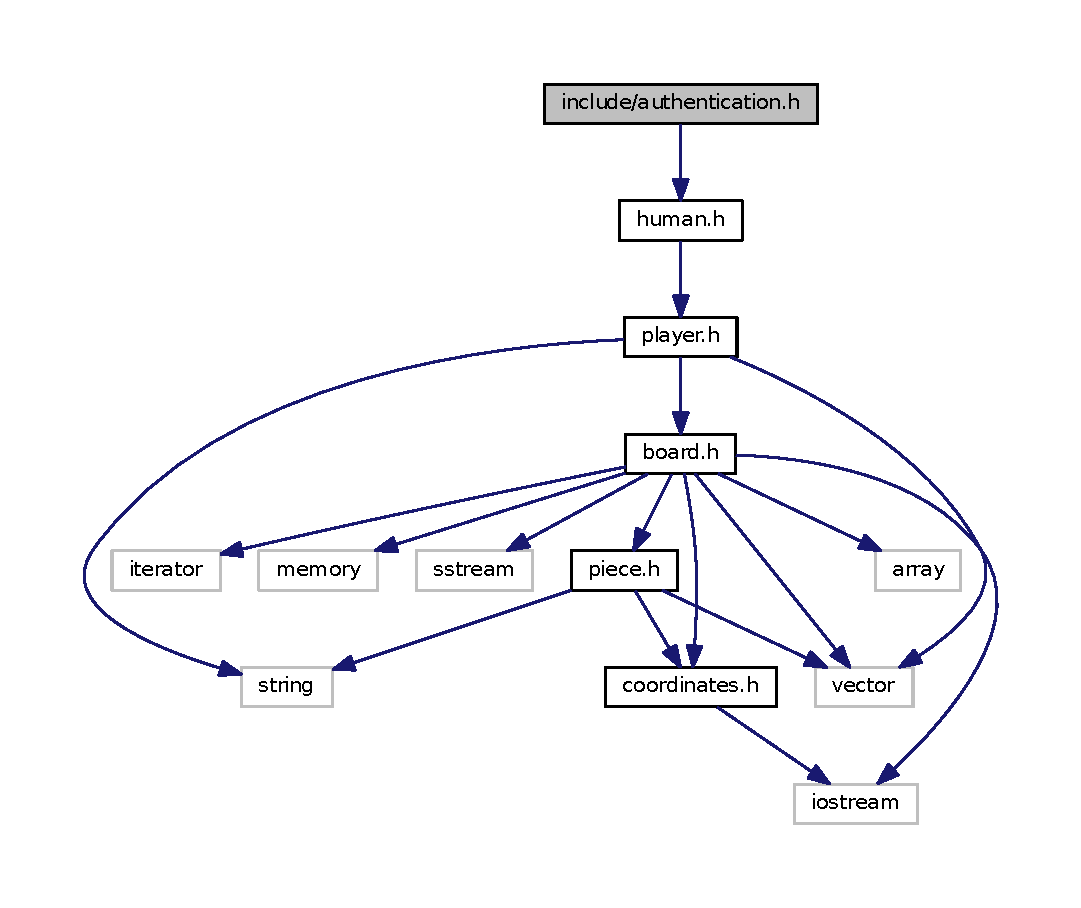
\includegraphics[width=350pt]{authentication_8h__incl}
\end{center}
\end{figure}
This graph shows which files directly or indirectly include this file\+:
\nopagebreak
\begin{figure}[H]
\begin{center}
\leavevmode
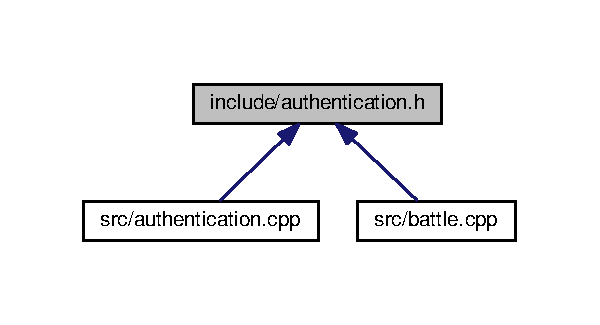
\includegraphics[width=288pt]{authentication_8h__dep__incl}
\end{center}
\end{figure}
\subsection*{Classes}
\begin{DoxyCompactItemize}
\item 
class \hyperlink{classbattle__ship_1_1authentication}{battle\+\_\+ship\+::authentication}
\begin{DoxyCompactList}\small\item\em Class used for login and signup. \end{DoxyCompactList}\end{DoxyCompactItemize}
\subsection*{Namespaces}
\begin{DoxyCompactItemize}
\item 
 \hyperlink{namespacebattle__ship}{battle\+\_\+ship}
\end{DoxyCompactItemize}

\hypertarget{board_8h}{}\section{include/board.h File Reference}
\label{board_8h}\index{include/board.\+h@{include/board.\+h}}
{\ttfamily \#include \char`\"{}coordinates.\+h\char`\"{}}\newline
{\ttfamily \#include \char`\"{}piece.\+h\char`\"{}}\newline
{\ttfamily \#include $<$array$>$}\newline
{\ttfamily \#include $<$iostream$>$}\newline
{\ttfamily \#include $<$iterator$>$}\newline
{\ttfamily \#include $<$memory$>$}\newline
{\ttfamily \#include $<$sstream$>$}\newline
{\ttfamily \#include $<$vector$>$}\newline
Include dependency graph for board.\+h\+:
\nopagebreak
\begin{figure}[H]
\begin{center}
\leavevmode
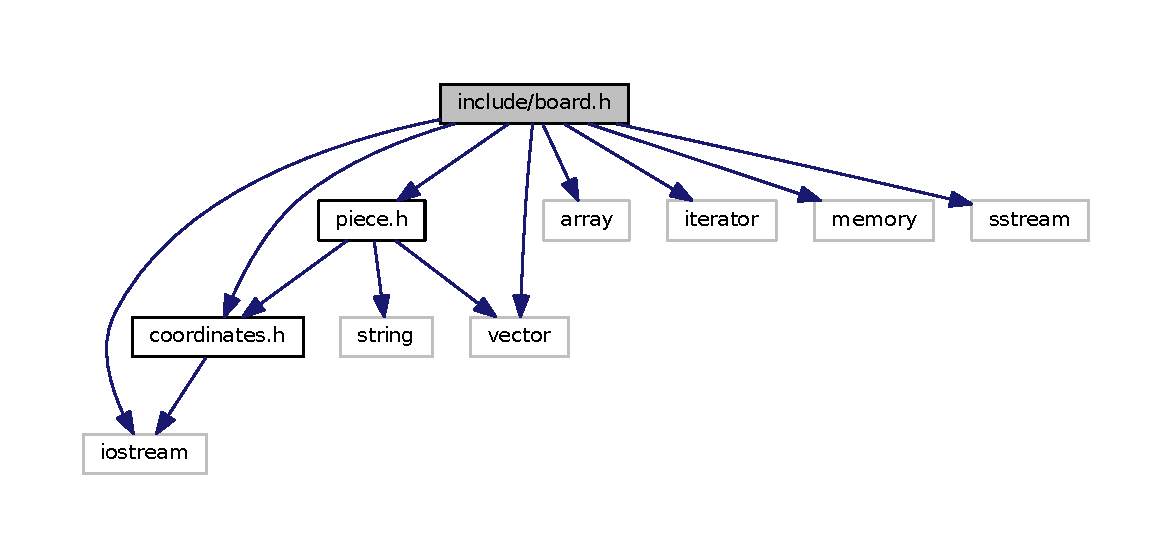
\includegraphics[width=350pt]{board_8h__incl}
\end{center}
\end{figure}
This graph shows which files directly or indirectly include this file\+:
\nopagebreak
\begin{figure}[H]
\begin{center}
\leavevmode
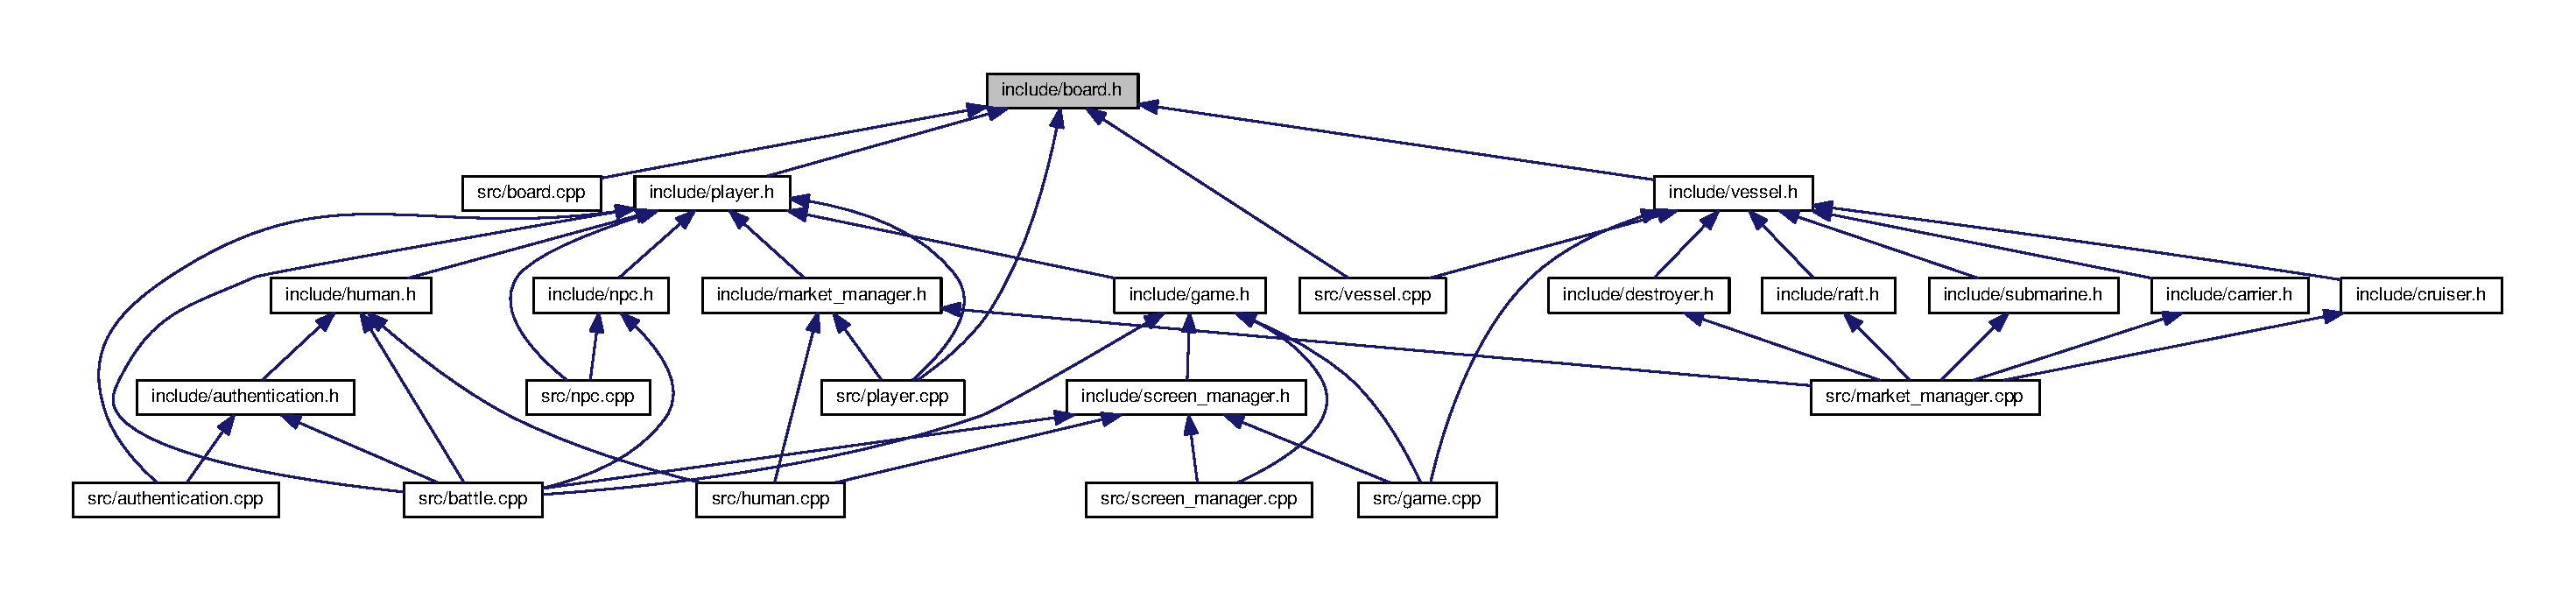
\includegraphics[width=350pt]{board_8h__dep__incl}
\end{center}
\end{figure}
\subsection*{Classes}
\begin{DoxyCompactItemize}
\item 
class \hyperlink{classbattle__ship_1_1board}{battle\+\_\+ship\+::board}
\begin{DoxyCompactList}\small\item\em Class used to handle board state. \end{DoxyCompactList}\end{DoxyCompactItemize}
\subsection*{Namespaces}
\begin{DoxyCompactItemize}
\item 
 \hyperlink{namespacebattle__ship}{battle\+\_\+ship}
\end{DoxyCompactItemize}

\hypertarget{carrier_8h}{}\section{include/carrier.h File Reference}
\label{carrier_8h}\index{include/carrier.\+h@{include/carrier.\+h}}
{\ttfamily \#include \char`\"{}coordinates.\+h\char`\"{}}\newline
{\ttfamily \#include \char`\"{}vessel.\+h\char`\"{}}\newline
{\ttfamily \#include $<$iostream$>$}\newline
Include dependency graph for carrier.\+h\+:
\nopagebreak
\begin{figure}[H]
\begin{center}
\leavevmode
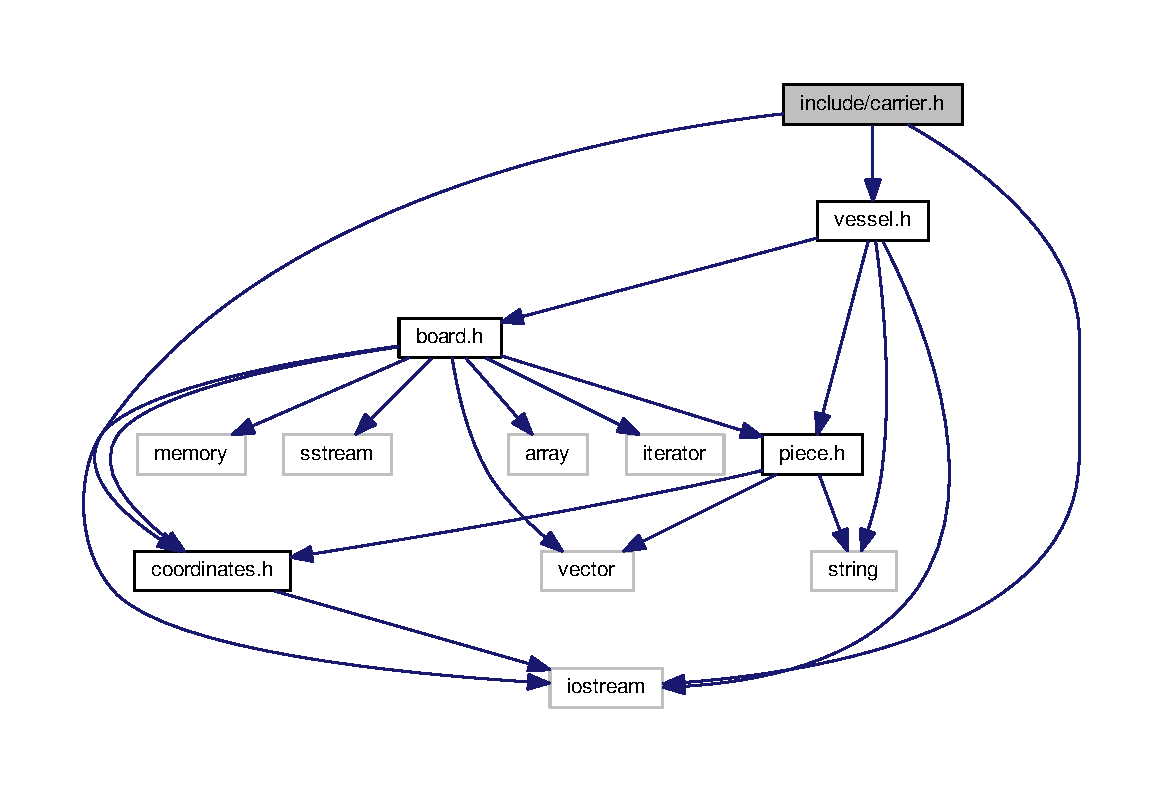
\includegraphics[width=350pt]{carrier_8h__incl}
\end{center}
\end{figure}
This graph shows which files directly or indirectly include this file\+:
\nopagebreak
\begin{figure}[H]
\begin{center}
\leavevmode
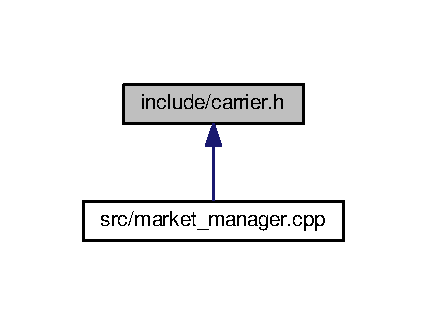
\includegraphics[width=205pt]{carrier_8h__dep__incl}
\end{center}
\end{figure}
\subsection*{Classes}
\begin{DoxyCompactItemize}
\item 
class \hyperlink{classbattle__ship_1_1carrier}{battle\+\_\+ship\+::carrier}
\begin{DoxyCompactList}\small\item\em A type of vessel. \end{DoxyCompactList}\end{DoxyCompactItemize}
\subsection*{Namespaces}
\begin{DoxyCompactItemize}
\item 
 \hyperlink{namespacebattle__ship}{battle\+\_\+ship}
\end{DoxyCompactItemize}

\hypertarget{coordinates_8h}{}\section{include/coordinates.h File Reference}
\label{coordinates_8h}\index{include/coordinates.\+h@{include/coordinates.\+h}}
{\ttfamily \#include $<$iostream$>$}\newline
Include dependency graph for coordinates.\+h\+:\nopagebreak
\begin{figure}[H]
\begin{center}
\leavevmode
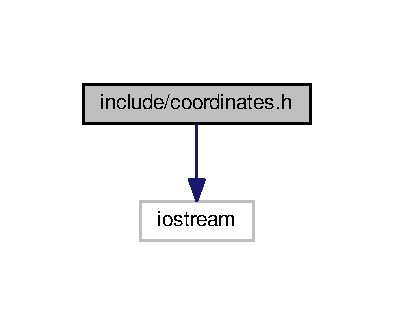
\includegraphics[width=199pt]{coordinates_8h__incl}
\end{center}
\end{figure}
This graph shows which files directly or indirectly include this file\+:
\nopagebreak
\begin{figure}[H]
\begin{center}
\leavevmode
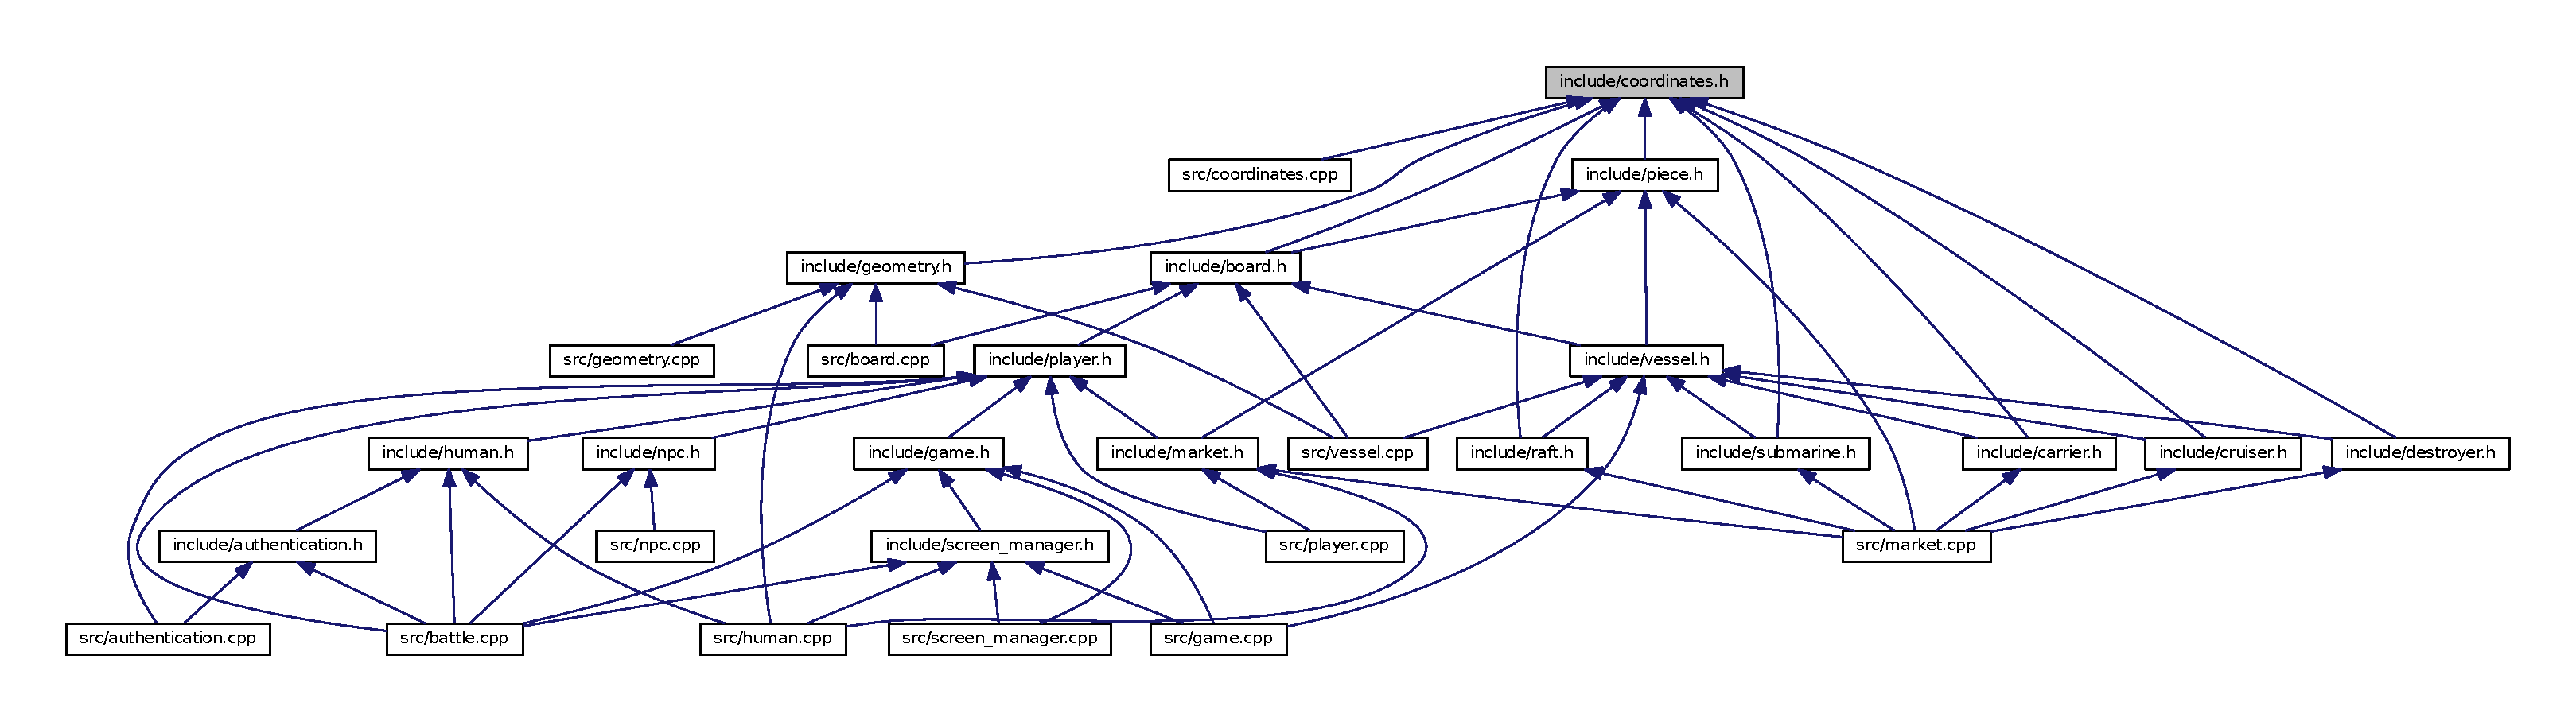
\includegraphics[width=350pt]{coordinates_8h__dep__incl}
\end{center}
\end{figure}
\subsection*{Classes}
\begin{DoxyCompactItemize}
\item 
struct \hyperlink{structbattle__ship_1_1coordinates}{battle\+\_\+ship\+::coordinates}
\end{DoxyCompactItemize}
\subsection*{Namespaces}
\begin{DoxyCompactItemize}
\item 
 \hyperlink{namespacebattle__ship}{battle\+\_\+ship}
\end{DoxyCompactItemize}
\subsection*{Enumerations}
\begin{DoxyCompactItemize}
\item 
enum \hyperlink{namespacebattle__ship_ab3bfa90e413692dac2d4463364f80561}{battle\+\_\+ship\+::x\+\_\+axis} \{ \newline
\hyperlink{namespacebattle__ship_ab3bfa90e413692dac2d4463364f80561a7fc56270e7a70fa81a5935b72eacbe29}{battle\+\_\+ship\+::x\+\_\+axis\+::A} = 1, 
\hyperlink{namespacebattle__ship_ab3bfa90e413692dac2d4463364f80561a9d5ed678fe57bcca610140957afab571}{battle\+\_\+ship\+::x\+\_\+axis\+::B} = 2, 
\hyperlink{namespacebattle__ship_ab3bfa90e413692dac2d4463364f80561a0d61f8370cad1d412f80b84d143e1257}{battle\+\_\+ship\+::x\+\_\+axis\+::C} = 3, 
\hyperlink{namespacebattle__ship_ab3bfa90e413692dac2d4463364f80561af623e75af30e62bbd73d6df5b50bb7b5}{battle\+\_\+ship\+::x\+\_\+axis\+::D} = 4, 
\newline
\hyperlink{namespacebattle__ship_ab3bfa90e413692dac2d4463364f80561a3a3ea00cfc35332cedf6e5e9a32e94da}{battle\+\_\+ship\+::x\+\_\+axis\+::E} = 5, 
\hyperlink{namespacebattle__ship_ab3bfa90e413692dac2d4463364f80561a800618943025315f869e4e1f09471012}{battle\+\_\+ship\+::x\+\_\+axis\+::F} = 6, 
\hyperlink{namespacebattle__ship_ab3bfa90e413692dac2d4463364f80561adfcf28d0734569a6a693bc8194de62bf}{battle\+\_\+ship\+::x\+\_\+axis\+::G} = 7, 
\hyperlink{namespacebattle__ship_ab3bfa90e413692dac2d4463364f80561ac1d9f50f86825a1a2302ec2449c17196}{battle\+\_\+ship\+::x\+\_\+axis\+::H} = 8, 
\newline
\hyperlink{namespacebattle__ship_ab3bfa90e413692dac2d4463364f80561add7536794b63bf90eccfd37f9b147d7f}{battle\+\_\+ship\+::x\+\_\+axis\+::I} = 9, 
\hyperlink{namespacebattle__ship_ab3bfa90e413692dac2d4463364f80561aff44570aca8241914870afbc310cdb85}{battle\+\_\+ship\+::x\+\_\+axis\+::J} = 10
 \}
\item 
enum \hyperlink{namespacebattle__ship_aed87488f0a73f0d0679fe343fb61c784}{battle\+\_\+ship\+::orientation} \{ \hyperlink{namespacebattle__ship_aed87488f0a73f0d0679fe343fb61c784a4505cad087312551a6fbbe6ebe163e0f}{battle\+\_\+ship\+::orientation\+::horizontal}, 
\hyperlink{namespacebattle__ship_aed87488f0a73f0d0679fe343fb61c784ae6dec152d6a941fccb0a5e8cc2579cc3}{battle\+\_\+ship\+::orientation\+::vertical}
 \}
\end{DoxyCompactItemize}

\hypertarget{cruiser_8h}{}\section{include/cruiser.h File Reference}
\label{cruiser_8h}\index{include/cruiser.\+h@{include/cruiser.\+h}}
{\ttfamily \#include \char`\"{}coordinates.\+h\char`\"{}}\newline
{\ttfamily \#include \char`\"{}vessel.\+h\char`\"{}}\newline
{\ttfamily \#include $<$iostream$>$}\newline
Include dependency graph for cruiser.\+h\+:
\nopagebreak
\begin{figure}[H]
\begin{center}
\leavevmode
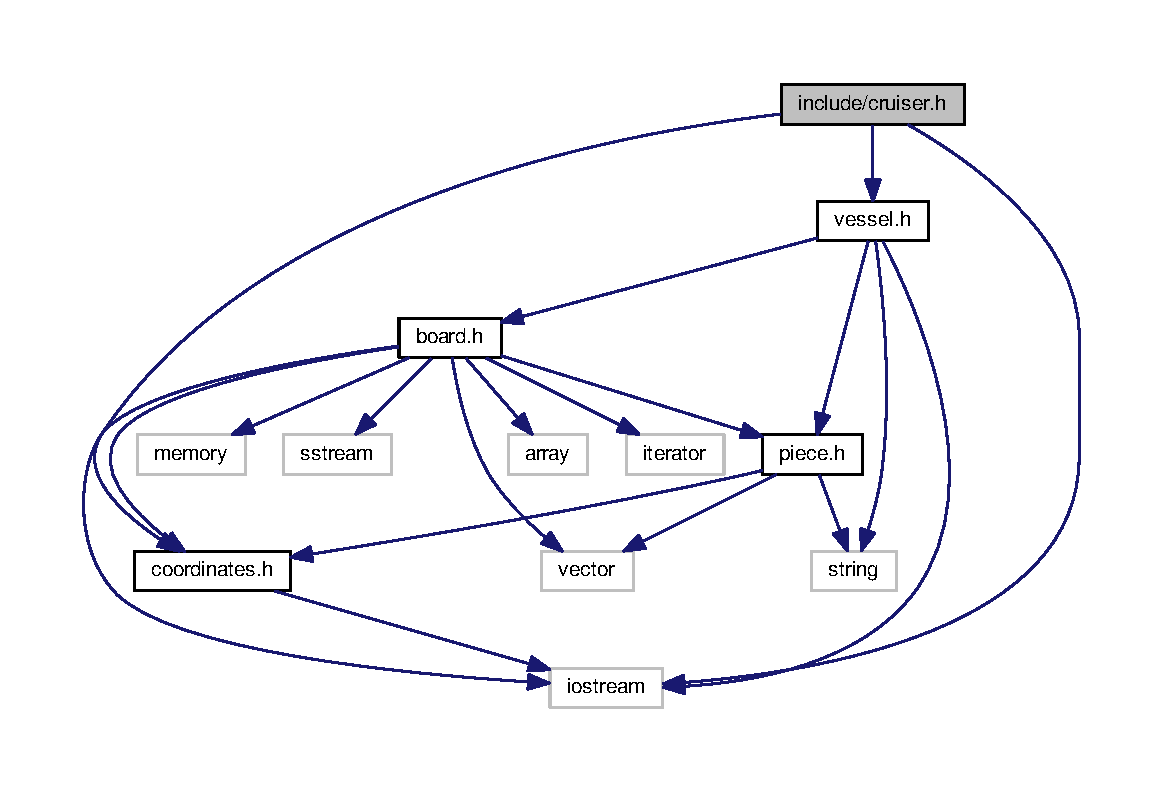
\includegraphics[width=350pt]{cruiser_8h__incl}
\end{center}
\end{figure}
This graph shows which files directly or indirectly include this file\+:
\nopagebreak
\begin{figure}[H]
\begin{center}
\leavevmode
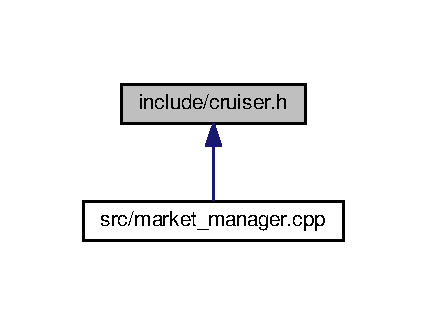
\includegraphics[width=205pt]{cruiser_8h__dep__incl}
\end{center}
\end{figure}
\subsection*{Classes}
\begin{DoxyCompactItemize}
\item 
class \hyperlink{classbattle__ship_1_1cruiser}{battle\+\_\+ship\+::cruiser}
\begin{DoxyCompactList}\small\item\em A type of vessel. \end{DoxyCompactList}\end{DoxyCompactItemize}
\subsection*{Namespaces}
\begin{DoxyCompactItemize}
\item 
 \hyperlink{namespacebattle__ship}{battle\+\_\+ship}
\end{DoxyCompactItemize}

\hypertarget{destroyer_8h}{}\section{include/destroyer.h File Reference}
\label{destroyer_8h}\index{include/destroyer.\+h@{include/destroyer.\+h}}
{\ttfamily \#include \char`\"{}coordinates.\+h\char`\"{}}\newline
{\ttfamily \#include \char`\"{}vessel.\+h\char`\"{}}\newline
{\ttfamily \#include $<$iostream$>$}\newline
Include dependency graph for destroyer.\+h\+:
\nopagebreak
\begin{figure}[H]
\begin{center}
\leavevmode
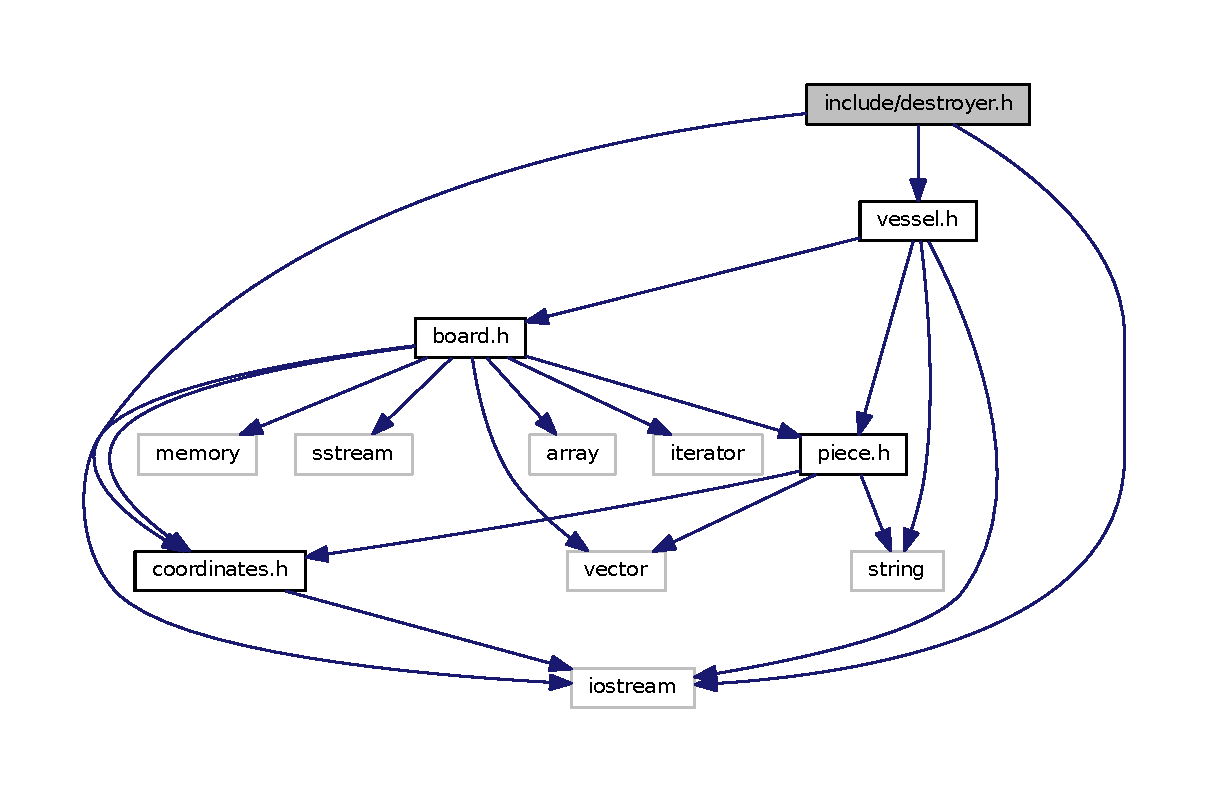
\includegraphics[width=350pt]{destroyer_8h__incl}
\end{center}
\end{figure}
This graph shows which files directly or indirectly include this file\+:
\nopagebreak
\begin{figure}[H]
\begin{center}
\leavevmode
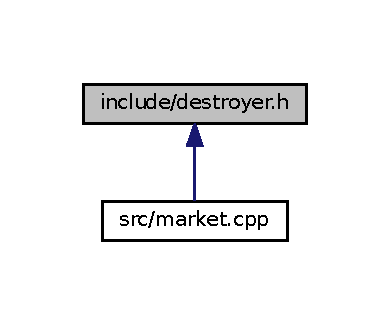
\includegraphics[width=205pt]{destroyer_8h__dep__incl}
\end{center}
\end{figure}
\subsection*{Classes}
\begin{DoxyCompactItemize}
\item 
class \hyperlink{classbattle__ship_1_1destroyer}{battle\+\_\+ship\+::destroyer}
\begin{DoxyCompactList}\small\item\em A type of vessel. \end{DoxyCompactList}\end{DoxyCompactItemize}
\subsection*{Namespaces}
\begin{DoxyCompactItemize}
\item 
 \hyperlink{namespacebattle__ship}{battle\+\_\+ship}
\end{DoxyCompactItemize}

\hypertarget{game_8h}{}\section{include/game.h File Reference}
\label{game_8h}\index{include/game.\+h@{include/game.\+h}}
{\ttfamily \#include \char`\"{}player.\+h\char`\"{}}\newline
{\ttfamily \#include \char`\"{}rules.\+h\char`\"{}}\newline
Include dependency graph for game.\+h\+:
\nopagebreak
\begin{figure}[H]
\begin{center}
\leavevmode
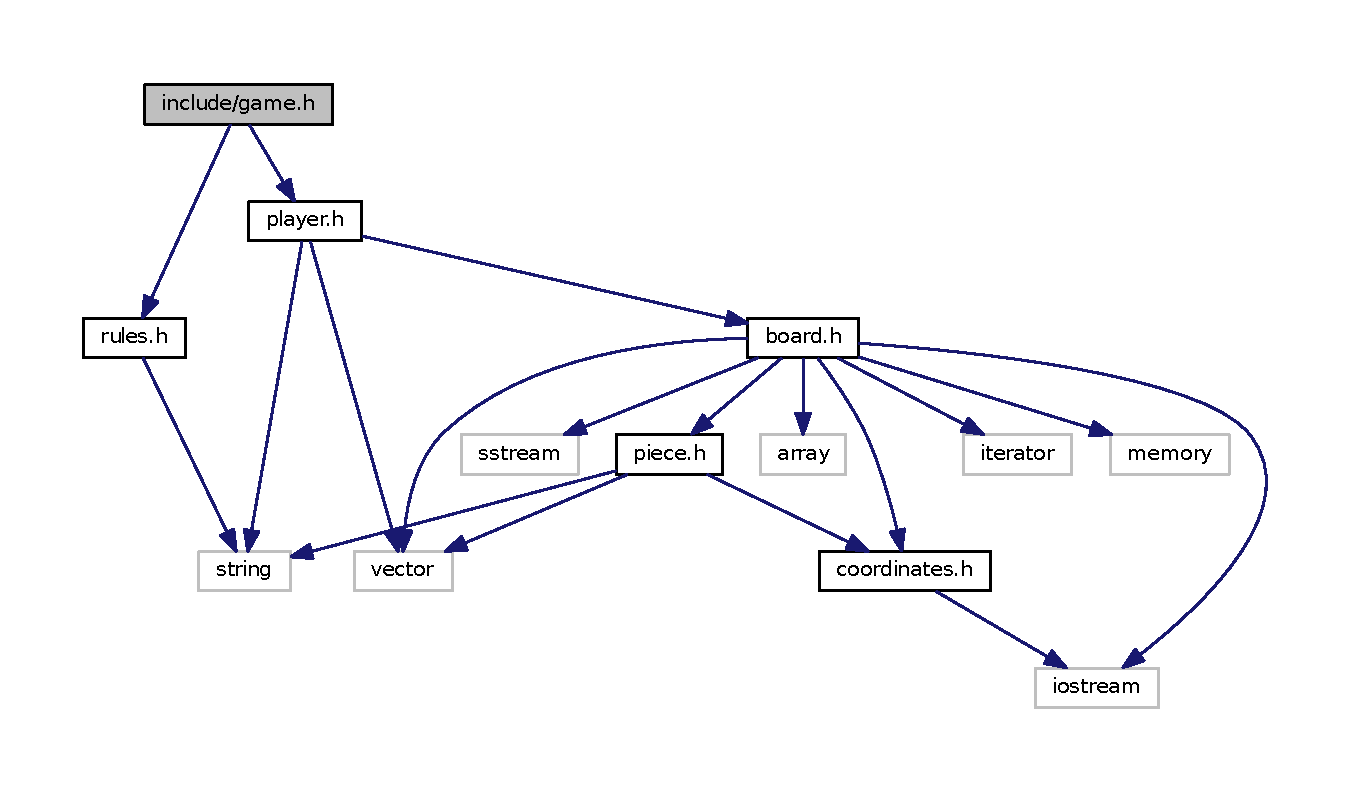
\includegraphics[width=350pt]{game_8h__incl}
\end{center}
\end{figure}
This graph shows which files directly or indirectly include this file\+:
\nopagebreak
\begin{figure}[H]
\begin{center}
\leavevmode
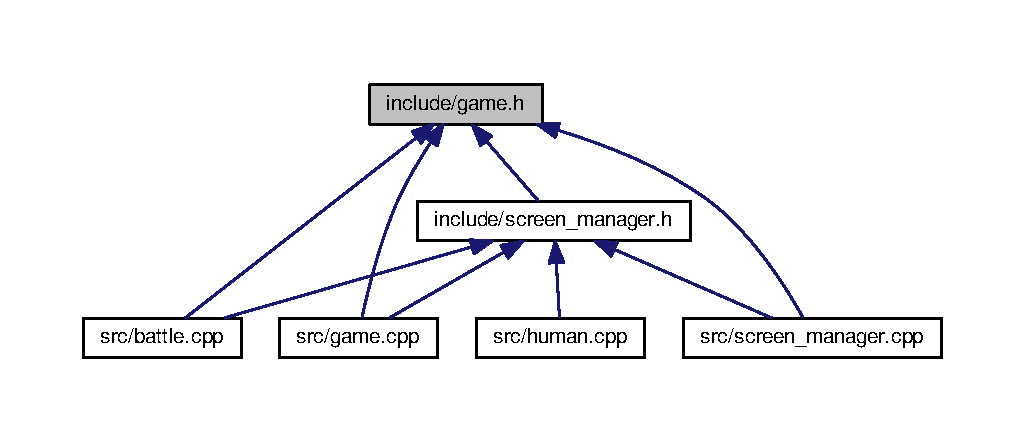
\includegraphics[width=350pt]{game_8h__dep__incl}
\end{center}
\end{figure}
\subsection*{Classes}
\begin{DoxyCompactItemize}
\item 
class \hyperlink{classbattle__ship_1_1game}{battle\+\_\+ship\+::game}
\end{DoxyCompactItemize}
\subsection*{Namespaces}
\begin{DoxyCompactItemize}
\item 
 \hyperlink{namespacebattle__ship}{battle\+\_\+ship}
\end{DoxyCompactItemize}

\hypertarget{geometry_8h}{}\section{include/geometry.h File Reference}
\label{geometry_8h}\index{include/geometry.\+h@{include/geometry.\+h}}
{\ttfamily \#include \char`\"{}coordinates.\+h\char`\"{}}\newline
{\ttfamily \#include $<$string$>$}\newline
Include dependency graph for geometry.\+h\+:
\nopagebreak
\begin{figure}[H]
\begin{center}
\leavevmode
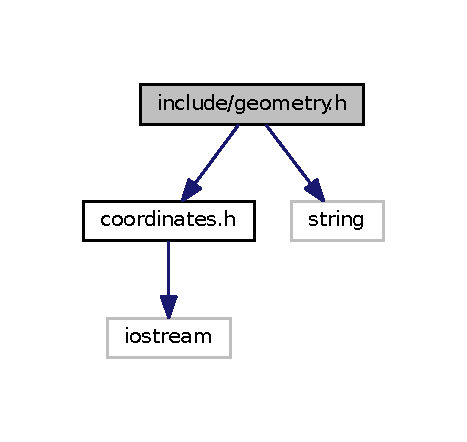
\includegraphics[width=224pt]{geometry_8h__incl}
\end{center}
\end{figure}
This graph shows which files directly or indirectly include this file\+:
\nopagebreak
\begin{figure}[H]
\begin{center}
\leavevmode
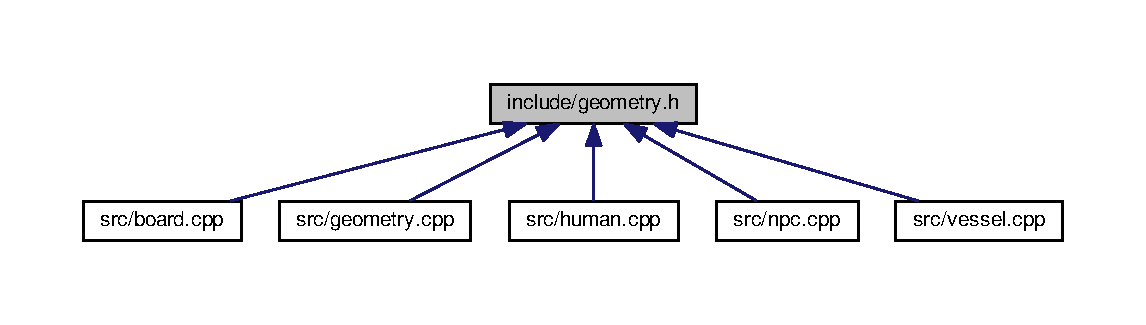
\includegraphics[width=350pt]{geometry_8h__dep__incl}
\end{center}
\end{figure}
\subsection*{Classes}
\begin{DoxyCompactItemize}
\item 
class \hyperlink{classbattle__ship_1_1geometry}{battle\+\_\+ship\+::geometry}
\end{DoxyCompactItemize}
\subsection*{Namespaces}
\begin{DoxyCompactItemize}
\item 
 \hyperlink{namespacebattle__ship}{battle\+\_\+ship}
\end{DoxyCompactItemize}

\hypertarget{highscore__manager_8h}{}\section{include/highscore\+\_\+manager.h File Reference}
\label{highscore__manager_8h}\index{include/highscore\+\_\+manager.\+h@{include/highscore\+\_\+manager.\+h}}
{\ttfamily \#include $<$string$>$}\newline
{\ttfamily \#include $<$tuple$>$}\newline
{\ttfamily \#include $<$vector$>$}\newline
Include dependency graph for highscore\+\_\+manager.\+h\+:
\nopagebreak
\begin{figure}[H]
\begin{center}
\leavevmode
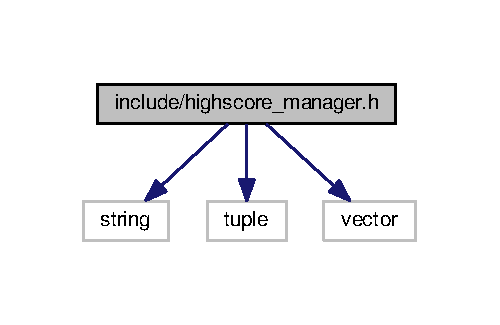
\includegraphics[width=249pt]{highscore__manager_8h__incl}
\end{center}
\end{figure}
This graph shows which files directly or indirectly include this file\+:
\nopagebreak
\begin{figure}[H]
\begin{center}
\leavevmode
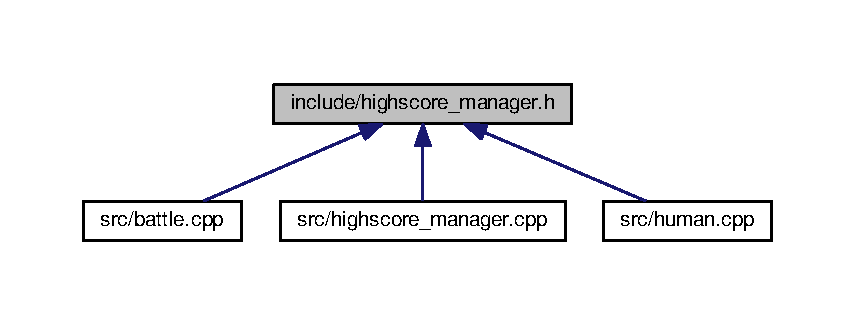
\includegraphics[width=330pt]{highscore__manager_8h__dep__incl}
\end{center}
\end{figure}
\subsection*{Classes}
\begin{DoxyCompactItemize}
\item 
class \hyperlink{classbattle__ship_1_1highscore__manager}{battle\+\_\+ship\+::highscore\+\_\+manager}
\end{DoxyCompactItemize}
\subsection*{Namespaces}
\begin{DoxyCompactItemize}
\item 
 \hyperlink{namespacebattle__ship}{battle\+\_\+ship}
\end{DoxyCompactItemize}

\hypertarget{human_8h}{}\section{include/human.h File Reference}
\label{human_8h}\index{include/human.\+h@{include/human.\+h}}
{\ttfamily \#include \char`\"{}player.\+h\char`\"{}}\newline
Include dependency graph for human.\+h\+:
\nopagebreak
\begin{figure}[H]
\begin{center}
\leavevmode
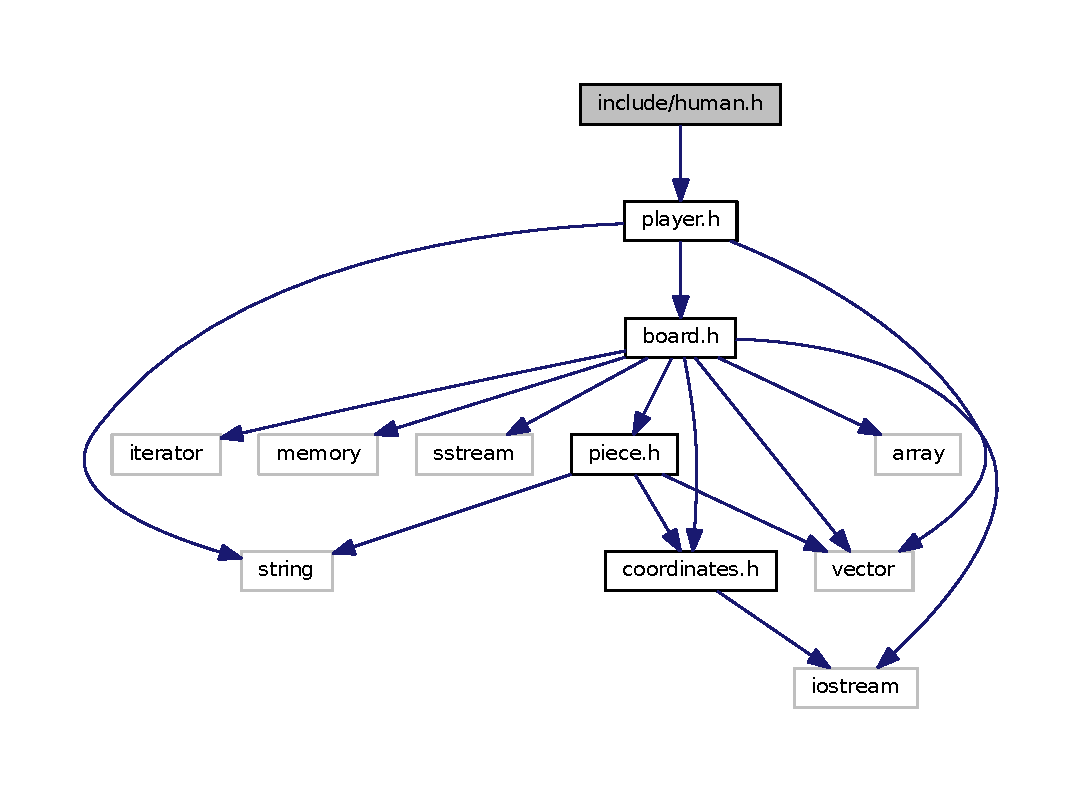
\includegraphics[width=350pt]{human_8h__incl}
\end{center}
\end{figure}
This graph shows which files directly or indirectly include this file\+:
\nopagebreak
\begin{figure}[H]
\begin{center}
\leavevmode
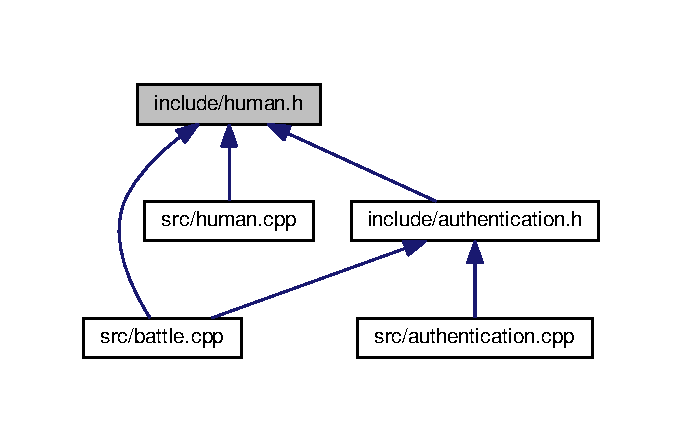
\includegraphics[width=328pt]{human_8h__dep__incl}
\end{center}
\end{figure}
\subsection*{Classes}
\begin{DoxyCompactItemize}
\item 
class \hyperlink{classbattle__ship_1_1human}{battle\+\_\+ship\+::human}
\begin{DoxyCompactList}\small\item\em A type of player Implements methods targeted for playable characters (human controlled) \end{DoxyCompactList}\end{DoxyCompactItemize}
\subsection*{Namespaces}
\begin{DoxyCompactItemize}
\item 
 \hyperlink{namespacebattle__ship}{battle\+\_\+ship}
\end{DoxyCompactItemize}

\hypertarget{market__manager_8h}{}\section{include/market\+\_\+manager.h File Reference}
\label{market__manager_8h}\index{include/market\+\_\+manager.\+h@{include/market\+\_\+manager.\+h}}
{\ttfamily \#include \char`\"{}piece.\+h\char`\"{}}\newline
{\ttfamily \#include \char`\"{}player.\+h\char`\"{}}\newline
{\ttfamily \#include $<$string$>$}\newline
{\ttfamily \#include $<$tuple$>$}\newline
{\ttfamily \#include $<$vector$>$}\newline
Include dependency graph for market\+\_\+manager.\+h\+:
\nopagebreak
\begin{figure}[H]
\begin{center}
\leavevmode
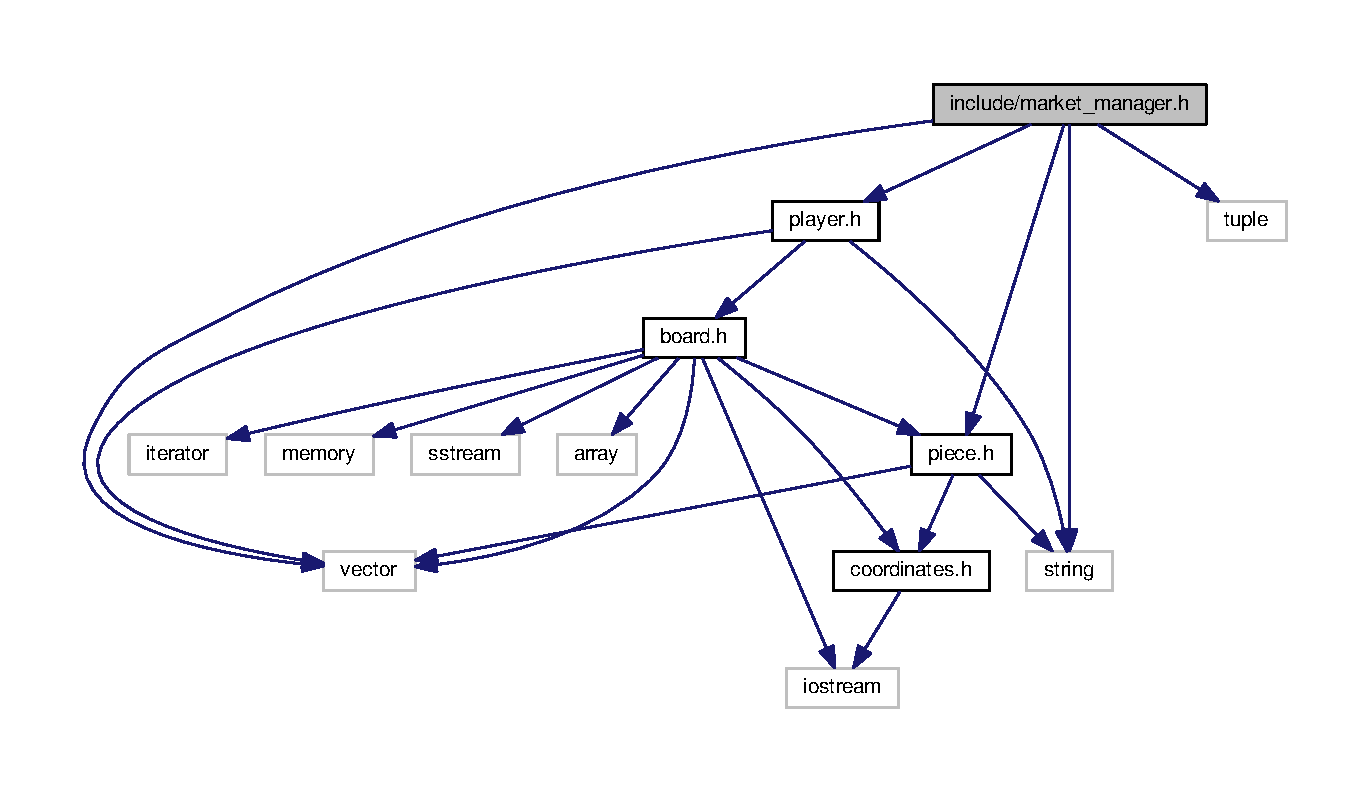
\includegraphics[width=350pt]{market__manager_8h__incl}
\end{center}
\end{figure}
This graph shows which files directly or indirectly include this file\+:
\nopagebreak
\begin{figure}[H]
\begin{center}
\leavevmode
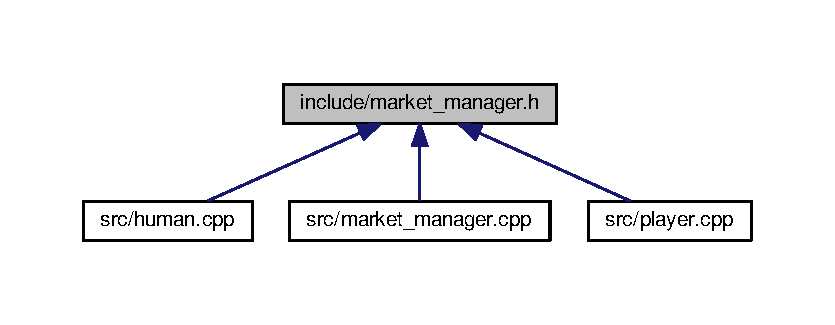
\includegraphics[width=350pt]{market__manager_8h__dep__incl}
\end{center}
\end{figure}
\subsection*{Classes}
\begin{DoxyCompactItemize}
\item 
class \hyperlink{classbattle__ship_1_1market__manager}{battle\+\_\+ship\+::market\+\_\+manager}
\begin{DoxyCompactList}\small\item\em Used to manage available vessels and transactions via budget checking. \end{DoxyCompactList}\end{DoxyCompactItemize}
\subsection*{Namespaces}
\begin{DoxyCompactItemize}
\item 
 \hyperlink{namespacebattle__ship}{battle\+\_\+ship}
\end{DoxyCompactItemize}

\hypertarget{notification__manager_8h}{}\section{include/notification\+\_\+manager.h File Reference}
\label{notification__manager_8h}\index{include/notification\+\_\+manager.\+h@{include/notification\+\_\+manager.\+h}}
{\ttfamily \#include $<$iostream$>$}\newline
{\ttfamily \#include $<$string$>$}\newline
{\ttfamily \#include $<$vector$>$}\newline
Include dependency graph for notification\+\_\+manager.\+h\+:
\nopagebreak
\begin{figure}[H]
\begin{center}
\leavevmode
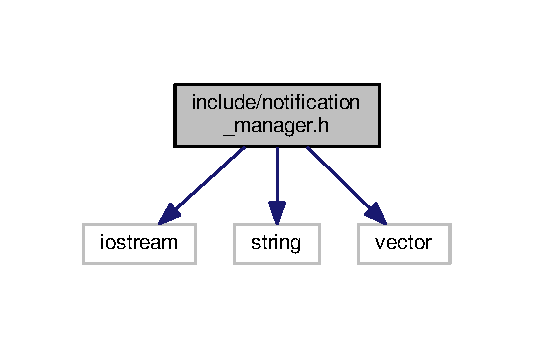
\includegraphics[width=267pt]{notification__manager_8h__incl}
\end{center}
\end{figure}
This graph shows which files directly or indirectly include this file\+:
\nopagebreak
\begin{figure}[H]
\begin{center}
\leavevmode
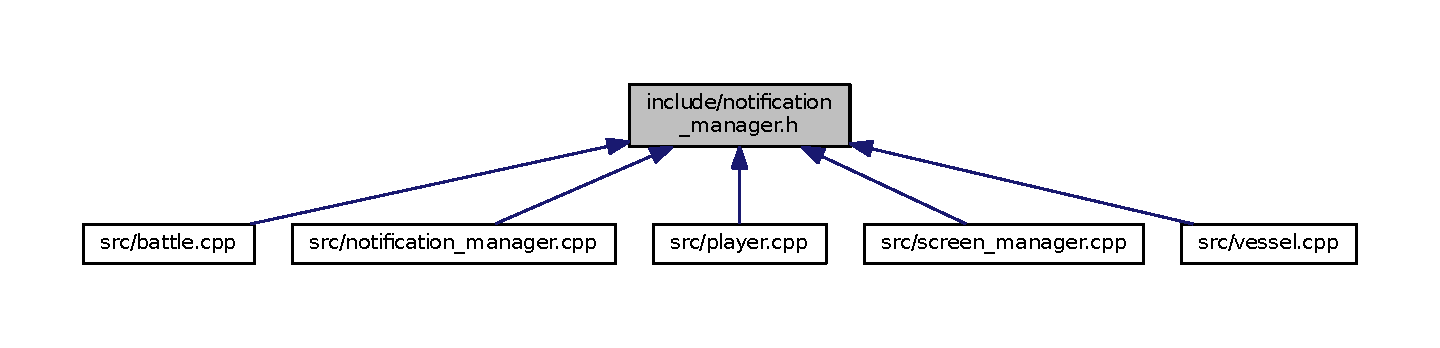
\includegraphics[width=350pt]{notification__manager_8h__dep__incl}
\end{center}
\end{figure}
\subsection*{Classes}
\begin{DoxyCompactItemize}
\item 
class \hyperlink{classbattle__ship_1_1notification__manager}{battle\+\_\+ship\+::notification\+\_\+manager}
\end{DoxyCompactItemize}
\subsection*{Namespaces}
\begin{DoxyCompactItemize}
\item 
 \hyperlink{namespacebattle__ship}{battle\+\_\+ship}
\end{DoxyCompactItemize}

\hypertarget{npc_8h}{}\section{include/npc.h File Reference}
\label{npc_8h}\index{include/npc.\+h@{include/npc.\+h}}
{\ttfamily \#include \char`\"{}player.\+h\char`\"{}}\newline
{\ttfamily \#include $<$string$>$}\newline
Include dependency graph for npc.\+h\+:
\nopagebreak
\begin{figure}[H]
\begin{center}
\leavevmode
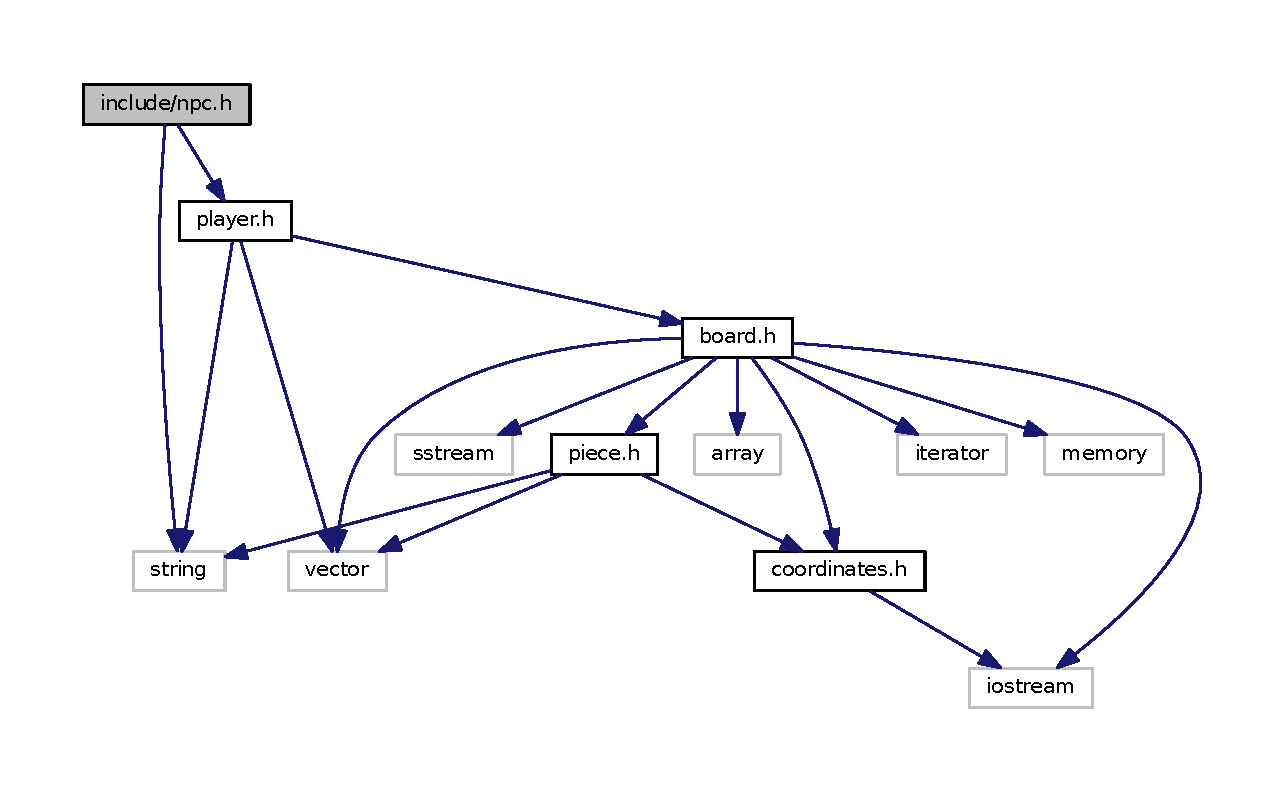
\includegraphics[width=350pt]{npc_8h__incl}
\end{center}
\end{figure}
This graph shows which files directly or indirectly include this file\+:
\nopagebreak
\begin{figure}[H]
\begin{center}
\leavevmode
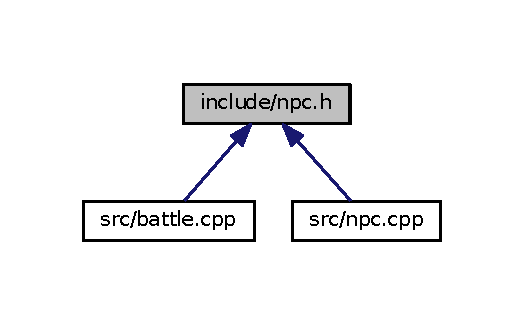
\includegraphics[width=252pt]{npc_8h__dep__incl}
\end{center}
\end{figure}
\subsection*{Classes}
\begin{DoxyCompactItemize}
\item 
class \hyperlink{classbattle__ship_1_1npc}{battle\+\_\+ship\+::npc}
\end{DoxyCompactItemize}
\subsection*{Namespaces}
\begin{DoxyCompactItemize}
\item 
 \hyperlink{namespacebattle__ship}{battle\+\_\+ship}
\end{DoxyCompactItemize}

\hypertarget{piece_8h}{}\section{include/piece.h File Reference}
\label{piece_8h}\index{include/piece.\+h@{include/piece.\+h}}
{\ttfamily \#include \char`\"{}coordinates.\+h\char`\"{}}\newline
{\ttfamily \#include $<$string$>$}\newline
{\ttfamily \#include $<$vector$>$}\newline
Include dependency graph for piece.\+h\+:
\nopagebreak
\begin{figure}[H]
\begin{center}
\leavevmode
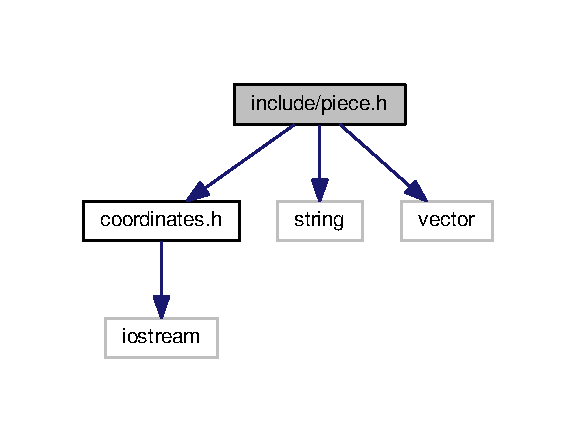
\includegraphics[width=290pt]{piece_8h__incl}
\end{center}
\end{figure}
This graph shows which files directly or indirectly include this file\+:
\nopagebreak
\begin{figure}[H]
\begin{center}
\leavevmode
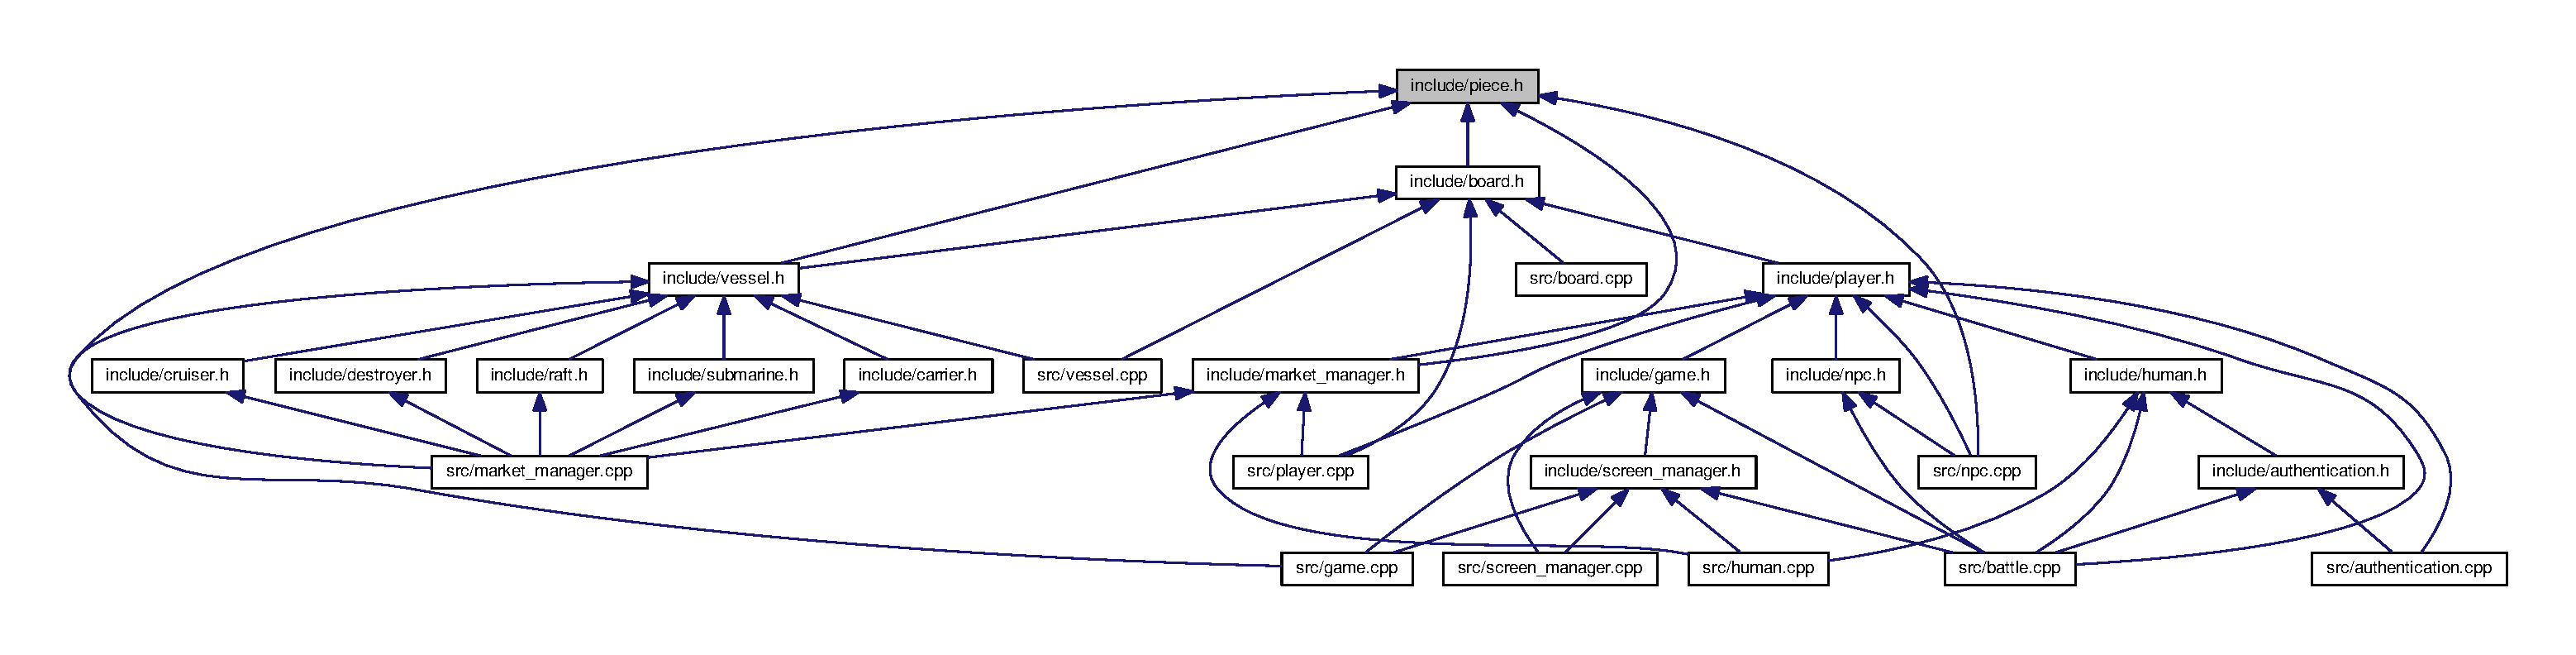
\includegraphics[width=350pt]{piece_8h__dep__incl}
\end{center}
\end{figure}
\subsection*{Classes}
\begin{DoxyCompactItemize}
\item 
class \hyperlink{classbattle__ship_1_1piece}{battle\+\_\+ship\+::piece}
\end{DoxyCompactItemize}
\subsection*{Namespaces}
\begin{DoxyCompactItemize}
\item 
 \hyperlink{namespacebattle__ship}{battle\+\_\+ship}
\end{DoxyCompactItemize}

\hypertarget{player_8h}{}\section{include/player.h File Reference}
\label{player_8h}\index{include/player.\+h@{include/player.\+h}}
{\ttfamily \#include \char`\"{}board.\+h\char`\"{}}\newline
{\ttfamily \#include $<$string$>$}\newline
{\ttfamily \#include $<$vector$>$}\newline
Include dependency graph for player.\+h\+:
\nopagebreak
\begin{figure}[H]
\begin{center}
\leavevmode
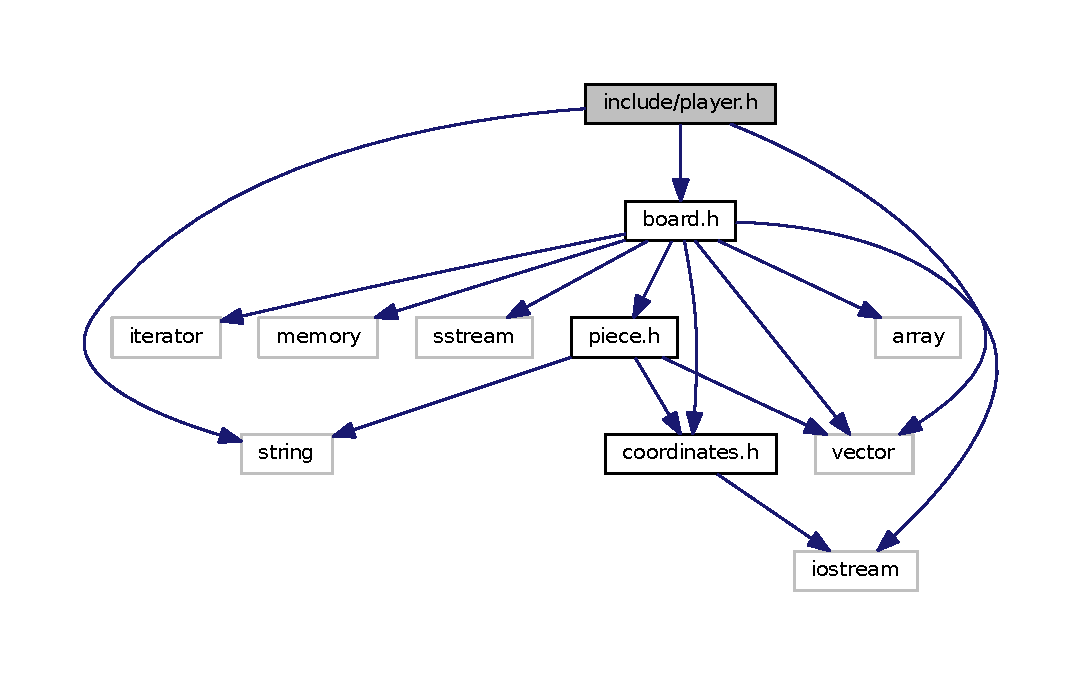
\includegraphics[width=350pt]{player_8h__incl}
\end{center}
\end{figure}
This graph shows which files directly or indirectly include this file\+:
\nopagebreak
\begin{figure}[H]
\begin{center}
\leavevmode
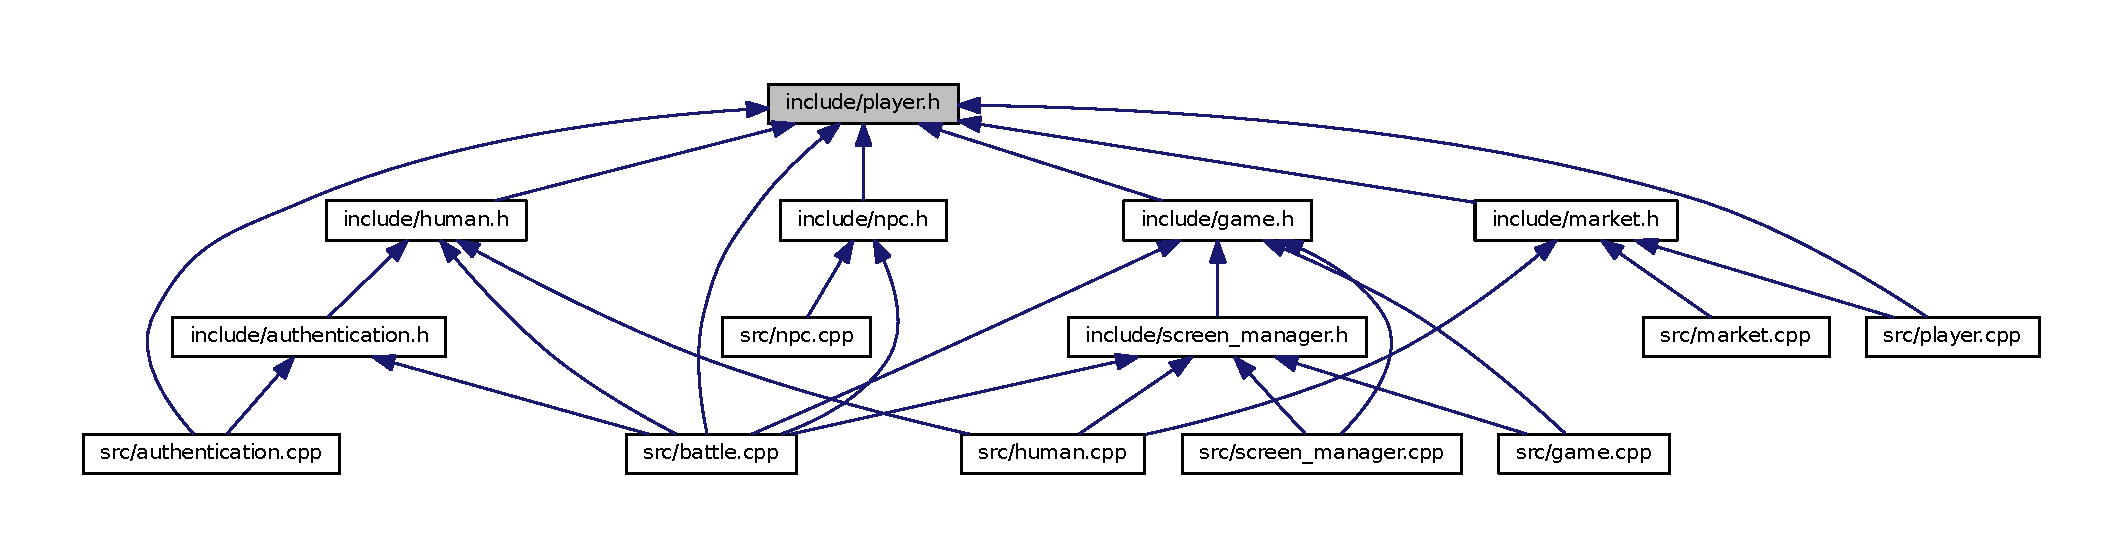
\includegraphics[width=350pt]{player_8h__dep__incl}
\end{center}
\end{figure}
\subsection*{Classes}
\begin{DoxyCompactItemize}
\item 
class \hyperlink{classbattle__ship_1_1player}{battle\+\_\+ship\+::player}
\begin{DoxyCompactList}\small\item\em Abstract class for a player. \end{DoxyCompactList}\end{DoxyCompactItemize}
\subsection*{Namespaces}
\begin{DoxyCompactItemize}
\item 
 \hyperlink{namespacebattle__ship}{battle\+\_\+ship}
\end{DoxyCompactItemize}

\hypertarget{raft_8h}{}\section{include/raft.h File Reference}
\label{raft_8h}\index{include/raft.\+h@{include/raft.\+h}}
{\ttfamily \#include \char`\"{}coordinates.\+h\char`\"{}}\newline
{\ttfamily \#include \char`\"{}vessel.\+h\char`\"{}}\newline
{\ttfamily \#include $<$iostream$>$}\newline
Include dependency graph for raft.\+h\+:
\nopagebreak
\begin{figure}[H]
\begin{center}
\leavevmode
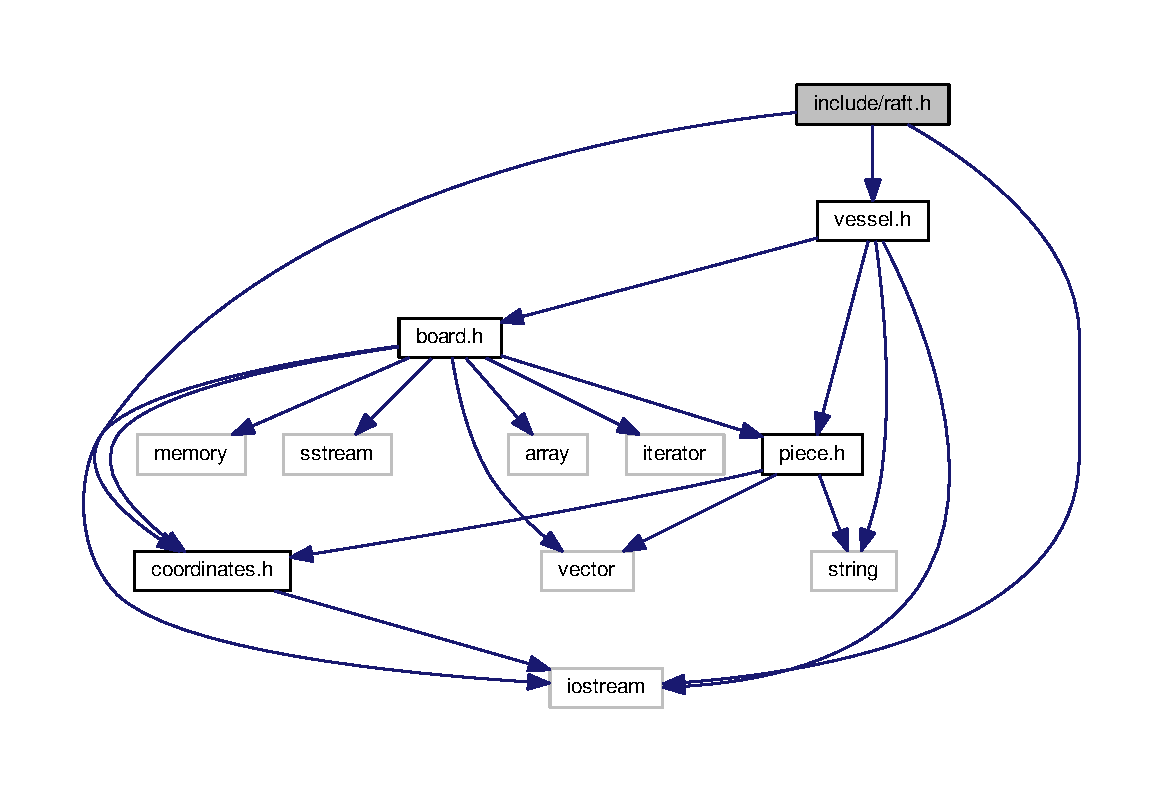
\includegraphics[width=350pt]{raft_8h__incl}
\end{center}
\end{figure}
This graph shows which files directly or indirectly include this file\+:
\nopagebreak
\begin{figure}[H]
\begin{center}
\leavevmode
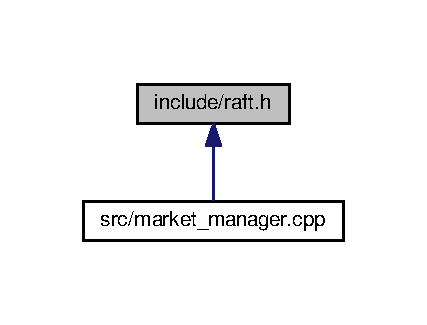
\includegraphics[width=205pt]{raft_8h__dep__incl}
\end{center}
\end{figure}
\subsection*{Classes}
\begin{DoxyCompactItemize}
\item 
class \hyperlink{classbattle__ship_1_1raft}{battle\+\_\+ship\+::raft}
\begin{DoxyCompactList}\small\item\em A type of vessel. \end{DoxyCompactList}\end{DoxyCompactItemize}
\subsection*{Namespaces}
\begin{DoxyCompactItemize}
\item 
 \hyperlink{namespacebattle__ship}{battle\+\_\+ship}
\end{DoxyCompactItemize}

\hypertarget{screen__manager_8h}{}\section{include/screen\+\_\+manager.h File Reference}
\label{screen__manager_8h}\index{include/screen\+\_\+manager.\+h@{include/screen\+\_\+manager.\+h}}
{\ttfamily \#include \char`\"{}game.\+h\char`\"{}}\newline
{\ttfamily \#include $<$iostream$>$}\newline
Include dependency graph for screen\+\_\+manager.\+h\+:\nopagebreak
\begin{figure}[H]
\begin{center}
\leavevmode
\includegraphics[width=350pt]{screen__manager_8h__incl}
\end{center}
\end{figure}
This graph shows which files directly or indirectly include this file\+:
\nopagebreak
\begin{figure}[H]
\begin{center}
\leavevmode
\includegraphics[width=350pt]{screen__manager_8h__dep__incl}
\end{center}
\end{figure}
\subsection*{Classes}
\begin{DoxyCompactItemize}
\item 
class \hyperlink{classbattle__ship_1_1screen__manager}{battle\+\_\+ship\+::screen\+\_\+manager}
\end{DoxyCompactItemize}
\subsection*{Namespaces}
\begin{DoxyCompactItemize}
\item 
 \hyperlink{namespacebattle__ship}{battle\+\_\+ship}
\end{DoxyCompactItemize}

\hypertarget{submarine_8h}{}\section{include/submarine.h File Reference}
\label{submarine_8h}\index{include/submarine.\+h@{include/submarine.\+h}}
{\ttfamily \#include \char`\"{}coordinates.\+h\char`\"{}}\newline
{\ttfamily \#include \char`\"{}vessel.\+h\char`\"{}}\newline
{\ttfamily \#include $<$iostream$>$}\newline
Include dependency graph for submarine.\+h\+:
\nopagebreak
\begin{figure}[H]
\begin{center}
\leavevmode
\includegraphics[width=350pt]{submarine_8h__incl}
\end{center}
\end{figure}
This graph shows which files directly or indirectly include this file\+:
\nopagebreak
\begin{figure}[H]
\begin{center}
\leavevmode
\includegraphics[width=193pt]{submarine_8h__dep__incl}
\end{center}
\end{figure}
\subsection*{Classes}
\begin{DoxyCompactItemize}
\item 
class \hyperlink{classbattle__ship_1_1submarine}{battle\+\_\+ship\+::submarine}
\end{DoxyCompactItemize}
\subsection*{Namespaces}
\begin{DoxyCompactItemize}
\item 
 \hyperlink{namespacebattle__ship}{battle\+\_\+ship}
\end{DoxyCompactItemize}

\hypertarget{vessel_8h}{}\section{include/vessel.h File Reference}
\label{vessel_8h}\index{include/vessel.\+h@{include/vessel.\+h}}
{\ttfamily \#include \char`\"{}board.\+h\char`\"{}}\newline
{\ttfamily \#include \char`\"{}piece.\+h\char`\"{}}\newline
{\ttfamily \#include $<$iostream$>$}\newline
{\ttfamily \#include $<$string$>$}\newline
Include dependency graph for vessel.\+h\+:
\nopagebreak
\begin{figure}[H]
\begin{center}
\leavevmode
\includegraphics[width=350pt]{vessel_8h__incl}
\end{center}
\end{figure}
This graph shows which files directly or indirectly include this file\+:
\nopagebreak
\begin{figure}[H]
\begin{center}
\leavevmode
\includegraphics[width=350pt]{vessel_8h__dep__incl}
\end{center}
\end{figure}
\subsection*{Classes}
\begin{DoxyCompactItemize}
\item 
class \hyperlink{classbattle__ship_1_1vessel}{battle\+\_\+ship\+::vessel}
\begin{DoxyCompactList}\small\item\em Implements the methods for the abstract piece class. \end{DoxyCompactList}\end{DoxyCompactItemize}
\subsection*{Namespaces}
\begin{DoxyCompactItemize}
\item 
 \hyperlink{namespacebattle__ship}{battle\+\_\+ship}
\end{DoxyCompactItemize}

\hypertarget{authentication_8cpp}{}\section{src/authentication.cpp File Reference}
\label{authentication_8cpp}\index{src/authentication.\+cpp@{src/authentication.\+cpp}}
{\ttfamily \#include \char`\"{}authentication.\+h\char`\"{}}\newline
{\ttfamily \#include \char`\"{}player.\+h\char`\"{}}\newline
{\ttfamily \#include $<$experimental/filesystem$>$}\newline
{\ttfamily \#include $<$fstream$>$}\newline
{\ttfamily \#include $<$functional$>$}\newline
{\ttfamily \#include $<$iostream$>$}\newline
{\ttfamily \#include $<$memory$>$}\newline
{\ttfamily \#include $<$string$>$}\newline
{\ttfamily \#include $<$tuple$>$}\newline
Include dependency graph for authentication.\+cpp\+:
\nopagebreak
\begin{figure}[H]
\begin{center}
\leavevmode
\includegraphics[width=350pt]{authentication_8cpp__incl}
\end{center}
\end{figure}

\hypertarget{battle_8cpp}{}\section{src/battle.cpp File Reference}
\label{battle_8cpp}\index{src/battle.\+cpp@{src/battle.\+cpp}}
{\ttfamily \#include \char`\"{}authentication.\+h\char`\"{}}\newline
{\ttfamily \#include \char`\"{}game.\+h\char`\"{}}\newline
{\ttfamily \#include \char`\"{}highscore\+\_\+manager.\+h\char`\"{}}\newline
{\ttfamily \#include \char`\"{}human.\+h\char`\"{}}\newline
{\ttfamily \#include \char`\"{}notification\+\_\+manager.\+h\char`\"{}}\newline
{\ttfamily \#include \char`\"{}npc.\+h\char`\"{}}\newline
{\ttfamily \#include \char`\"{}player.\+h\char`\"{}}\newline
{\ttfamily \#include \char`\"{}screen\+\_\+manager.\+h\char`\"{}}\newline
{\ttfamily \#include $<$algorithm$>$}\newline
{\ttfamily \#include $<$iomanip$>$}\newline
{\ttfamily \#include $<$iostream$>$}\newline
{\ttfamily \#include $<$tuple$>$}\newline
Include dependency graph for battle.\+cpp\+:
\nopagebreak
\begin{figure}[H]
\begin{center}
\leavevmode
\includegraphics[width=350pt]{battle_8cpp__incl}
\end{center}
\end{figure}
\subsection*{Functions}
\begin{DoxyCompactItemize}
\item 
int \hyperlink{battle_8cpp_ae66f6b31b5ad750f1fe042a706a4e3d4}{main} ()
\begin{DoxyCompactList}\small\item\em This is where the main method resides. \end{DoxyCompactList}\end{DoxyCompactItemize}


\subsection{Function Documentation}
\mbox{\Hypertarget{battle_8cpp_ae66f6b31b5ad750f1fe042a706a4e3d4}\label{battle_8cpp_ae66f6b31b5ad750f1fe042a706a4e3d4}} 
\index{battle.\+cpp@{battle.\+cpp}!main@{main}}
\index{main@{main}!battle.\+cpp@{battle.\+cpp}}
\subsubsection{\texorpdfstring{main()}{main()}}
{\footnotesize\ttfamily int main (\begin{DoxyParamCaption}{ }\end{DoxyParamCaption})}



This is where the main method resides. 

\begin{DoxyAuthor}{Author}
Enrico Zammit Lonardelli
\end{DoxyAuthor}
This project was made for the P\+H\+Y\+S30762 course in Object Oriented C++. Inspired by the early 20th Centruy board game Battleship, this is a c digital playable game for a human to play against a computer character. Its main aim is to showcase C++ advanced features and object oriented programming best practices.

Contact\+: \href{mailto:enrico.zammitl@gmail.com}{\tt enrico.\+zammitl@gmail.\+com}

Created on\+: Sun, 29 Mar 2020 21\+:50\+:33 

Definition at line 30 of file battle.\+cpp.


\hypertarget{board_8cpp}{}\section{src/board.cpp File Reference}
\label{board_8cpp}\index{src/board.\+cpp@{src/board.\+cpp}}
{\ttfamily \#include \char`\"{}board.\+h\char`\"{}}\newline
{\ttfamily \#include \char`\"{}geometry.\+h\char`\"{}}\newline
{\ttfamily \#include $<$array$>$}\newline
{\ttfamily \#include $<$iterator$>$}\newline
{\ttfamily \#include $<$vector$>$}\newline
Include dependency graph for board.\+cpp\+:
\nopagebreak
\begin{figure}[H]
\begin{center}
\leavevmode
\includegraphics[width=350pt]{board_8cpp__incl}
\end{center}
\end{figure}
\subsection*{Namespaces}
\begin{DoxyCompactItemize}
\item 
 \hyperlink{namespacebattle__ship}{battle\+\_\+ship}
\end{DoxyCompactItemize}
\subsection*{Functions}
\begin{DoxyCompactItemize}
\item 
std\+::ostream \& \hyperlink{namespacebattle__ship_a8f319aebd93115655c5cfd648a988e01}{battle\+\_\+ship\+::operator$<$$<$} (std\+::ostream \&os, const board \&b)
\end{DoxyCompactItemize}

\hypertarget{coordinates_8cpp}{}\section{src/coordinates.cpp File Reference}
\label{coordinates_8cpp}\index{src/coordinates.\+cpp@{src/coordinates.\+cpp}}
{\ttfamily \#include \char`\"{}coordinates.\+h\char`\"{}}\newline
{\ttfamily \#include $<$iostream$>$}\newline
{\ttfamily \#include $<$iterator$>$}\newline
{\ttfamily \#include $<$regex$>$}\newline
{\ttfamily \#include $<$string$>$}\newline
Include dependency graph for coordinates.\+cpp\+:
\nopagebreak
\begin{figure}[H]
\begin{center}
\leavevmode
\includegraphics[width=350pt]{coordinates_8cpp__incl}
\end{center}
\end{figure}
\subsection*{Namespaces}
\begin{DoxyCompactItemize}
\item 
 \hyperlink{namespacebattle__ship}{battle\+\_\+ship}
\end{DoxyCompactItemize}
\subsection*{Functions}
\begin{DoxyCompactItemize}
\item 
std\+::ostream \& \hyperlink{namespacebattle__ship_ac73c2d37116f5d6ed25e71eef5c37dc8}{battle\+\_\+ship\+::operator$<$$<$} (std\+::ostream \&os, const coordinates \&p)
\item 
bool \hyperlink{namespacebattle__ship_ab0747cf7357f5f11e76979fdf9757861}{battle\+\_\+ship\+::operator$>$$>$} (std\+::istream \&is, coordinates \&p)
\end{DoxyCompactItemize}

\hypertarget{game_8cpp}{}\section{src/game.cpp File Reference}
\label{game_8cpp}\index{src/game.\+cpp@{src/game.\+cpp}}
{\ttfamily \#include \char`\"{}game.\+h\char`\"{}}\newline
{\ttfamily \#include \char`\"{}screen\+\_\+manager.\+h\char`\"{}}\newline
{\ttfamily \#include \char`\"{}vessel.\+h\char`\"{}}\newline
{\ttfamily \#include $<$iterator$>$}\newline
{\ttfamily \#include $<$vector$>$}\newline
Include dependency graph for game.\+cpp\+:
\nopagebreak
\begin{figure}[H]
\begin{center}
\leavevmode
\includegraphics[width=350pt]{game_8cpp__incl}
\end{center}
\end{figure}

\hypertarget{geometry_8cpp}{}\section{src/geometry.cpp File Reference}
\label{geometry_8cpp}\index{src/geometry.\+cpp@{src/geometry.\+cpp}}
{\ttfamily \#include \char`\"{}geometry.\+h\char`\"{}}\newline
{\ttfamily \#include $<$algorithm$>$}\newline
{\ttfamily \#include $<$string$>$}\newline
Include dependency graph for geometry.\+cpp\+:
\nopagebreak
\begin{figure}[H]
\begin{center}
\leavevmode
\includegraphics[width=278pt]{geometry_8cpp__incl}
\end{center}
\end{figure}

\hypertarget{highscore__manager_8cpp}{}\section{src/highscore\+\_\+manager.cpp File Reference}
\label{highscore__manager_8cpp}\index{src/highscore\+\_\+manager.\+cpp@{src/highscore\+\_\+manager.\+cpp}}
{\ttfamily \#include \char`\"{}highscore\+\_\+manager.\+h\char`\"{}}\newline
{\ttfamily \#include $<$algorithm$>$}\newline
{\ttfamily \#include $<$fstream$>$}\newline
{\ttfamily \#include $<$string$>$}\newline
{\ttfamily \#include $<$tuple$>$}\newline
{\ttfamily \#include $<$vector$>$}\newline
Include dependency graph for highscore\+\_\+manager.\+cpp\+:
\nopagebreak
\begin{figure}[H]
\begin{center}
\leavevmode
\includegraphics[width=350pt]{highscore__manager_8cpp__incl}
\end{center}
\end{figure}

\hypertarget{human_8cpp}{}\section{src/human.cpp File Reference}
\label{human_8cpp}\index{src/human.\+cpp@{src/human.\+cpp}}
{\ttfamily \#include \char`\"{}human.\+h\char`\"{}}\newline
{\ttfamily \#include \char`\"{}geometry.\+h\char`\"{}}\newline
{\ttfamily \#include \char`\"{}highscore\+\_\+manager.\+h\char`\"{}}\newline
{\ttfamily \#include \char`\"{}market\+\_\+manager.\+h\char`\"{}}\newline
{\ttfamily \#include \char`\"{}notification\+\_\+manager.\+h\char`\"{}}\newline
{\ttfamily \#include \char`\"{}screen\+\_\+manager.\+h\char`\"{}}\newline
{\ttfamily \#include $<$fstream$>$}\newline
{\ttfamily \#include $<$iostream$>$}\newline
{\ttfamily \#include $<$sstream$>$}\newline
{\ttfamily \#include $<$string$>$}\newline
{\ttfamily \#include $<$tuple$>$}\newline
Include dependency graph for human.\+cpp\+:
\nopagebreak
\begin{figure}[H]
\begin{center}
\leavevmode
\includegraphics[width=350pt]{human_8cpp__incl}
\end{center}
\end{figure}

\hypertarget{market__manager_8cpp}{}\section{src/market\+\_\+manager.cpp File Reference}
\label{market__manager_8cpp}\index{src/market\+\_\+manager.\+cpp@{src/market\+\_\+manager.\+cpp}}
{\ttfamily \#include \char`\"{}market\+\_\+manager.\+h\char`\"{}}\newline
{\ttfamily \#include \char`\"{}carrier.\+h\char`\"{}}\newline
{\ttfamily \#include \char`\"{}cruiser.\+h\char`\"{}}\newline
{\ttfamily \#include \char`\"{}destroyer.\+h\char`\"{}}\newline
{\ttfamily \#include \char`\"{}piece.\+h\char`\"{}}\newline
{\ttfamily \#include \char`\"{}raft.\+h\char`\"{}}\newline
{\ttfamily \#include \char`\"{}submarine.\+h\char`\"{}}\newline
{\ttfamily \#include $<$algorithm$>$}\newline
{\ttfamily \#include $<$string$>$}\newline
{\ttfamily \#include $<$tuple$>$}\newline
{\ttfamily \#include $<$vector$>$}\newline
Include dependency graph for market\+\_\+manager.\+cpp\+:
\nopagebreak
\begin{figure}[H]
\begin{center}
\leavevmode
\includegraphics[width=350pt]{market__manager_8cpp__incl}
\end{center}
\end{figure}

\hypertarget{notification__manager_8cpp}{}\section{src/notification\+\_\+manager.cpp File Reference}
\label{notification__manager_8cpp}\index{src/notification\+\_\+manager.\+cpp@{src/notification\+\_\+manager.\+cpp}}
{\ttfamily \#include \char`\"{}notification\+\_\+manager.\+h\char`\"{}}\newline
{\ttfamily \#include $<$algorithm$>$}\newline
{\ttfamily \#include $<$iostream$>$}\newline
{\ttfamily \#include $<$iterator$>$}\newline
{\ttfamily \#include $<$string$>$}\newline
Include dependency graph for notification\+\_\+manager.\+cpp\+:\nopagebreak
\begin{figure}[H]
\begin{center}
\leavevmode
\includegraphics[width=350pt]{notification__manager_8cpp__incl}
\end{center}
\end{figure}
\subsection*{Namespaces}
\begin{DoxyCompactItemize}
\item 
 \hyperlink{namespacebattle__ship}{battle\+\_\+ship}
\end{DoxyCompactItemize}
\subsection*{Functions}
\begin{DoxyCompactItemize}
\item 
std\+::ostream \& \hyperlink{namespacebattle__ship_a1a93528abeff933fb4839aa528313c51}{battle\+\_\+ship\+::operator$<$$<$} (std\+::ostream \&os, const notification\+\_\+manager \&n)
\end{DoxyCompactItemize}

\hypertarget{npc_8cpp}{}\section{src/npc.cpp File Reference}
\label{npc_8cpp}\index{src/npc.\+cpp@{src/npc.\+cpp}}
{\ttfamily \#include \char`\"{}npc.\+h\char`\"{}}\newline
{\ttfamily \#include $<$iostream$>$}\newline
Include dependency graph for npc.\+cpp\+:
\nopagebreak
\begin{figure}[H]
\begin{center}
\leavevmode
\includegraphics[width=350pt]{npc_8cpp__incl}
\end{center}
\end{figure}

\hypertarget{player_8cpp}{}\section{src/player.cpp File Reference}
\label{player_8cpp}\index{src/player.\+cpp@{src/player.\+cpp}}
{\ttfamily \#include \char`\"{}player.\+h\char`\"{}}\newline
{\ttfamily \#include \char`\"{}board.\+h\char`\"{}}\newline
{\ttfamily \#include \char`\"{}market\+\_\+manager.\+h\char`\"{}}\newline
{\ttfamily \#include $<$fstream$>$}\newline
{\ttfamily \#include $<$string$>$}\newline
{\ttfamily \#include $<$tuple$>$}\newline
Include dependency graph for player.\+cpp\+:
\nopagebreak
\begin{figure}[H]
\begin{center}
\leavevmode
\includegraphics[width=350pt]{player_8cpp__incl}
\end{center}
\end{figure}

\hypertarget{screen__manager_8cpp}{}\section{src/screen\+\_\+manager.cpp File Reference}
\label{screen__manager_8cpp}\index{src/screen\+\_\+manager.\+cpp@{src/screen\+\_\+manager.\+cpp}}
{\ttfamily \#include \char`\"{}screen\+\_\+manager.\+h\char`\"{}}\newline
{\ttfamily \#include \char`\"{}game.\+h\char`\"{}}\newline
{\ttfamily \#include \char`\"{}notification\+\_\+manager.\+h\char`\"{}}\newline
{\ttfamily \#include $<$iostream$>$}\newline
{\ttfamily \#include $<$sstream$>$}\newline
{\ttfamily \#include $<$string$>$}\newline
Include dependency graph for screen\+\_\+manager.\+cpp\+:
\nopagebreak
\begin{figure}[H]
\begin{center}
\leavevmode
\includegraphics[width=350pt]{screen__manager_8cpp__incl}
\end{center}
\end{figure}

\hypertarget{vessel_8cpp}{}\section{src/vessel.cpp File Reference}
\label{vessel_8cpp}\index{src/vessel.\+cpp@{src/vessel.\+cpp}}
{\ttfamily \#include \char`\"{}vessel.\+h\char`\"{}}\newline
{\ttfamily \#include \char`\"{}board.\+h\char`\"{}}\newline
{\ttfamily \#include \char`\"{}geometry.\+h\char`\"{}}\newline
{\ttfamily \#include \char`\"{}notification\+\_\+manager.\+h\char`\"{}}\newline
{\ttfamily \#include $<$fstream$>$}\newline
{\ttfamily \#include $<$iostream$>$}\newline
{\ttfamily \#include $<$string$>$}\newline
{\ttfamily \#include $<$vector$>$}\newline
Include dependency graph for vessel.\+cpp\+:
\nopagebreak
\begin{figure}[H]
\begin{center}
\leavevmode
\includegraphics[width=350pt]{vessel_8cpp__incl}
\end{center}
\end{figure}

%--- End generated contents ---

% Index
\backmatter
\newpage
\phantomsection
\clearemptydoublepage
\addcontentsline{toc}{chapter}{Index}
\printindex

\end{document}
